\chapter{Analysis Details}
\label{ch:analysis_details}

This chapter builds upon the analysis overview presented in the previous chapter by providing a much more detailed description of each component of the analysis. These components can be summarized as follows. First, a high-quality data sample of \pPb collisions is selected, with events further differentiated by their multiplicity. Then, quality tracks are selected for the trigger and associated charged hadrons, and the $\Lambda$ baryons are reconstructed from a larger pool lower quality tracks using their characteristic decay topology. These $\Lambda$ daughter tracks are identified as protons or pions using information from the TPC and TOF detectors. Within a given event, the trigger hadrons are then combined with either the associated charged hadrons or the $\Lambda$ candidates to form pairs, where a distribution of their relative azimuthal angle ($\Delta\varphi \equiv \varphi_{trig.} - \varphi_{assoc.}$) and pseudorapidity ($\Delta\eta \equiv \eta_{trig.} - \eta_{assoc.}$) is filled for each pair. These h-\lmb and h-h angular distributions are then corrected for a laundry list of detector effects using both data- and MonteCaro-driven methods. Further corrections are applied to the h-\lmb distributions to account for effects like the combinatorial background associated with the \lmb reconstruction and the two-track merging effect, whereby one of the daughter tracks gets merged with the trigger hadron track, causing a h-\lmb pair deficit at small angles. Once all corrections are applied, the h-\lmb and h-h distributions are finalized and ready for the extracting of the many observables discussed at the end of the previous chapter.

\section{Dataset and event selection}
\label{sec:event_selection}

\subsection{Dataset}

The events in this analysis are \pPb collisions at \snn = 5.02 \TeV collected by the ALICE detector during the 2016 LHC run. This analysis uses the data from these runs with the ``FAST'' reconstruction, meaning the data was taken without the ITS's SDD subdetector due to issues with readout during this period. The total number of events (prior to any selection) is roughly 400 million. For the efficiency studies, the analysis was performed using a standard purpose MC-generated production anchored to the dataset using the DPMJET~\cite{DPMJET} event generator. This production consists of around 400 million minimum bias events, which is roughly equivalent to data.

\subsection{Event Selection}

Events are selected by requiring the location of the primary collision interaction point (called the ``primary vertex'' or PV) to be no more than 10 cm from the center of the detector along the beam axis or ``z''-direction. Furthermore, every event is required to have at least three reconstructed tracks that contributed to the reconstruction of the PV. This reduces the total number of events considered to approximately 350 million events, and a summary of the effects of these selection criteria can be seen in Table~\ref{tab:event_table}. The events are further separated into three charged particle multiplicity classes (0-20\%, 20-50\% and 50-80\%) based off event activity in the forward-rapidity V0A detector.

\begin{table}[h!]
    \centering
	\caption{Number of events passing our criteria for each multiplicity bin considered. Here $Z_{vtx}$ refers to the position of the PV along the beam (z) axis.}
	\label{tab:event_table}
	\begin{tabular}{| c | c | c | c || c | }
		\hline
		Multiplicity & Total evts. & Has 3 tracks & $|Z_{vtx}| <$  10cm + 3 tracks & \% Pass \\
		\hline
		0-20\% & 1.0E08 & 1.0E08 & 0.8E08 & 87\%\\
		20-50\% & 1.6E08 & 1.6E08 & 1.3E08 & 86\%\\
		50-80\% & 1.6E08 & 1.6E08 & 1.3E08 & 86\%\\
		\hline
	\end{tabular}
\end{table}


\section{Charged hadron track selection}
\label{sec:track_selection}

\subsection{Trigger track cuts}

For any two-particle correlation analysis, the selection criteria of the trigger hadron is of utmost importance as any geometric biases introduced by the trigger selection could be reflected in the final correlation distributions. However, correlation analyses generally require large statistics, thus the selection criteria shown in Table~\ref{tab:trigger_track_cuts} are applied to ensure the quality of the trigger hadron track while maximizing the statistics of the analysis. Furthermore, the trigger hadron tracks are required to be at midrapidity ($|\eta| < 0.8$) and have high\footnote{``High'' in this case means high enough to guarantee the hadron is produced close (in $\Delta\varphi\Delta\eta$-space) to a jet axis.} momentum with $4.0 <$ \pttrig $< 8.0$ \GeVc, as the trigger is meant to serve as a proxy for a jet axis. Plots of the \pt, $\varphi$, and $\eta$ distributions for the trigger hadrons that pass these cuts in the 0-20\% multiplicity bin can be seen in Figure~\ref{fig:trigger_plots}.

\begin{figure}[t!]
	\centering
	\begin{minipage}{0.32\textwidth}
		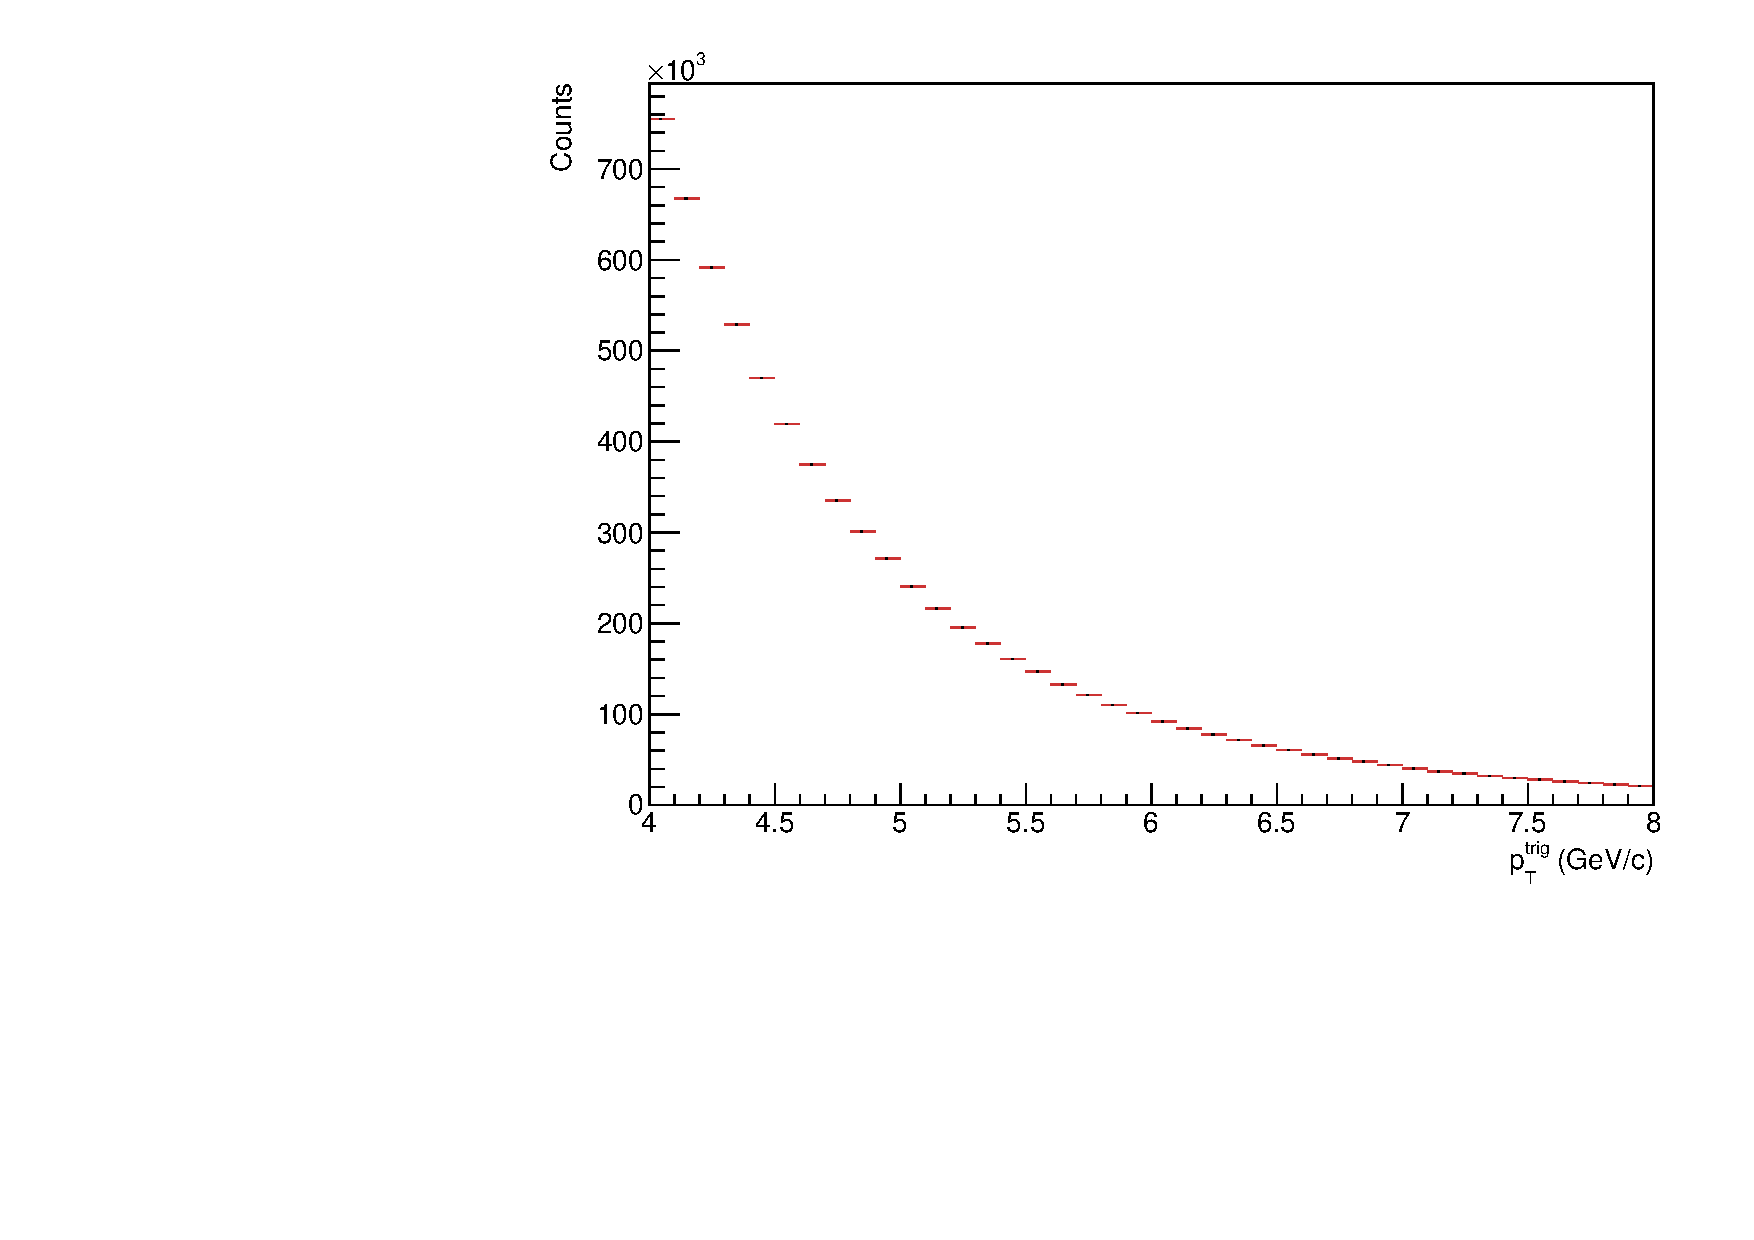
\includegraphics[width=\textwidth]{figures/analysis/trig_pt_dist_0_20.pdf}	
	\end{minipage}
	\begin{minipage}{0.32\textwidth}
		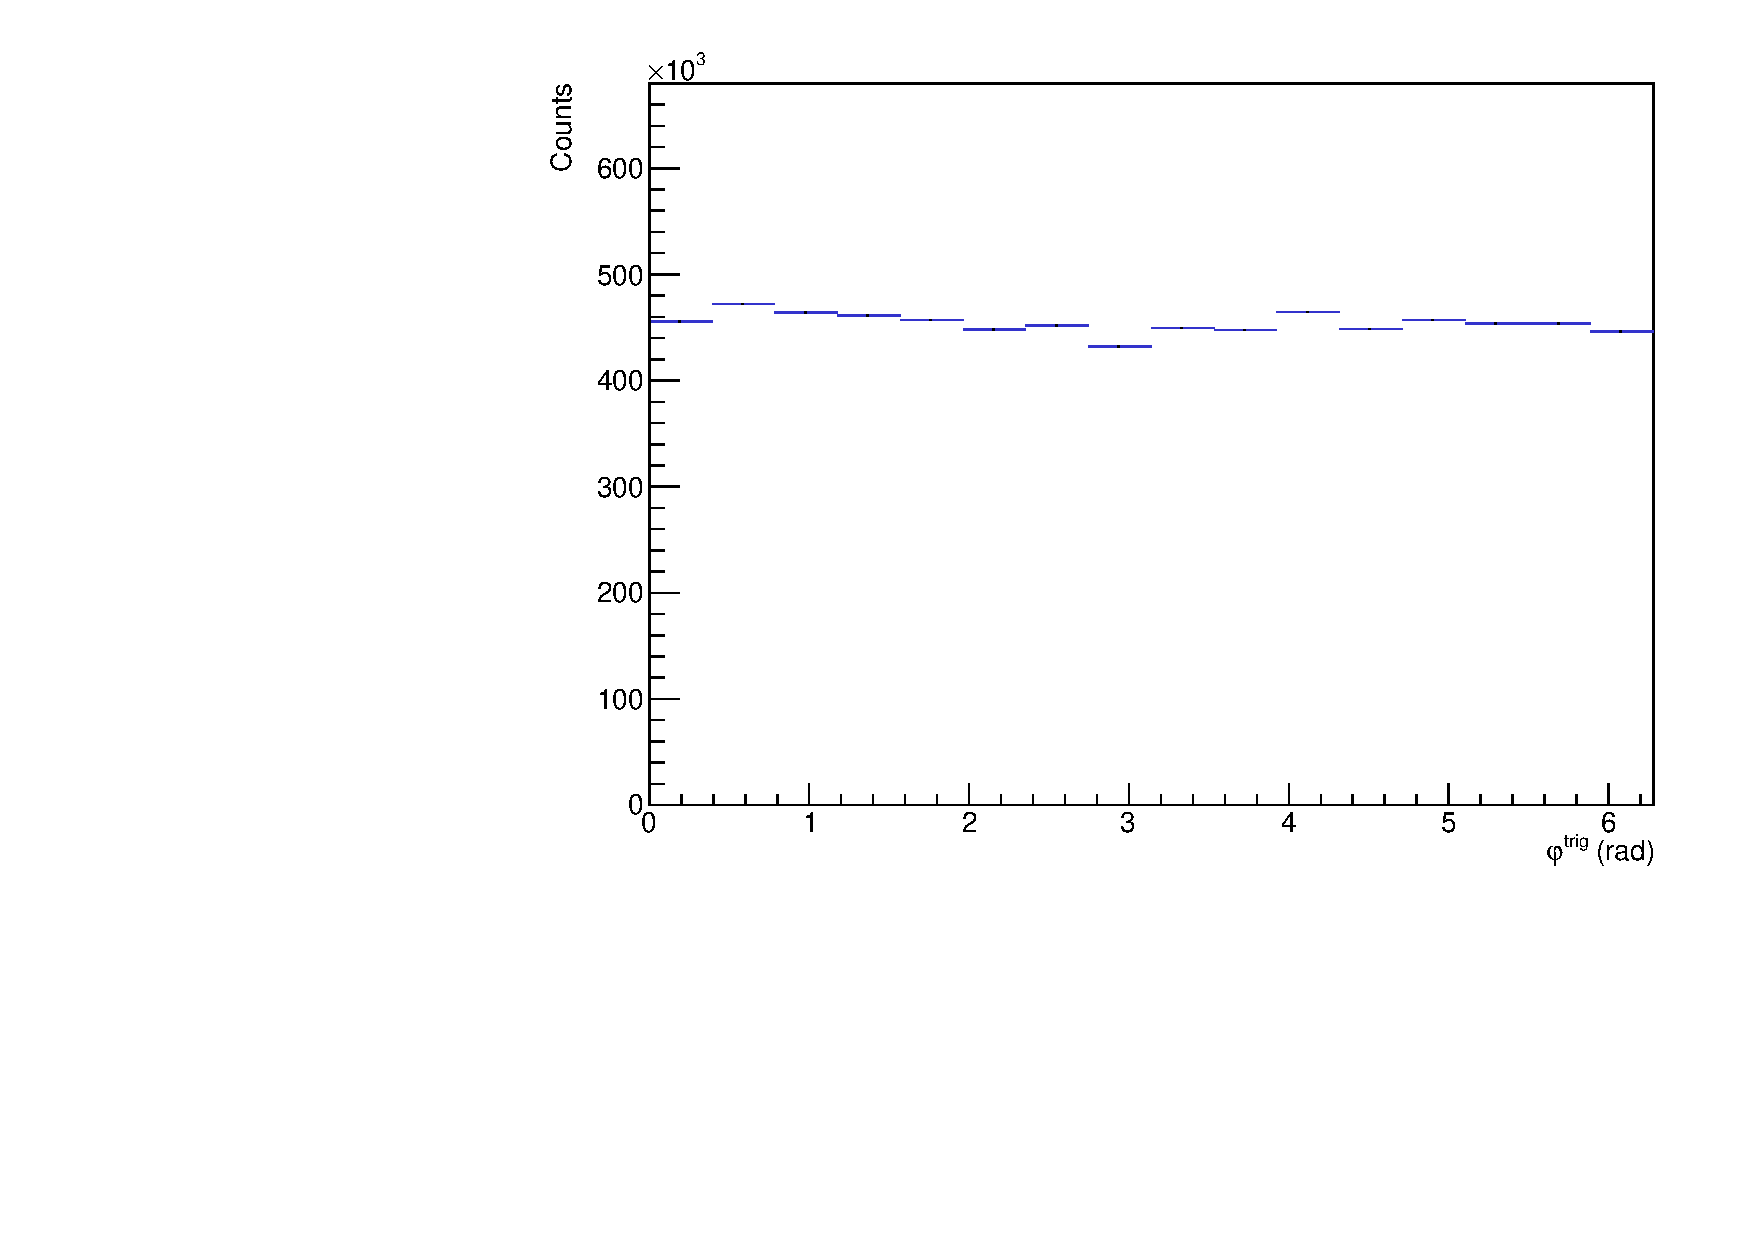
\includegraphics[width=\textwidth]{figures/analysis/trig_phi_dist_0_20.pdf}
	\end{minipage}
	\begin{minipage}{0.32\textwidth}
		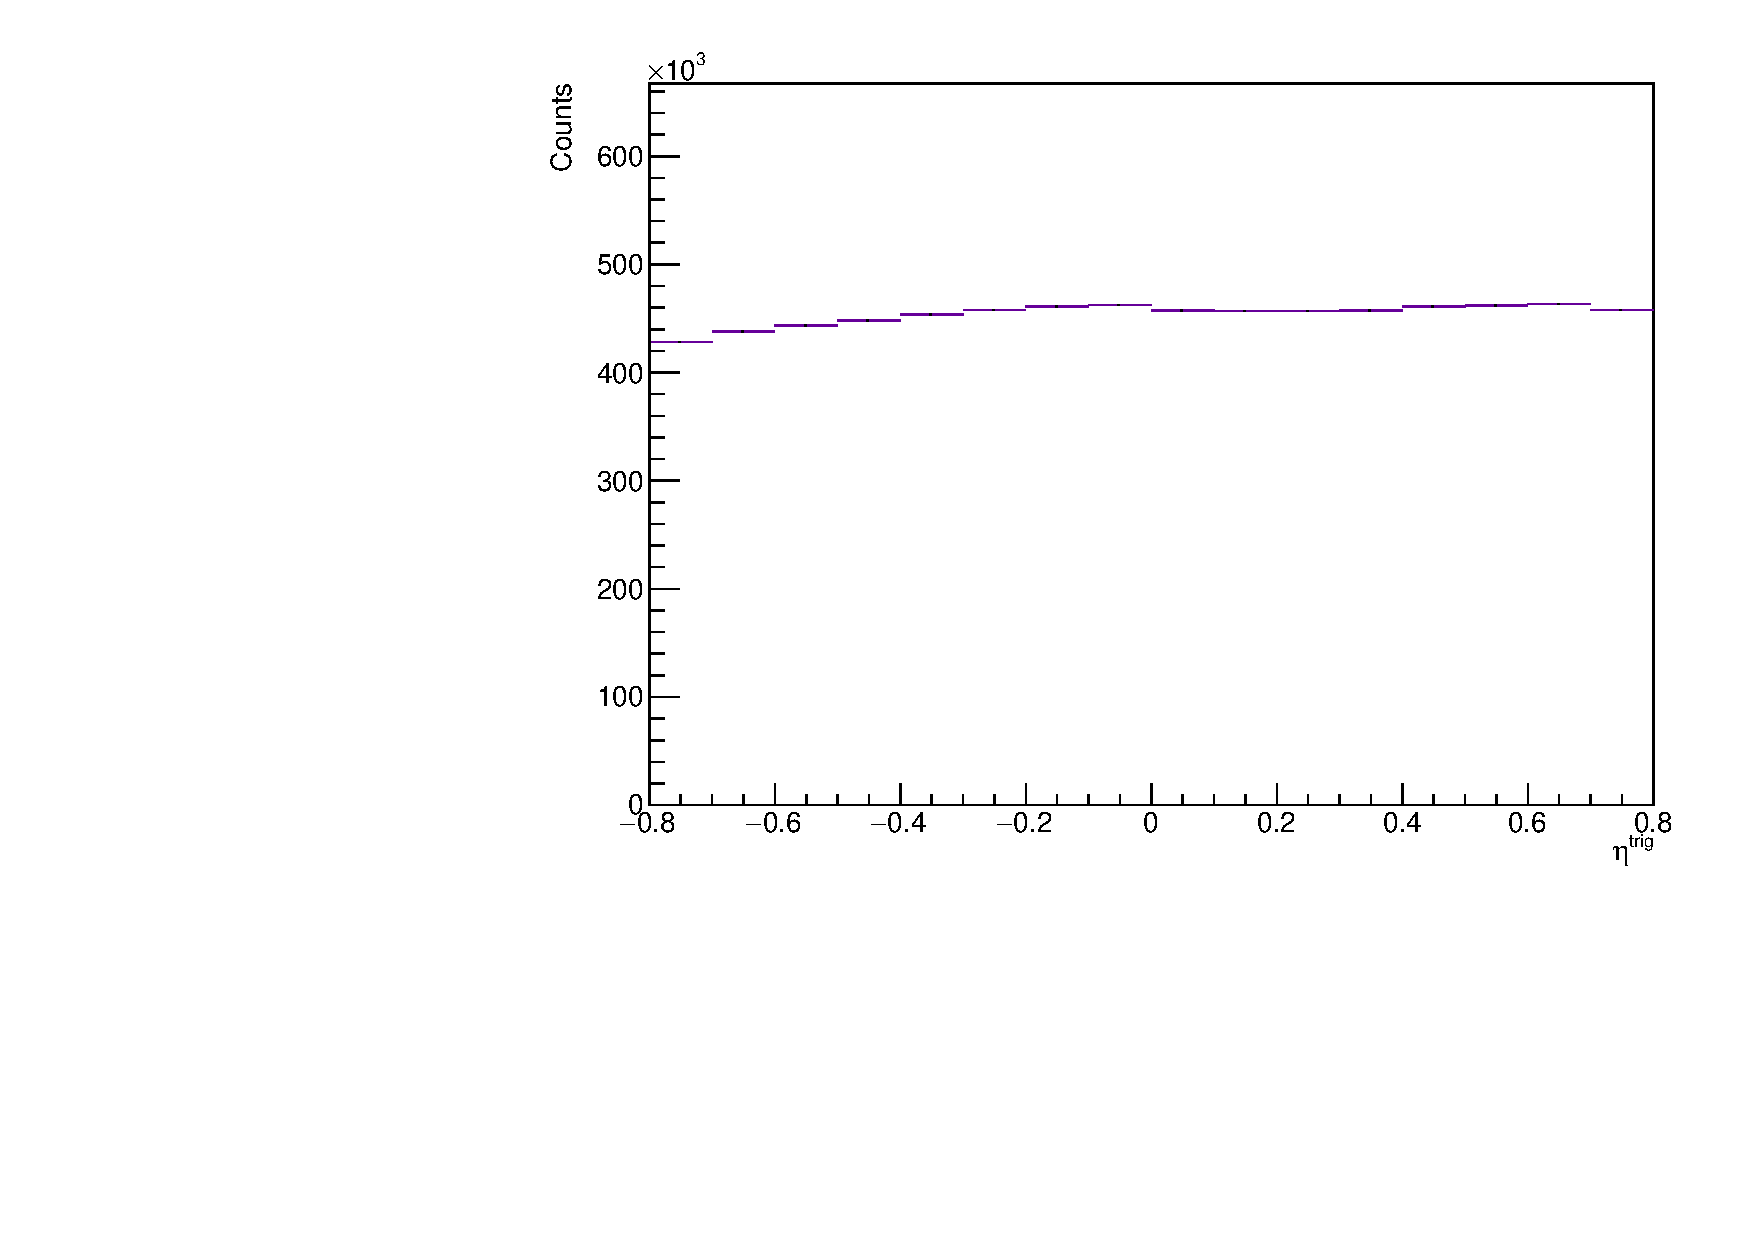
\includegraphics[width=\textwidth]{figures/analysis/trig_eta_dist_0_20.pdf}
	\end{minipage}
	\caption{The \pt (left), $\varphi$ (middle), and $\eta$ (right) distributions for the trigger hadrons in the multiplicity range 0-20\%.}
	\label{fig:trigger_plots}
\end{figure}

\begin{table}[h]
	\centering
	\caption{The track quality cuts applied to the trigger hadrons in this analysis.}
	\label{tab:trigger_track_cuts}
	\begin{tabular}{ l  c }
		\hline
		Selection criterion & Value \\
		\hline
		TPC clusters & $\geq 50$ \\
		$\chi^{2}$ per TPC cluster  & $<$ 4 \\
		Fraction of shared TPC clusters & $<$ 0.4 \\
		DCA$_{xy}$ & $< 2.4$ cm \\
		DCA$_{z}$ & $< 3.2$ cm \\
		Accept kink daughters & No \\
		\hline
	\end{tabular}
\end{table}

\subsection{Associated hadron track cuts}

To keep the results of this analysis more comparable to previous measurements of the $\Lambda/\pi \approx \Lambda/$h ratio, the selection criteria for the associated hadrons are more strict than those for the trigger hadrons as the associated hadrons are meant to be ``primary'', meaning they did not originate from a weak decay. All associated hadrons are required to meet the ALICE standard track quality cuts for primary charged hadrons described in Table~\ref{tab:primary_track_cuts}. Furthermore, the associated hadrons are selected only at midrapidity ($|\eta| < 0.8$) in the momentum region ${1.0 < p_{\text{T}} < 4.0 \text{GeV}/c}$. The \pt, $\varphi$ and $\eta$ distributions for the associated hadrons that pass these cuts in the 0-20\% multiplicity bin can be seen in Figure~\ref{fig:assoc_plots}.

\begin{figure}[t!]
	\centering
	\begin{minipage}{0.32\textwidth}
		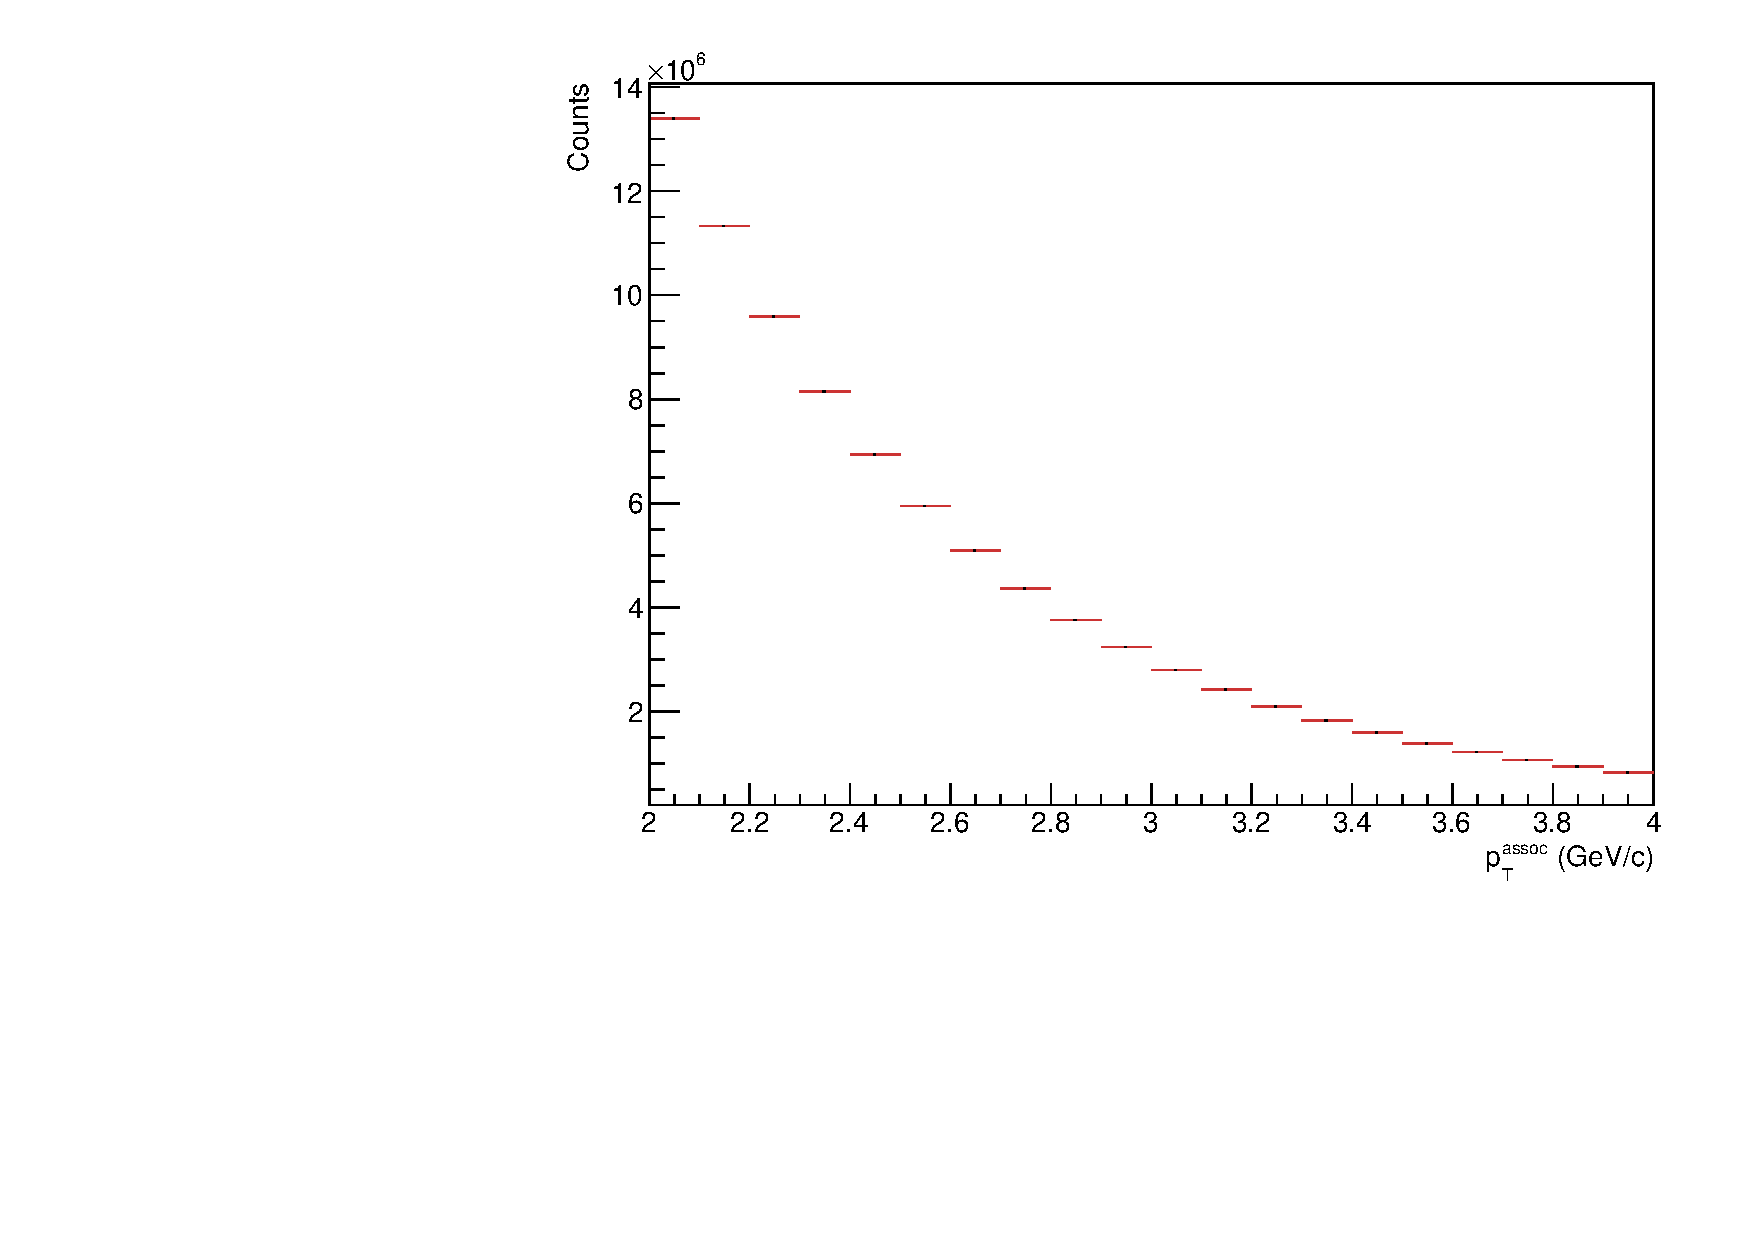
\includegraphics[width=\textwidth]{figures/analysis/assoc_pt_dist_0_20.pdf}
	\end{minipage}
	\begin{minipage}{0.32\textwidth}
		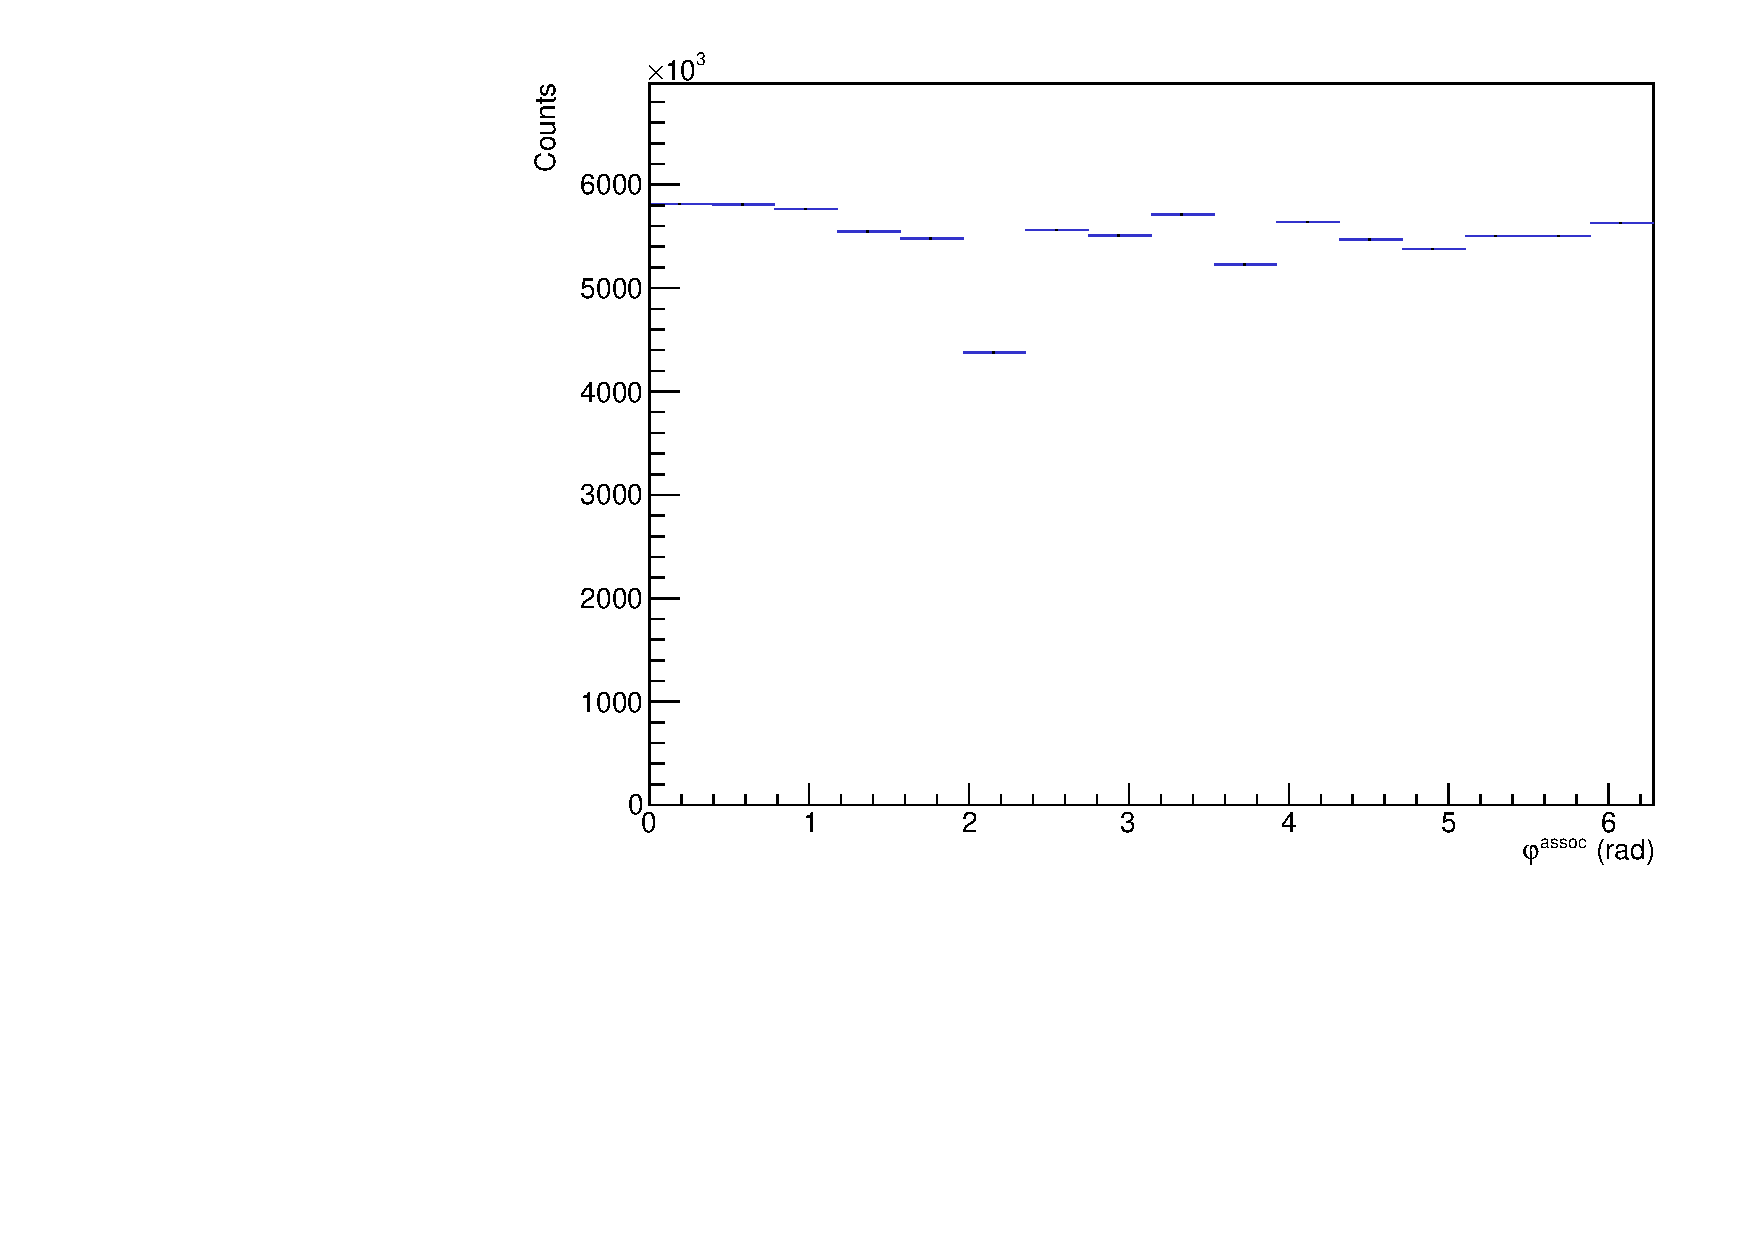
\includegraphics[width=\textwidth]{figures/analysis/assoc_phi_dist_0_20.pdf}
	\end{minipage}
	\begin{minipage}{0.32\textwidth}
		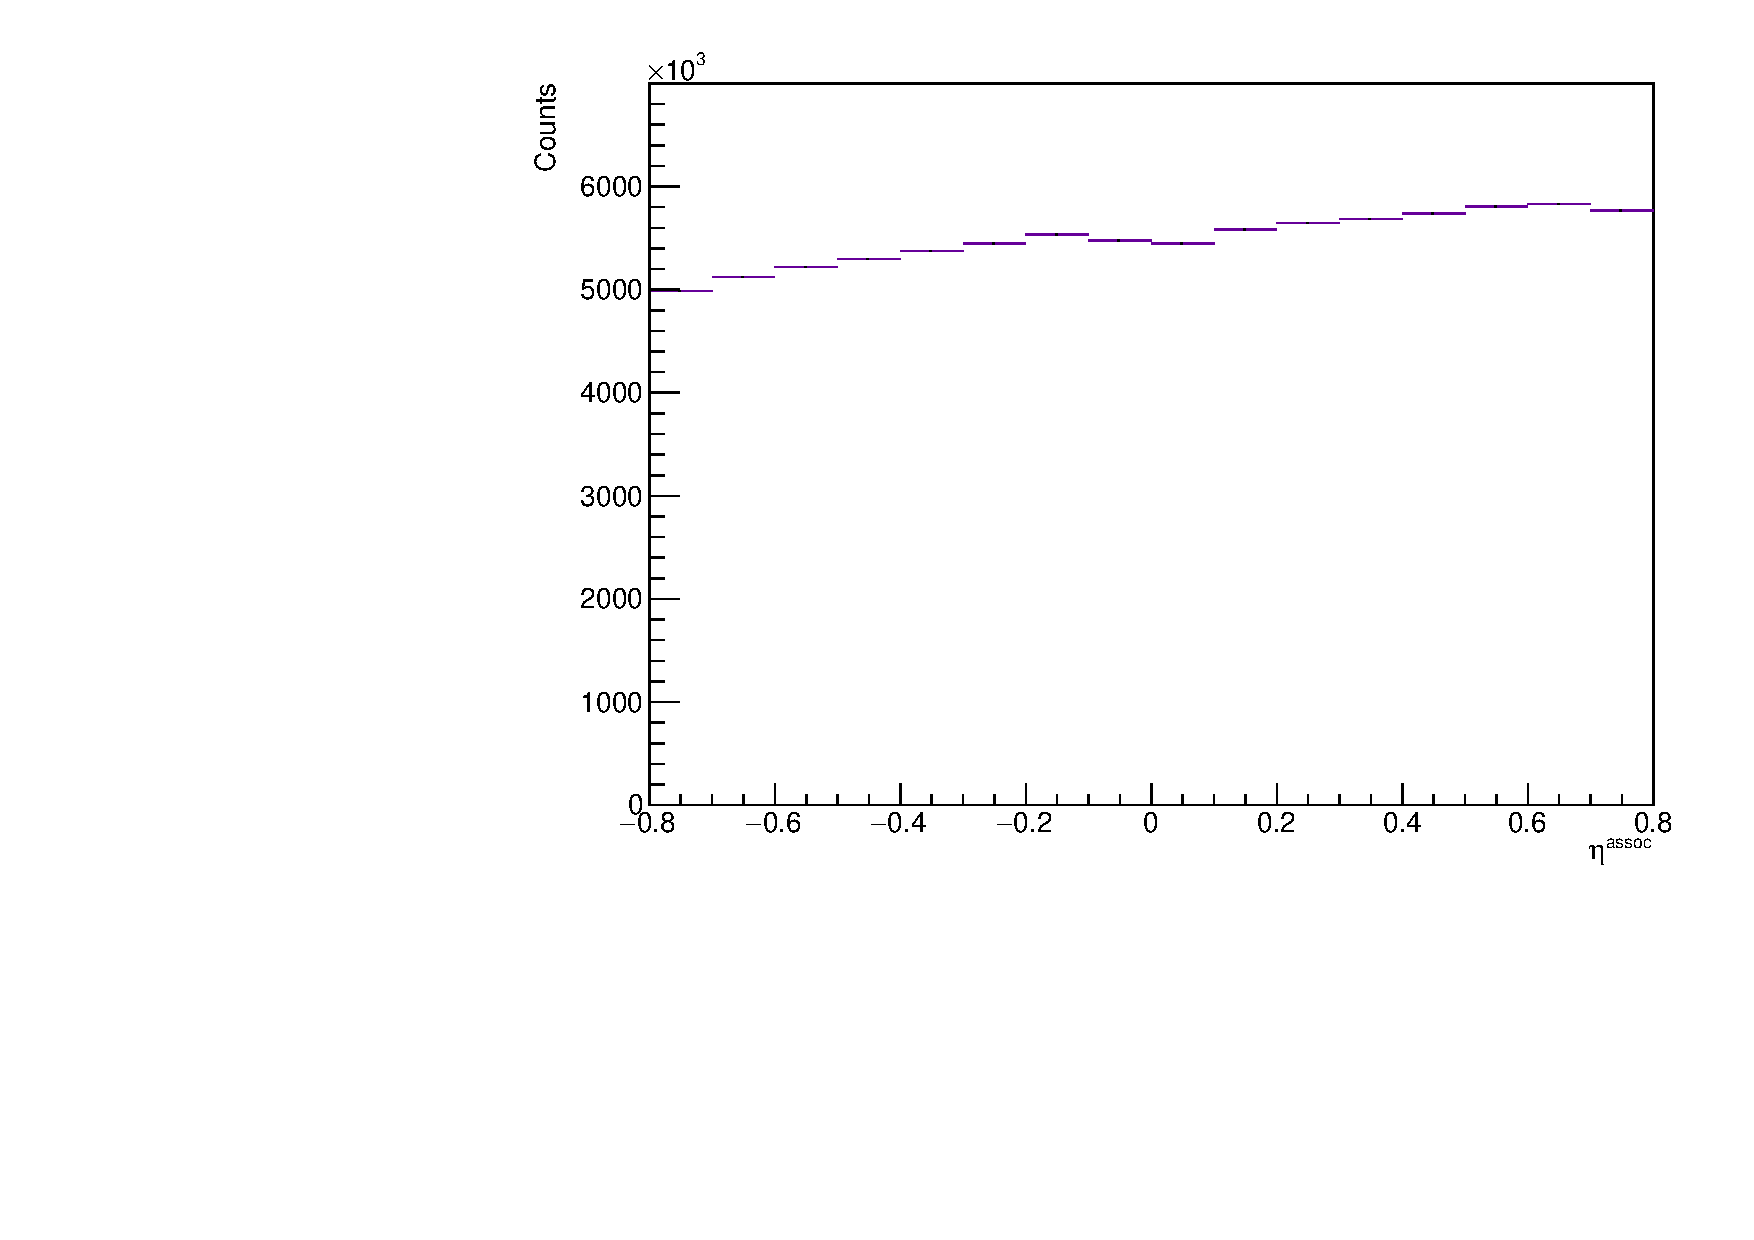
\includegraphics[width=\textwidth]{figures/analysis/assoc_eta_dist_0_20.pdf}
	\end{minipage}
	\caption{The \pt (left), $\varphi$ (middle), and $\eta$ (right) distributions for the associated hadrons in the multiplicity range 0-20\%. The dips observed in the $\varphi$ distribution are due to the TPC sector boundaries.}
	\label{fig:assoc_plots}
\end{figure}

\begin{table}[h]
	\centering
	\caption{The ALICE standard track quality cuts for primary charged hadrons, used for the selection of the associated hadrons in this analysis.}
	\label{tab:primary_track_cuts}
	\begin{tabular}{ l  c }
		\hline
		Selection criterion & Value \\
		\hline
		Crossed rows in TPC & $\geq$ 80 \\
		Crossed rows/findable clusters in TPC & $>$ 0.8 \\
		TPC clusters & $\geq 80$ \\
		ITS clusters & $\geq 3$ \\
		$\chi^{2}$ per TPC cluster  & $<$ 4 \\
		$\chi^{2}$ per ITS cluster  & $<$ 36 \\
		TPC and ITS refit required & Yes \\
		DCA$_{xy}$ & $< 0.0105 + 0.0350/p_{\text{T}}^{1.1}$ cm \\
		DCA$_{z}$ & $< 2$ cm \\
		\hline
	\end{tabular}
\end{table}

\section{$\Lambda$ reconstruction}
\label{sec:lambda_reconstruction}

\subsection{Characteristic V$^0$ decay topology}
\label{sec:v0_decay}

The $\Lambda$ candidates in this analysis are reconstructed using their characteristic ``V''-shaped decay topology, which is seen in the detector as two oppositely charged tracks originating from a common vertex which is sufficiently displaced from the PV (called the ``secondary vertex'' or SV). Such particles capable of being reconstructed via this topology are called ``V$^0$''s: the V describing the decay shape and the 0 indicating that the particle is neutral. A diagram depicting a typical V$^0$ decay is shown in Figure~\ref{fig:v0_decay}, with labels given for the most relevant kinematic variables.

\begin{figure}[h]
	\centering
	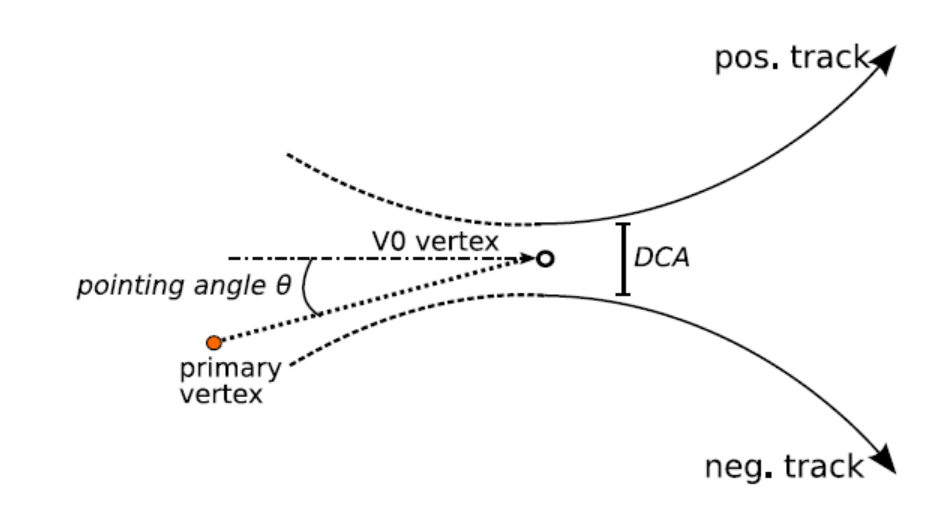
\includegraphics[width=0.5\textwidth]{figures/analysis/v0_decay.png}
	\caption{A diagram depicting a typical V$^0$ decay with labels for the most important kinematic variables. The diagram was taken from~\cite{V0Decay}.}
	\label{fig:v0_decay}
\end{figure}

The first and most important of these variables is the distance of closest approach (DCA) between the two tracks.\footnote{Note that the term DCA in this section refers to the distance of closest approach between the potential \lmb decay particles, whereas in Tables~\ref{tab:trigger_track_cuts} and~\ref{tab:primary_track_cuts}, DCA refers to the minimum distance between a given track and the PV.} This DCA needs to be small enough (relative to the tracking resolution) to ensure that the tracks originated from a common vertex. Another important variable is the transverse decay length of the V$^0$, which is the distance between the PV and the SV measured in the $xy$-plane. The importance of this variable is twofold: if the decay length is too small, then it may not even be possible to resolve the SV from the PV; and in addition, it allows for the distinction between V$^0$s of differing decay lengths. The final relevant variable is the cosine of the pointing angle, which is the angle between the momentum vector of the V$^0$ and the vector pointing from the PV to the SV. As V$^0$ candidates are generally required to be sufficiently collimated to ensure that the V$^0$ originated from the PV, the cosine of the pointing angle is usually close to unity.

Using these variables, a list of likely V$^0$ candidates is generated for each event, from which further cuts are applied to maximize the likelihood of the candidate being a true $\Lambda$ baryon. These cuts are summarized in the following section. There is also another technique for $\Lambda$ reconstruction whereby all oppositely charged proton-pion pairs are combined to form $\Lambda$ candidates, which is explored in more detail in Chapter~\ref{ch:systematics}. However, due to the large combinatorial background associated with this technique, the V$^0$ method described above is chosen as the \lmb reconstruction method for this analysis.


\subsection{$\Lambda$ daughter proton and pion track cuts}

Because of the longer decay length of the $\Lambda$ ($c\tau \approx 10$ cm), the corresponding daughter proton and pion tracks generally have fewer hits in both the ITS and TPC, resulting in ``lower quality'' track parameters. Because of this, the cuts applied to the daughter tracks used to reconstruct $\Lambda$ candidates are the least strict of all the track quality cuts in this analysis and are summarized in Table~\ref{tab:lambda_daughter_track_cuts}. The daughter proton and pion are also required to be at midrapidity ($|\eta| < 0.8$) and have a minimum $p_{\text{T}} >$ 0.15 GeV/$c$. 

\begin{table}[h]
	\centering
	\caption{The track quality cuts applied to both the daughter proton and pion tracks used to reconstruct $\Lambda$ candidates. These cuts are intentionally less strict than those applied to the trigger and associated hadrons as the daughter tracks are reconstructed from secondary particles.}
	\label{tab:lambda_daughter_track_cuts}
	\begin{tabular}{ l  c }
		\hline
		Selection criterion & Value \\
		\hline
		TPC refit required & Yes \\
		Crossed rows in TPC & $\geq$ 70 \\
		Crossed rows/findable clusters in TPC & $>$ 0.8 \\
		\hline
	\end{tabular}
\end{table}

Following the particle identification procedure outlined in Sections \ref{sec:tpc} and \ref{sec:tof}, the daughter proton and pion tracks are required to pass the following PID cuts using both the TPC and TOF detectors:

\begin{itemize}
	\item $|n\sigma_{\text{TPC}, p}| < 2$
	\item $|n\sigma_{\text{TPC}, \pi}| < 3$
	\item $|n\sigma_{\text{TOF}, p}| < 2$ (if signal exists)
	\item $|n\sigma_{\text{TOF}, \pi}| < 3$ (if signal exists)
\end{itemize}

The values of these cuts were chosen to maximize the $\Lambda$ signal while avoiding contamination from other particle species. The parenthetical ``if signal exists'' means that the TOF PID cut is only applied if the track has a TOF signal. Due to the large distance between the TOF detector and the PV, many lower momentum tracks are deflected by the magnetic field before reaching the TOF detector, resulting in no signal. Excluding such tracks results in a more pure sample of protons and pions, at the cost of a much lower number of $\Lambda$ candidates. While such a cost is not acceptable for this analysis, the effect of excluding these tracks is investigated in Chapter~\ref{ch:systematics}. The $n\sigma$ distributions for both the TPC and TOF detectors of the daughter proton and pion tracks that pass the aforementioned quality cuts are shown in Figure~\ref{fig:nsigma_tpc} and Figure~\ref{fig:nsigma_tof}, respectively. To check for contamination from other particle species, the TOF and TPC information is combined to form a $n\sigma_{\text{TOF}}$ vs $n\sigma_{\text{TPC}}$ plot, which is shown for both the protons and pions in Figure~\ref{fig:nsigma_tof_v_tpc}. No contamination is observed for either the proton or pion tracks.

\begin{figure}[h]
	\centering
	\begin{minipage}{0.48\textwidth}
		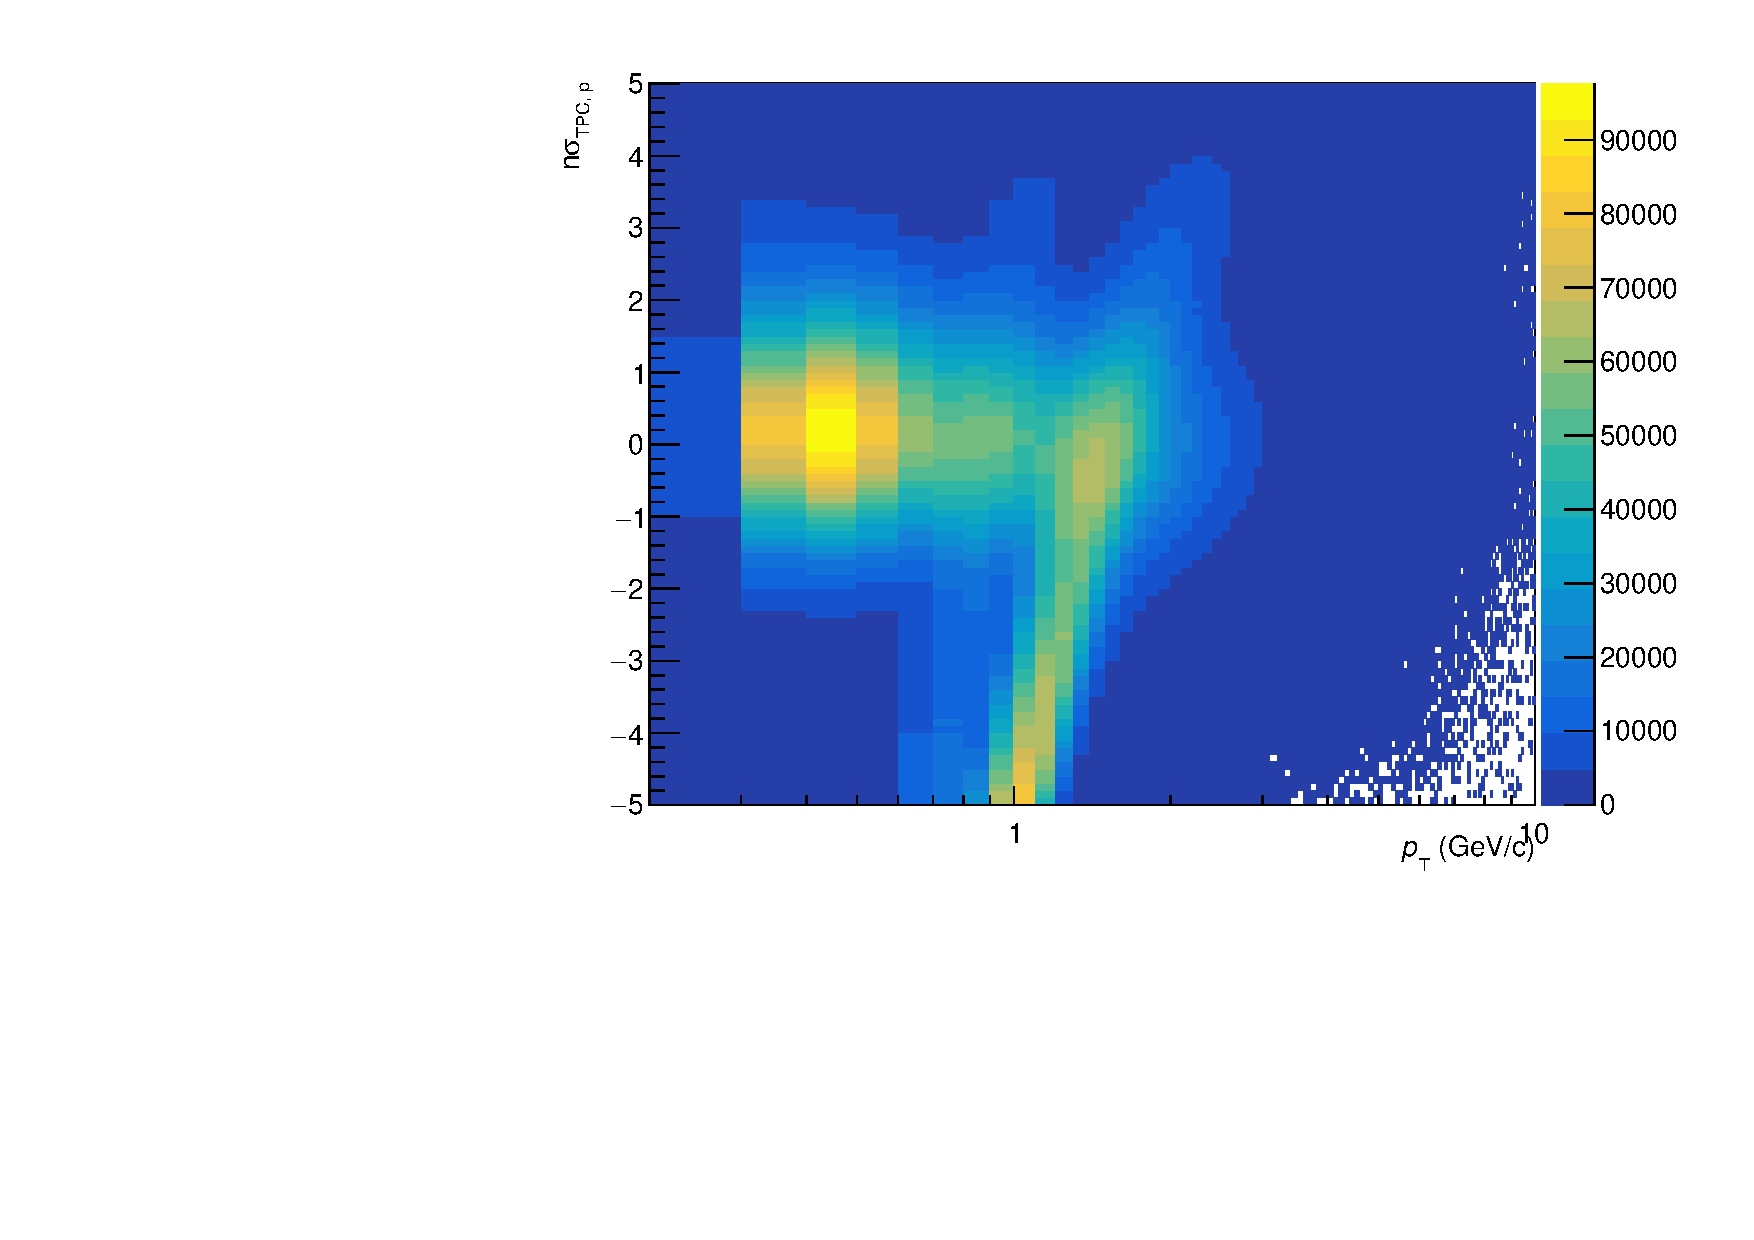
\includegraphics[width=\textwidth]{figures/analysis/nsigma_tpc_proton.pdf}
	\end{minipage}
	\begin{minipage}{0.48\textwidth}
		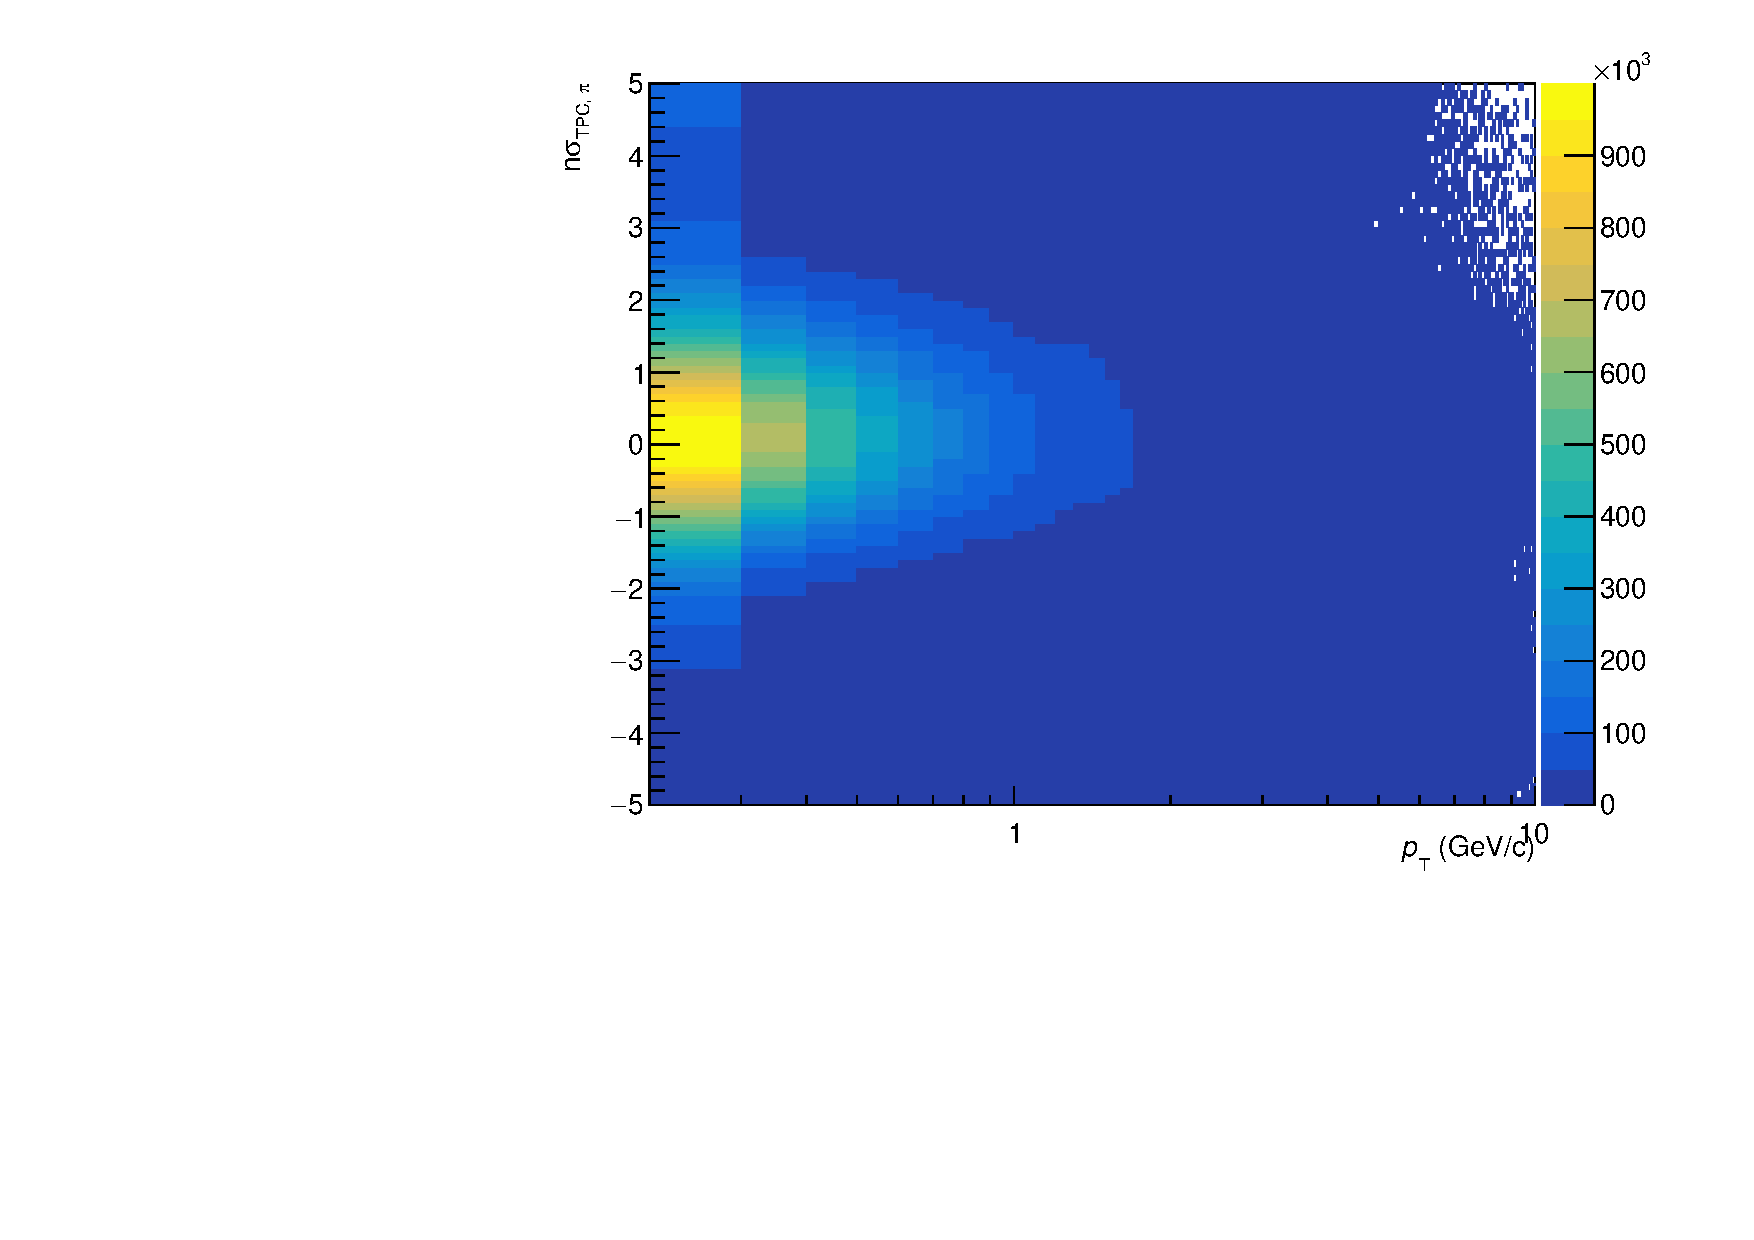
\includegraphics[width=\textwidth]{figures/analysis/nsigma_tpc_pion.pdf}
	\end{minipage}
    \caption{$n\sigma$ for protons (left) and pions (right) in the TPC detector as a function of $p_{T}$.}
	\label{fig:nsigma_tpc}
\end{figure}

\begin{figure}[h]
	\centering
	\begin{minipage}{0.48\textwidth}
		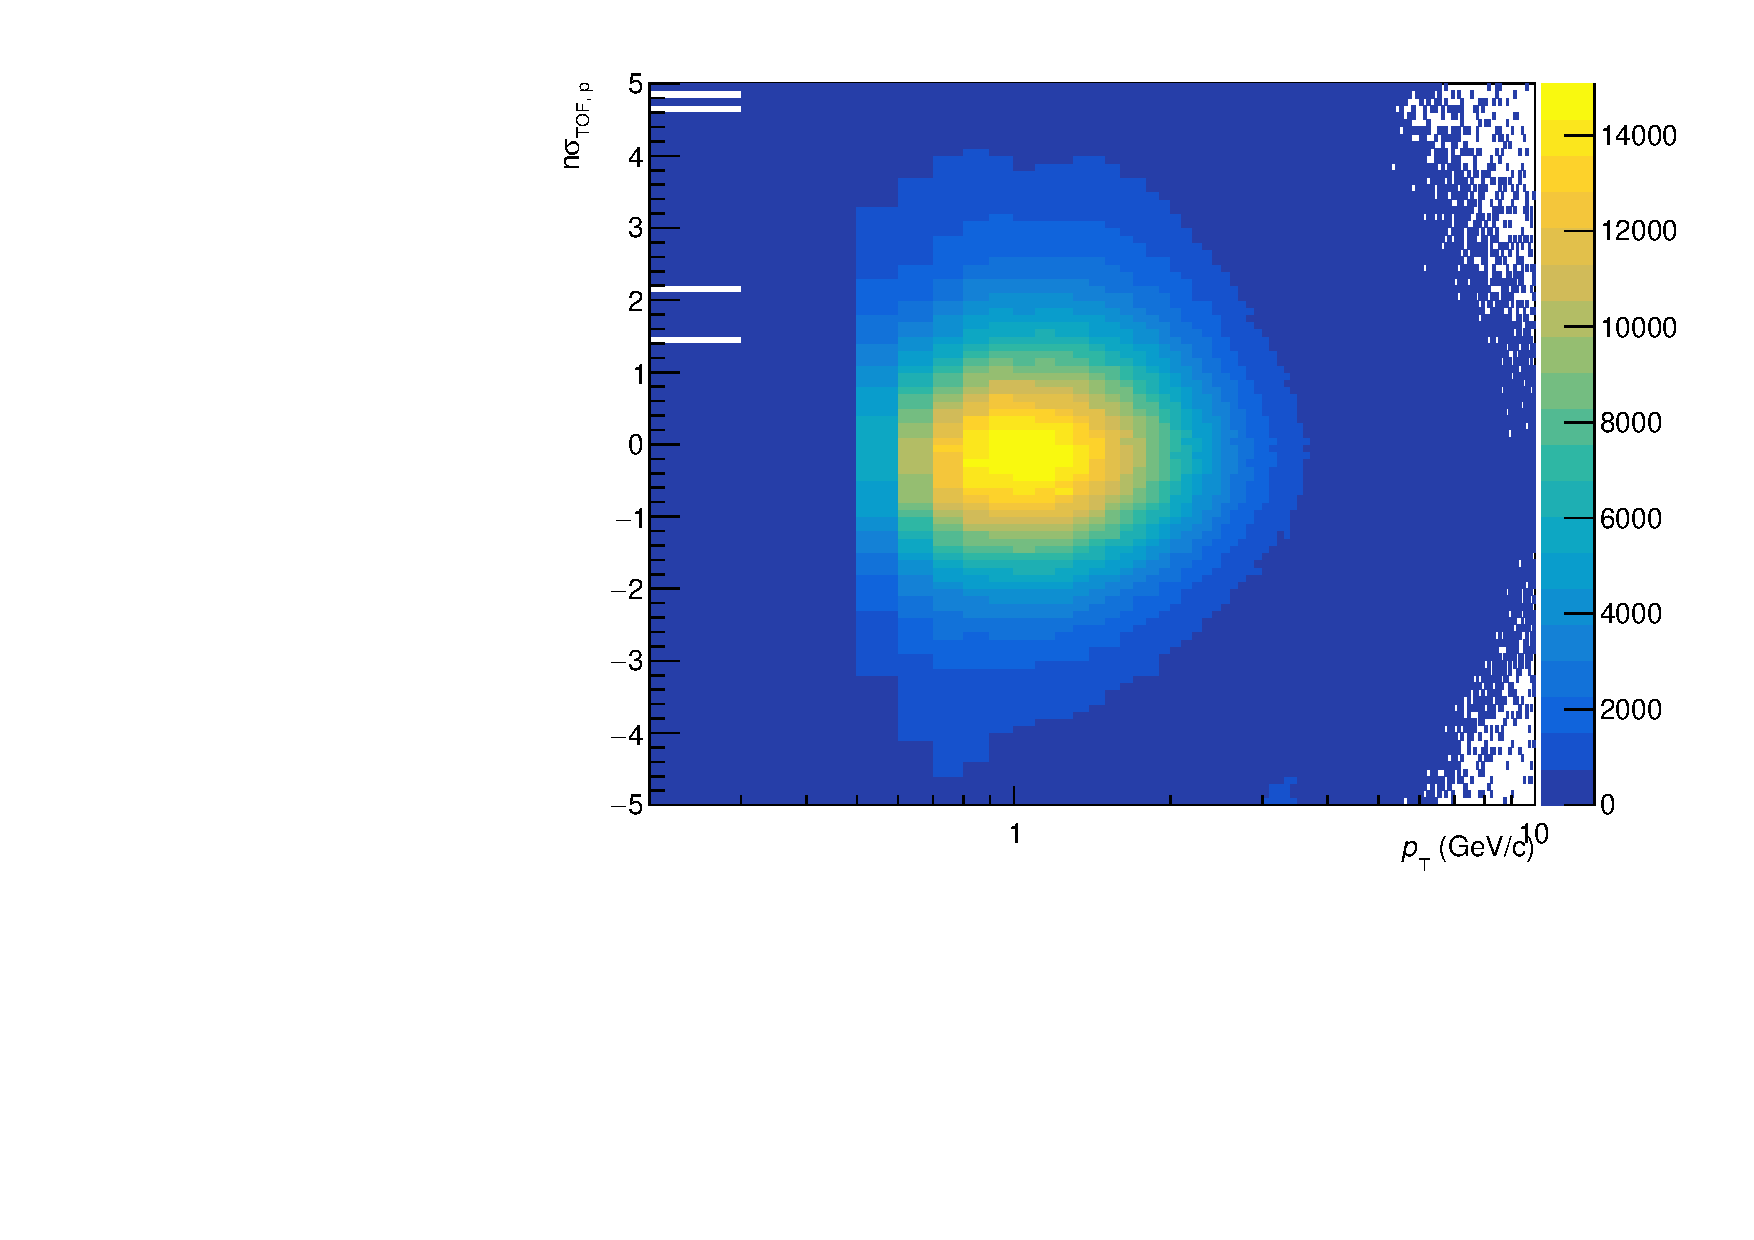
\includegraphics[width=\textwidth]{figures/analysis/nsigma_tof_proton.pdf}
	\end{minipage}
	\begin{minipage}{0.48\textwidth}
		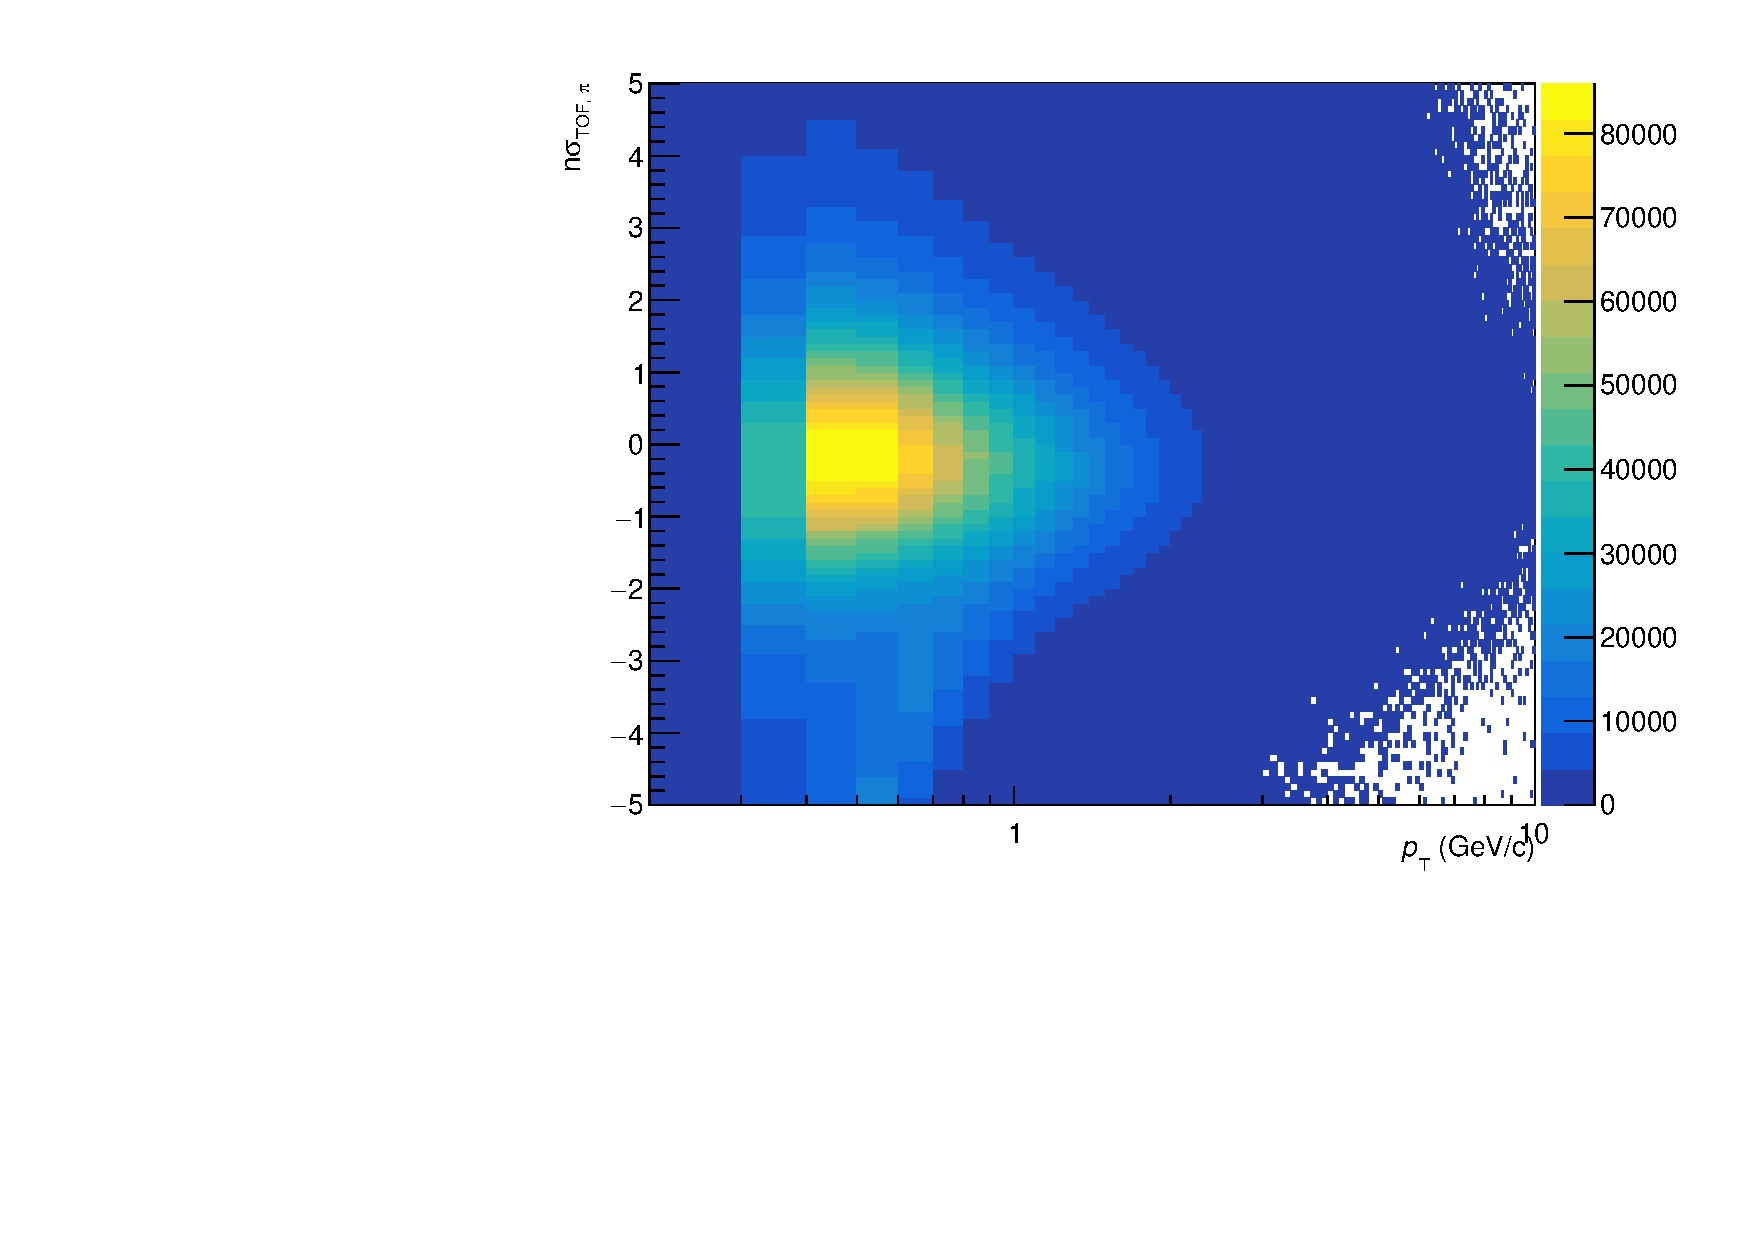
\includegraphics[width=\textwidth]{figures/analysis/nsigma_tof_pion.pdf}
	\end{minipage}
    \caption{$n\sigma$ for protons (left) and pions (right) in the TOF detector as a function of $p_{T}$.}
	\label{fig:nsigma_tof}
\end{figure}

\clearpage

\begin{figure}[h]
	\centering
	\begin{minipage}{0.48\textwidth}
		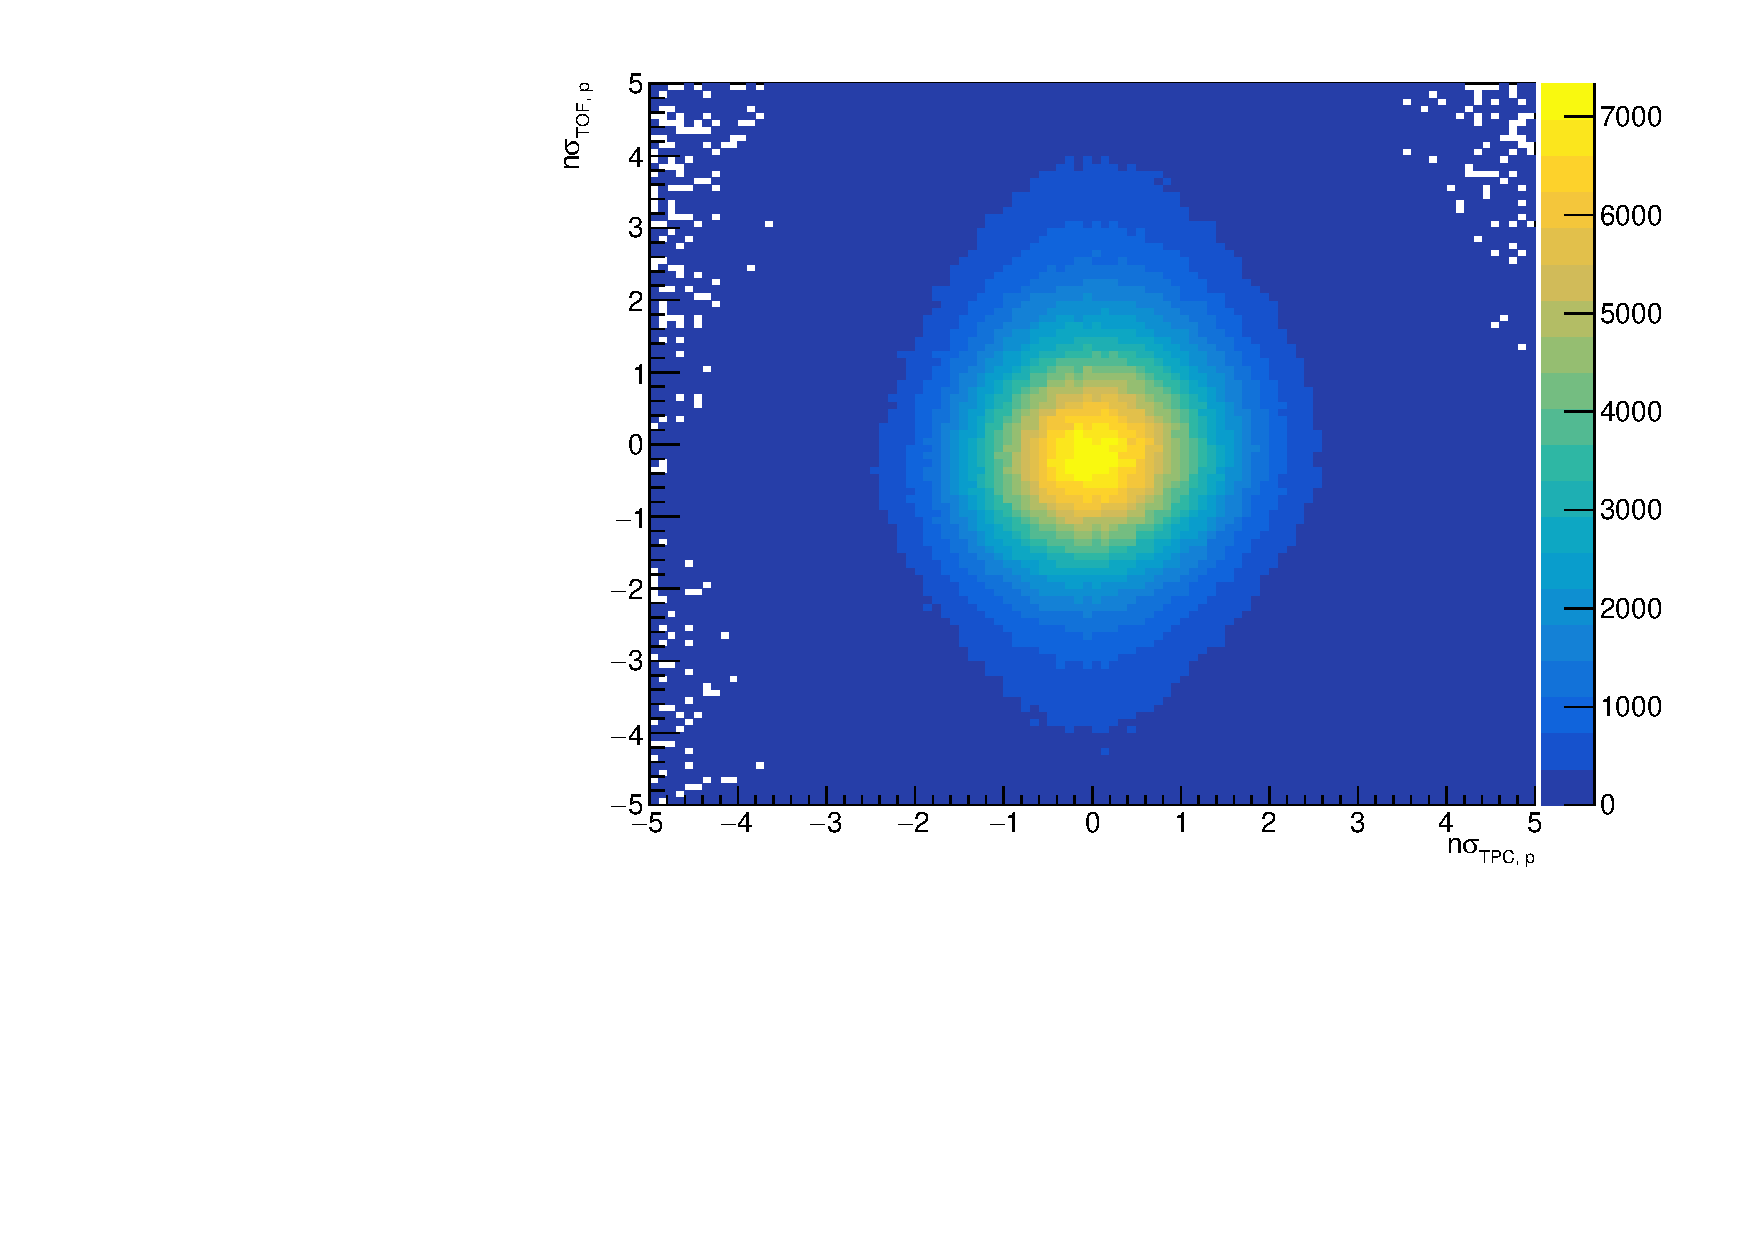
\includegraphics[width=\textwidth]{figures/analysis/nsigma_tof_v_tpc_proton.pdf}
	\end{minipage}
	\begin{minipage}{0.48\textwidth}
		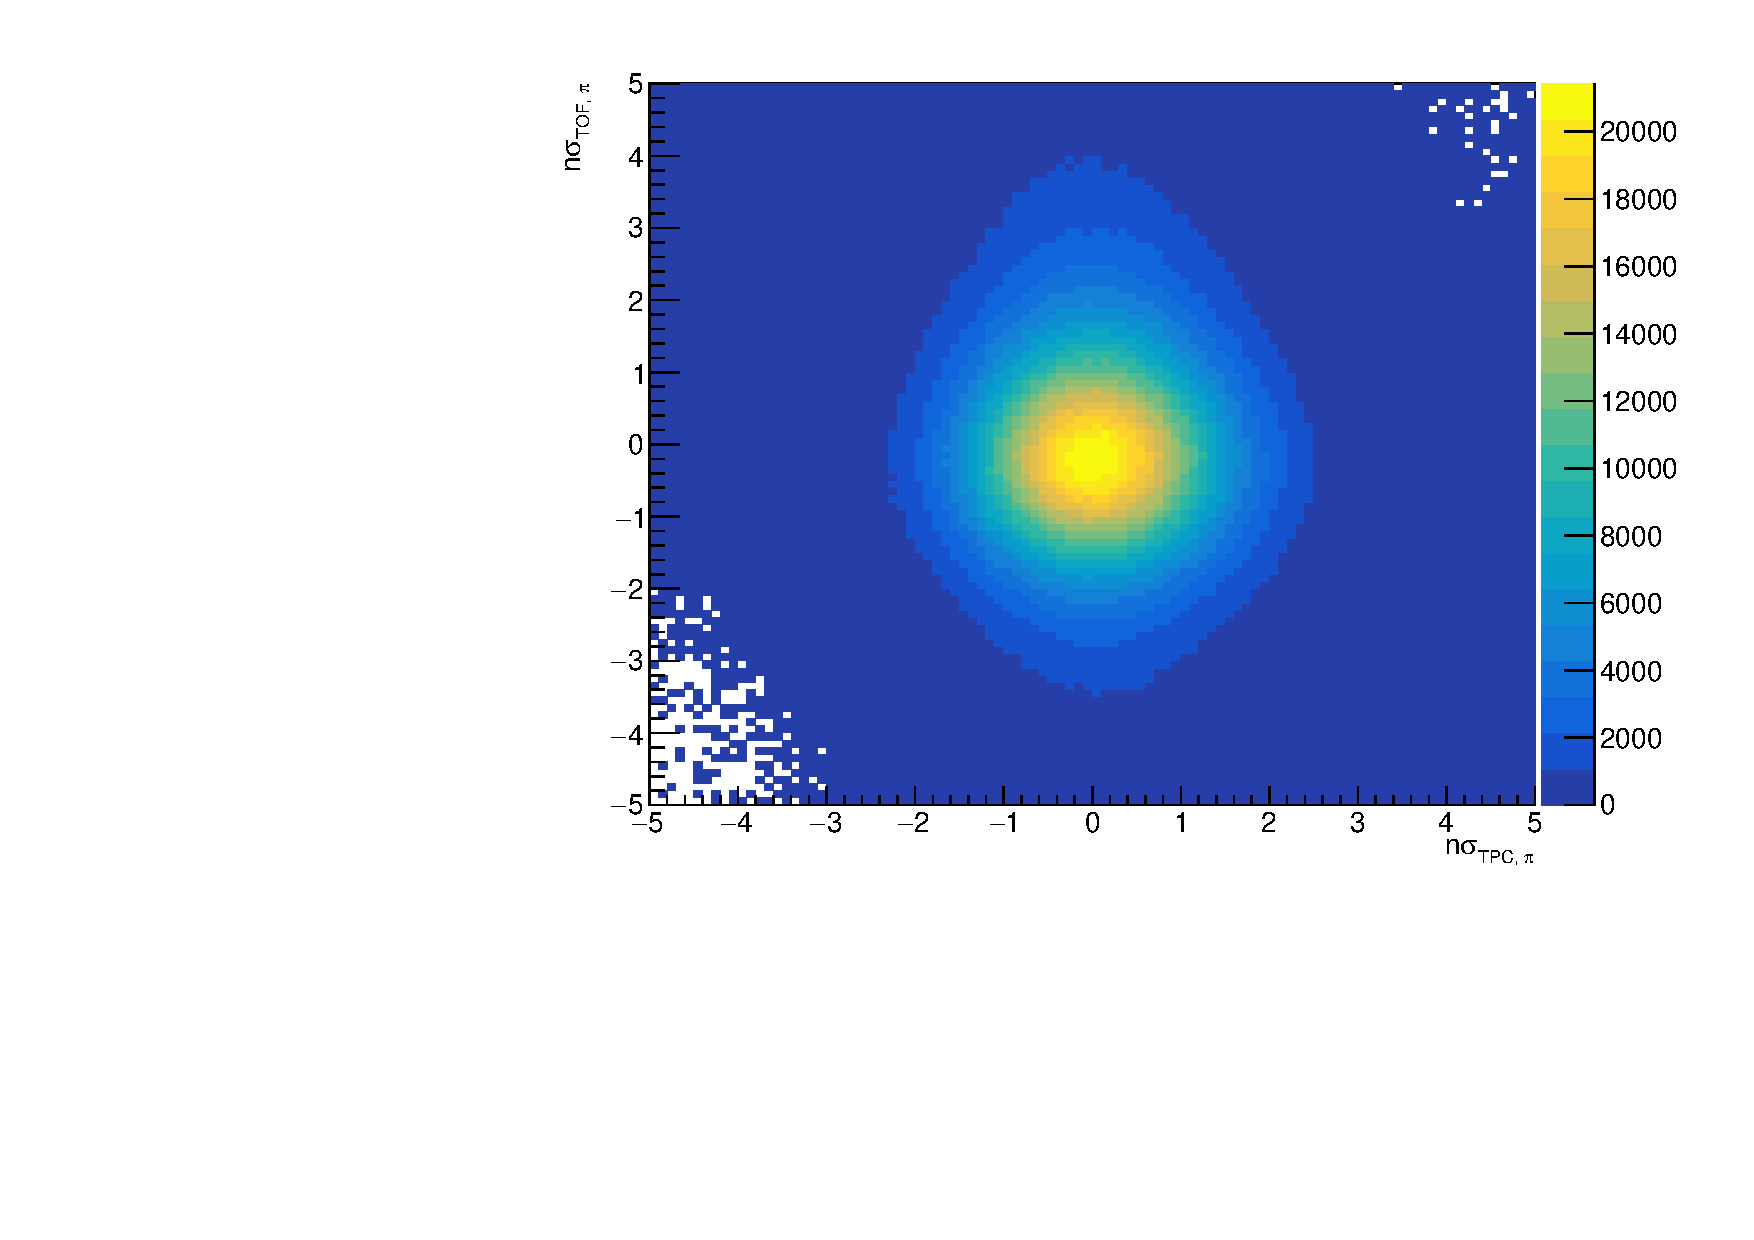
\includegraphics[width=\textwidth]{figures/analysis/nsigma_tof_v_tpc_pion.pdf}
	\end{minipage}
    \caption{$n\sigma$ in TOF vs $n\sigma$ in TPC for protons (left) and pions (right). No contimatination is observed for both of the particle species.}
	\label{fig:nsigma_tof_v_tpc}
\end{figure}

\subsection{$\Lambda$ candidate selection}

With the daughter proton and pion tracks selected, the $\Lambda$ candidates are generated by combining all oppositely charged proton-pion pairs into V$^0$s which meet the topological selection criteria described in Table~\ref{tab:lambda_selection}. 

\begin{table}[h!]
	\centering
	\caption{Topological selection criteria applied to $\Lambda$ candidates.}
	\label{tab:lambda_selection}
	\begin{tabular}{l c}
		\hline
		Selection criterion & Value \\
		\hline
		$|\eta|$ & $< 0.8$ \\
		Decay radius (cm) & $> 0.2$ \\
		DCA$_{xy}$ of pion track to PV (cm) & $> 0.06$ \\
		DCA$_{xy}$ of proton track to PV (cm) & $> 0.06$ \\
		DCA$_{xy}$ between daughter tracks (n$\sigma$) & $< 1.5$ \\
		cos($\theta_{\text{pointing}}$) & $> 0.9$ \\
		Invariant mass (\GeV/$c^2$) & $1.102 < M_{p\pi} < 1.130$ \\
		\hline
	\end{tabular}
\end{table}

\noindent The invariant mass $M_{p\pi}$ is calculated using
%
\begin{equation}
	M_{p\pi} = \sqrt{(E_{p} + E_{\pi})^2 - (\vec{p}_{p} + \vec{p}_{\pi})^2},
\end{equation}
%
where $E_{x} = \sqrt{m_{x}^2 + p_{x}^2}$ is the energy of the particle of species $x$. The $M_{p\pi}$ distributions for the $\Lambda$ candidates for all multiplicity and momentum bins are shown in Figure~\ref{fig:lambda_mass}. The distributions are also fit with a Voigtian function (convolution of Breit-Wigner and Gaussian~\cite{Voigt}) plus a straight line to describe the background. Note that despite the selection criteria, there is still a non-negligible background due to the presence of misidentified $\Lambda$ candidates. As this background inevitably makes its way into the final h-$\Lambda$ correlation distributions, it is removed using the technique described in Section~\ref{sec:comb_bg_removal}. 


\begin{figure}[ht]
	\centering
	\begin{minipage}{0.48\textwidth}
		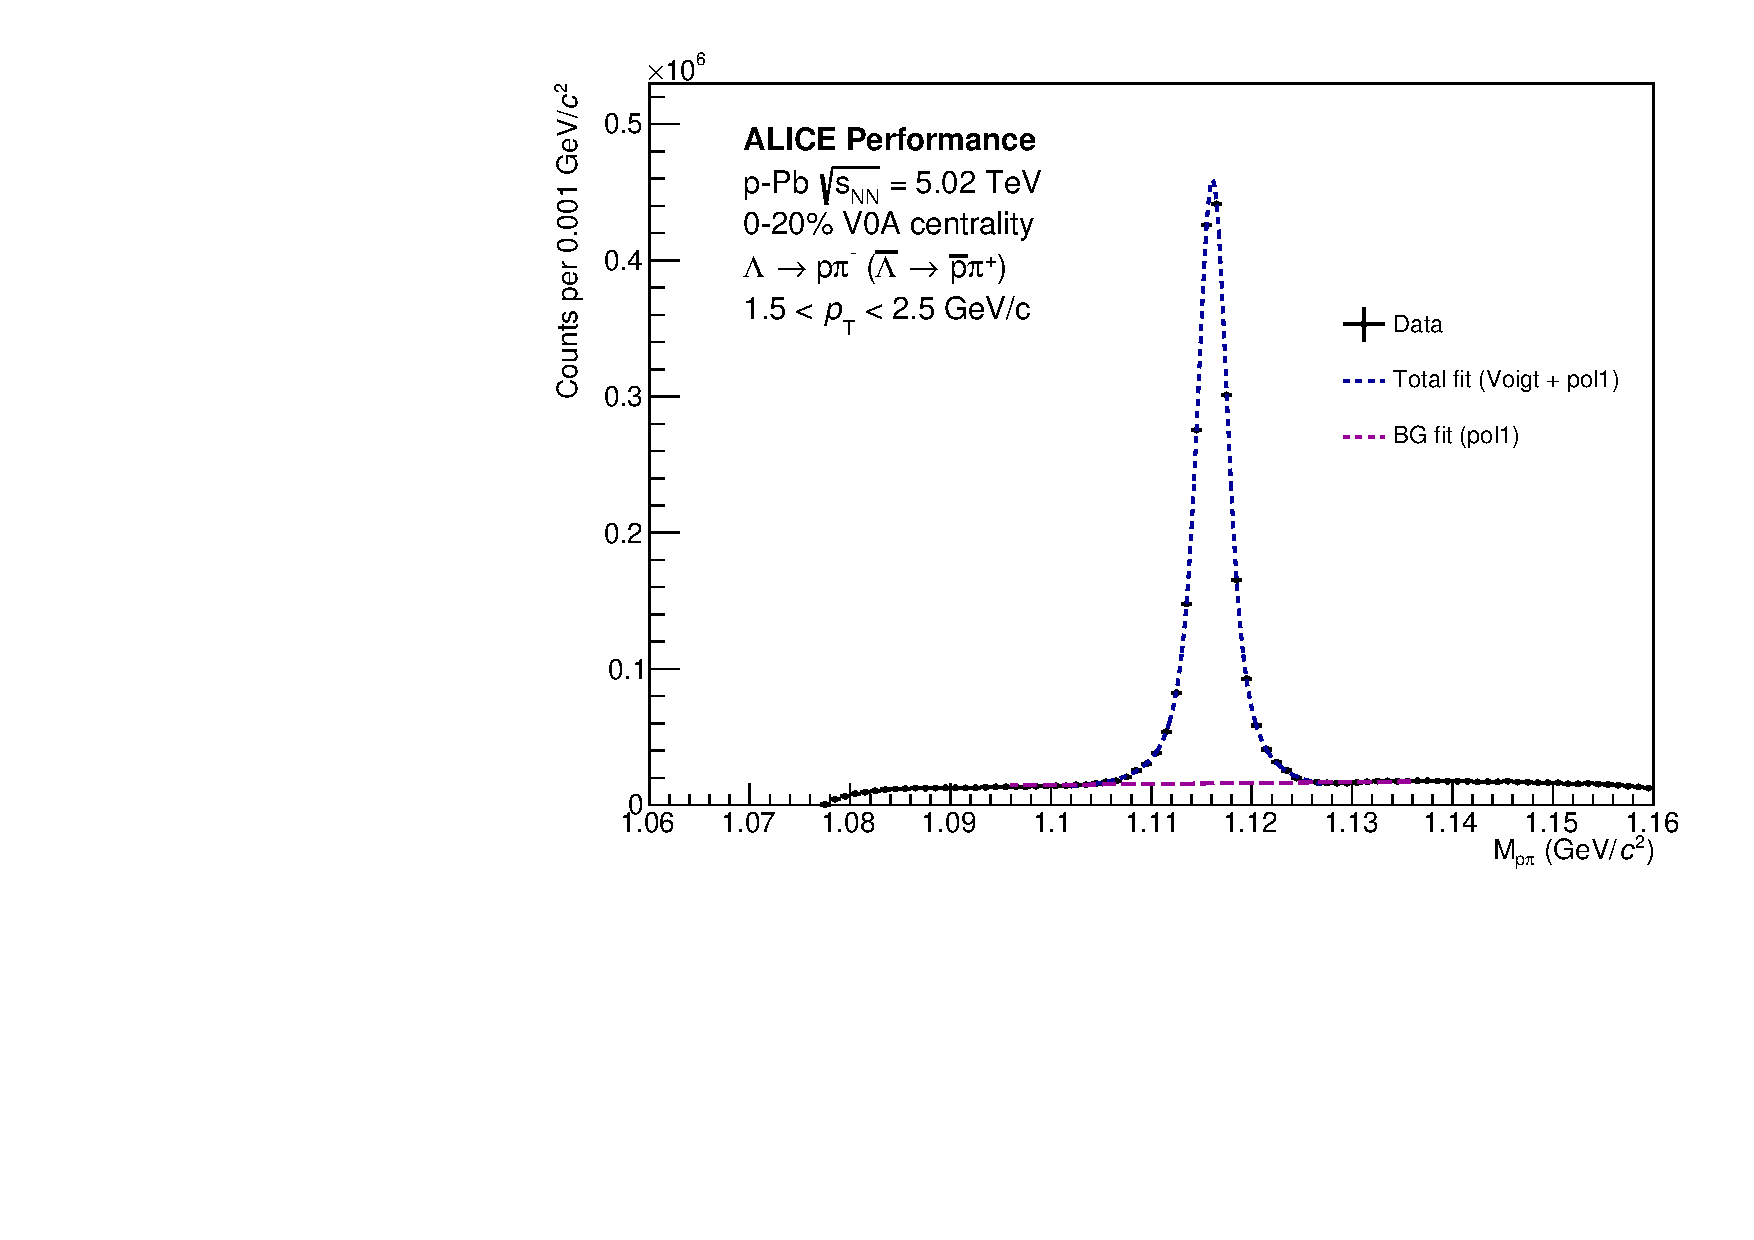
\includegraphics[width=\textwidth]{figures/analysis/lambda_mass_dist_0_20_lowpt.pdf}
	\end{minipage}
	\begin{minipage}{0.48\textwidth}
		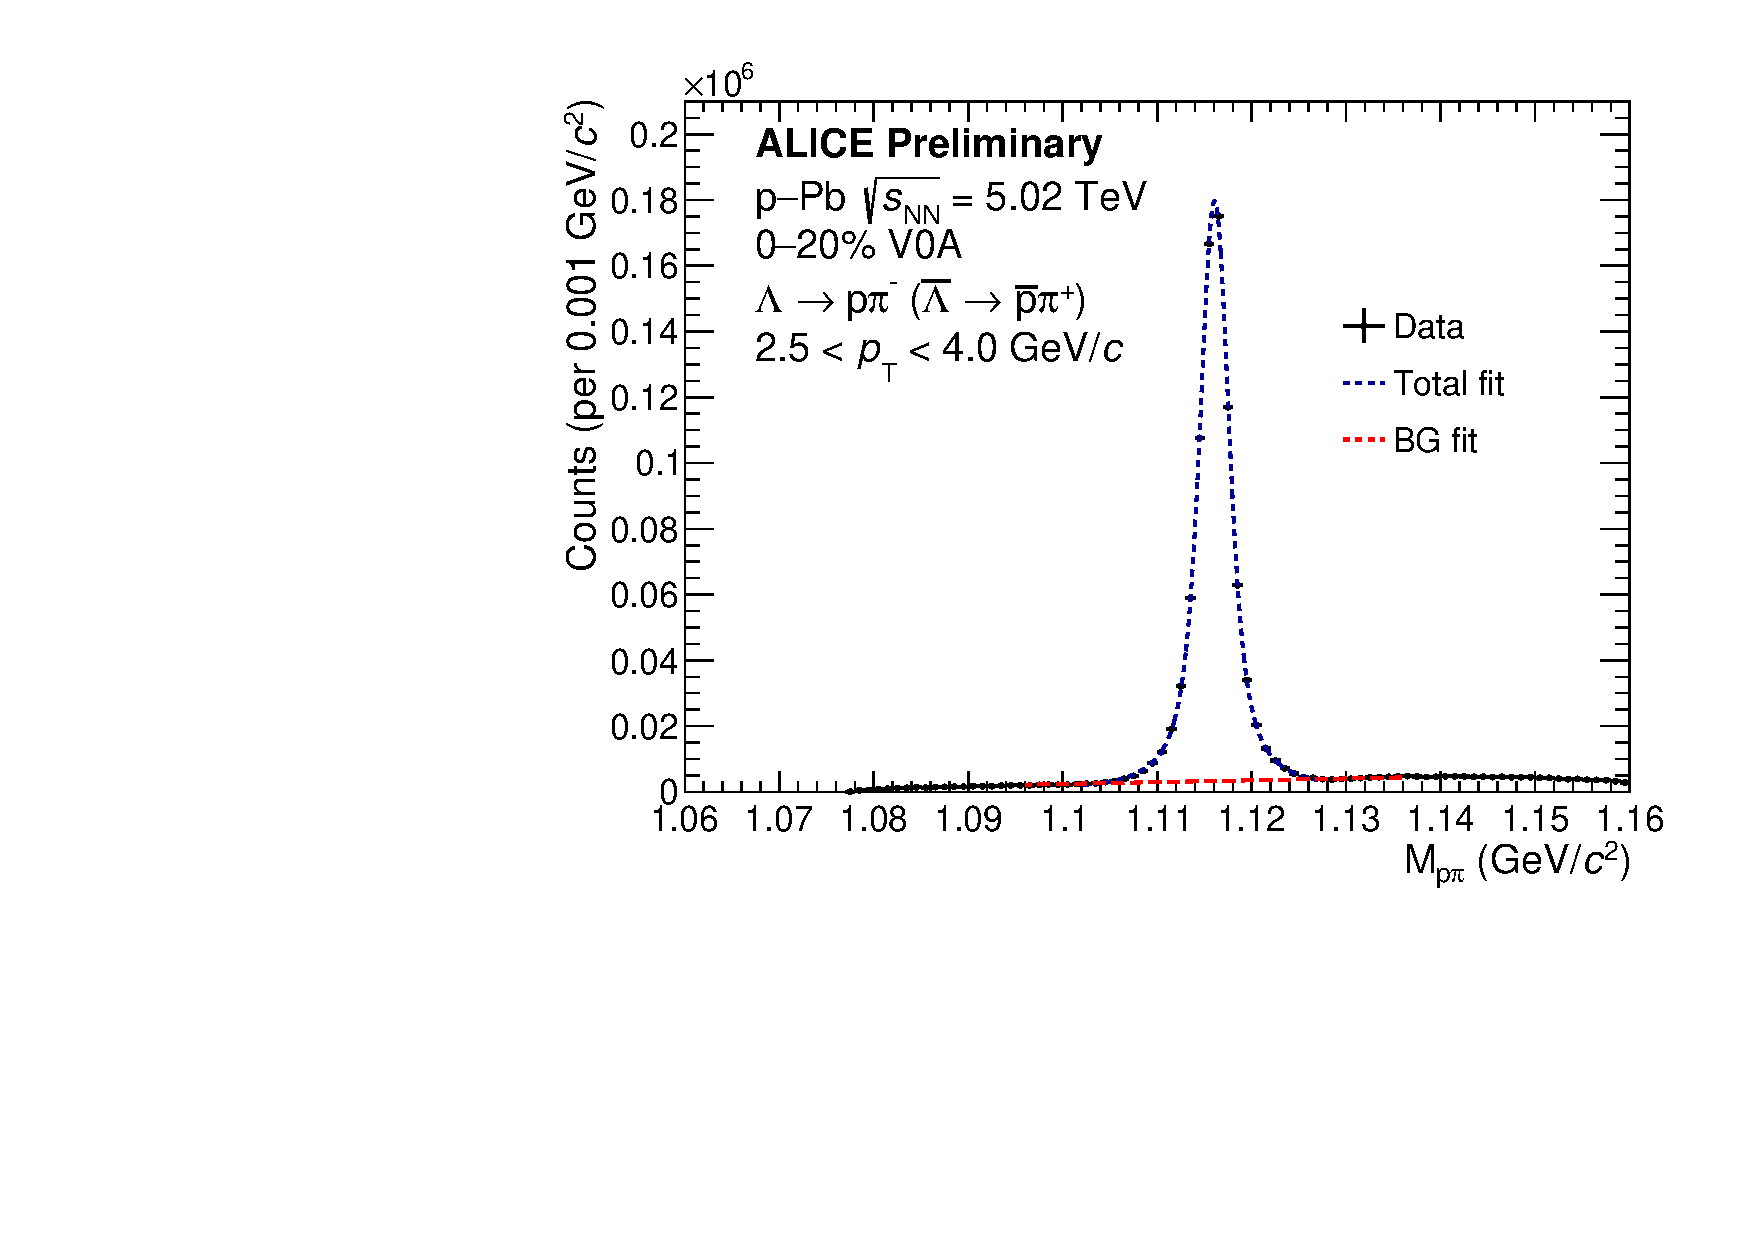
\includegraphics[width=\textwidth]{figures/analysis/lambda_mass_dist_0_20_highpt.pdf}
	\end{minipage}
	\begin{minipage}{0.48\textwidth}
		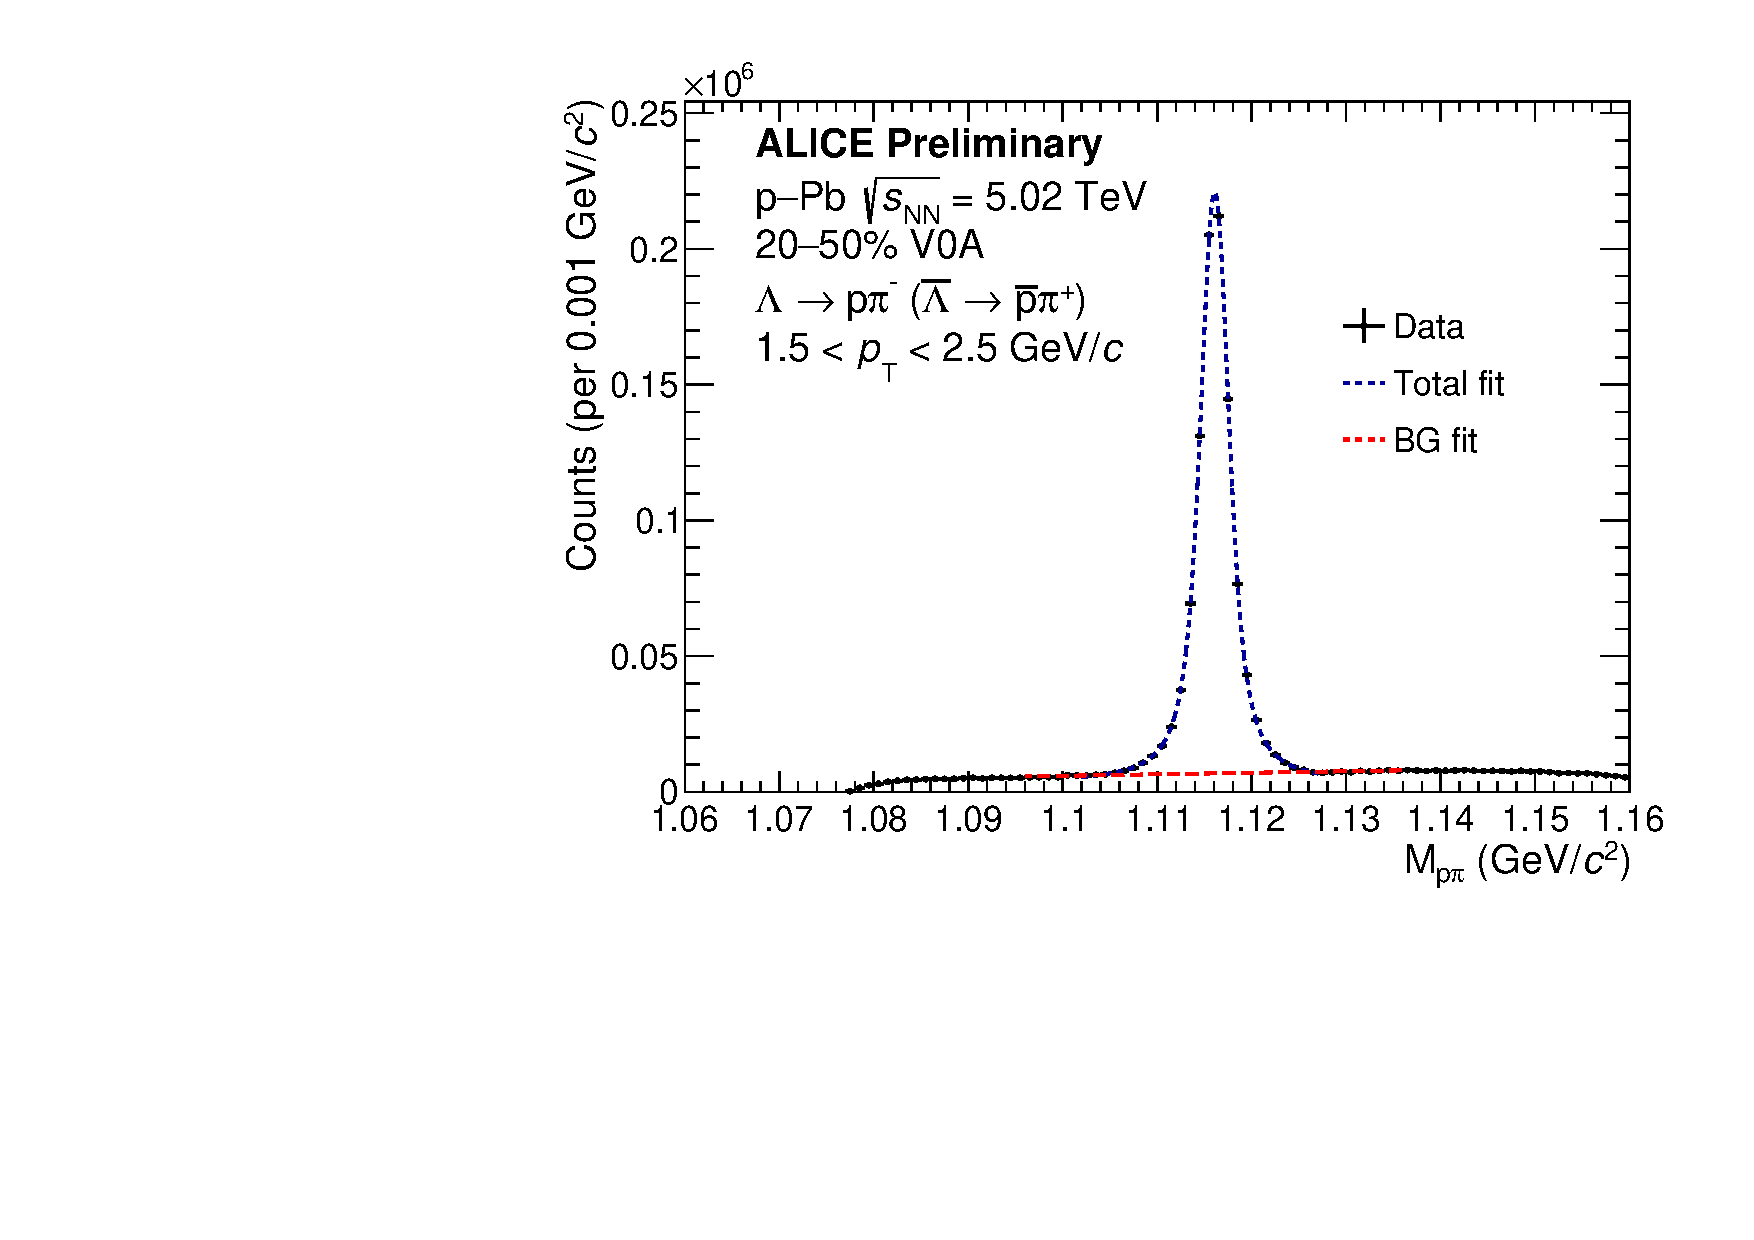
\includegraphics[width=\textwidth]{figures/analysis/lambda_mass_dist_20_50_lowpt.pdf}
	\end{minipage}
	\begin{minipage}{0.48\textwidth}
		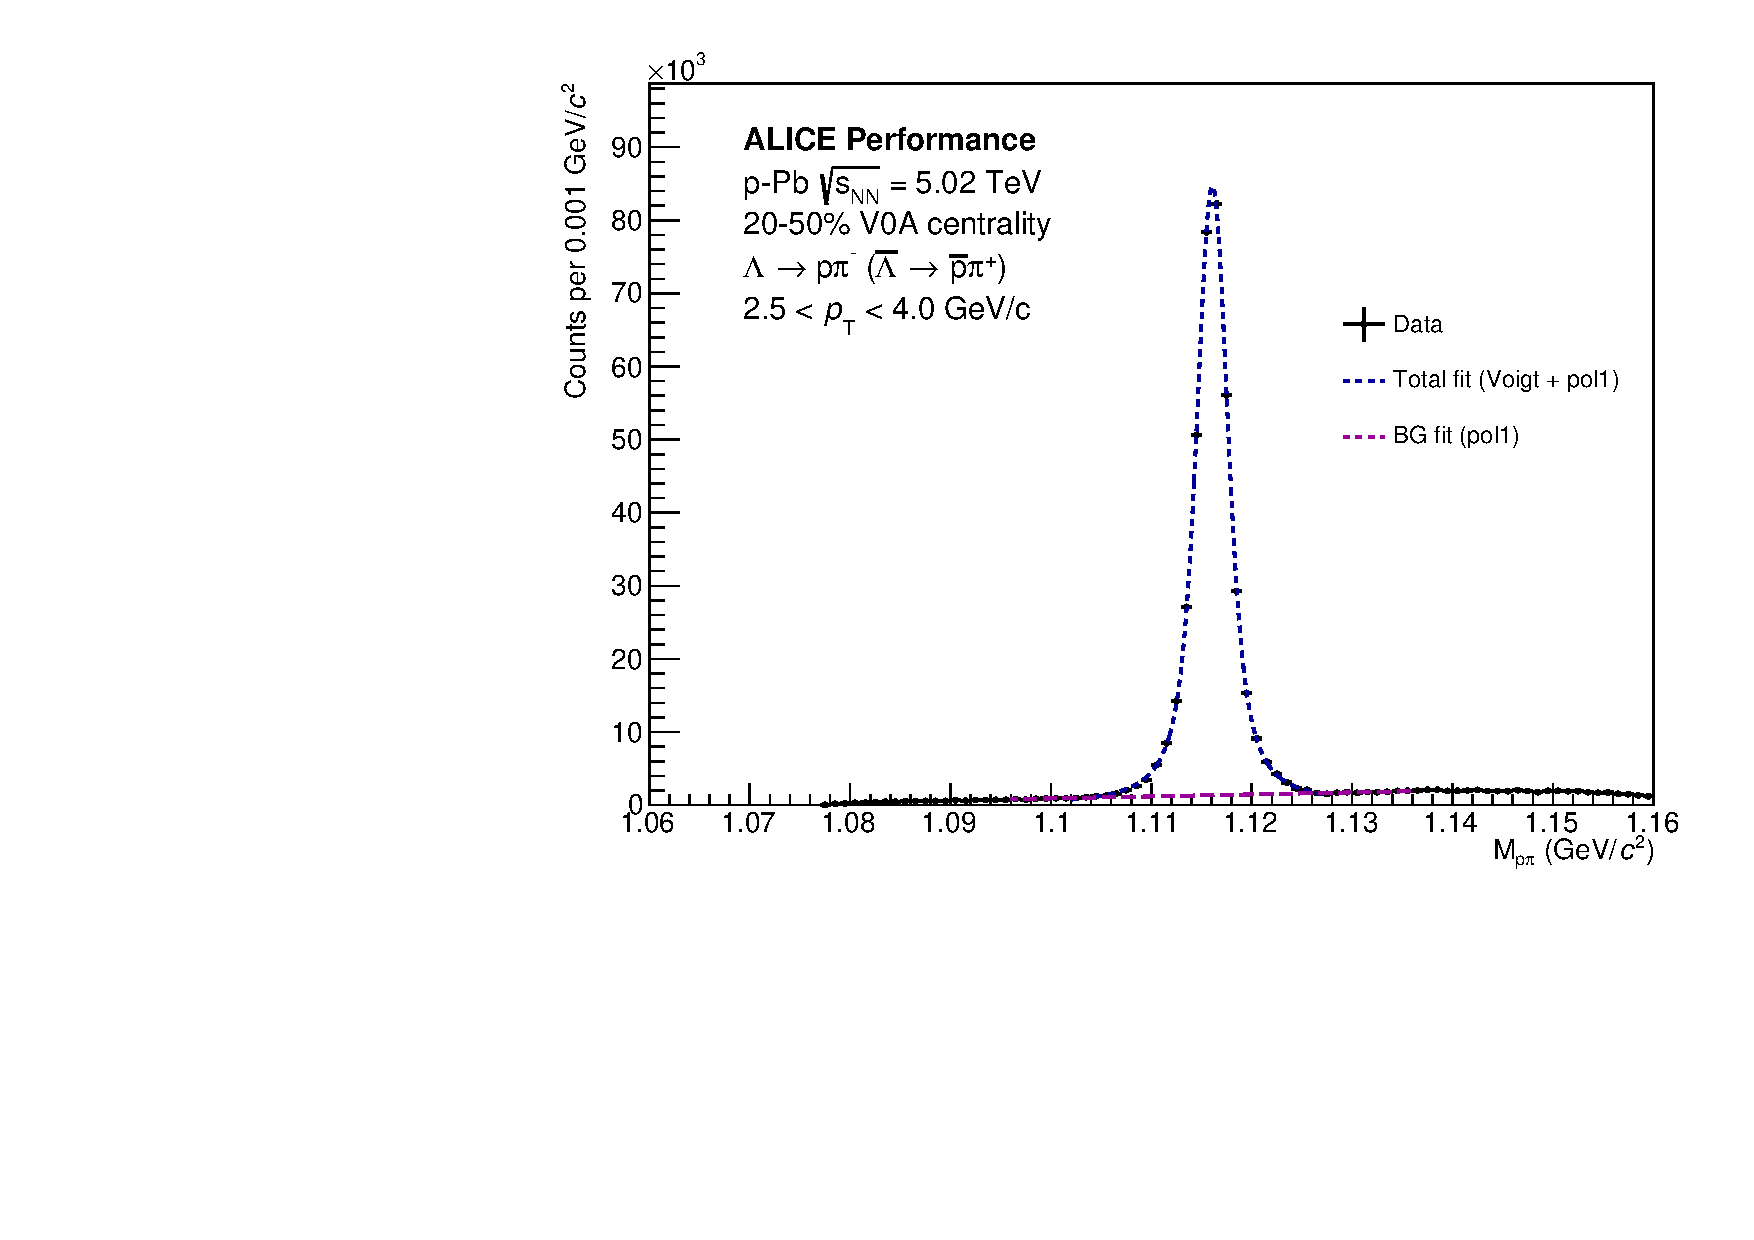
\includegraphics[width=\textwidth]{figures/analysis/lambda_mass_dist_20_50_highpt.pdf}
	\end{minipage}
	\begin{minipage}{0.48\textwidth}
		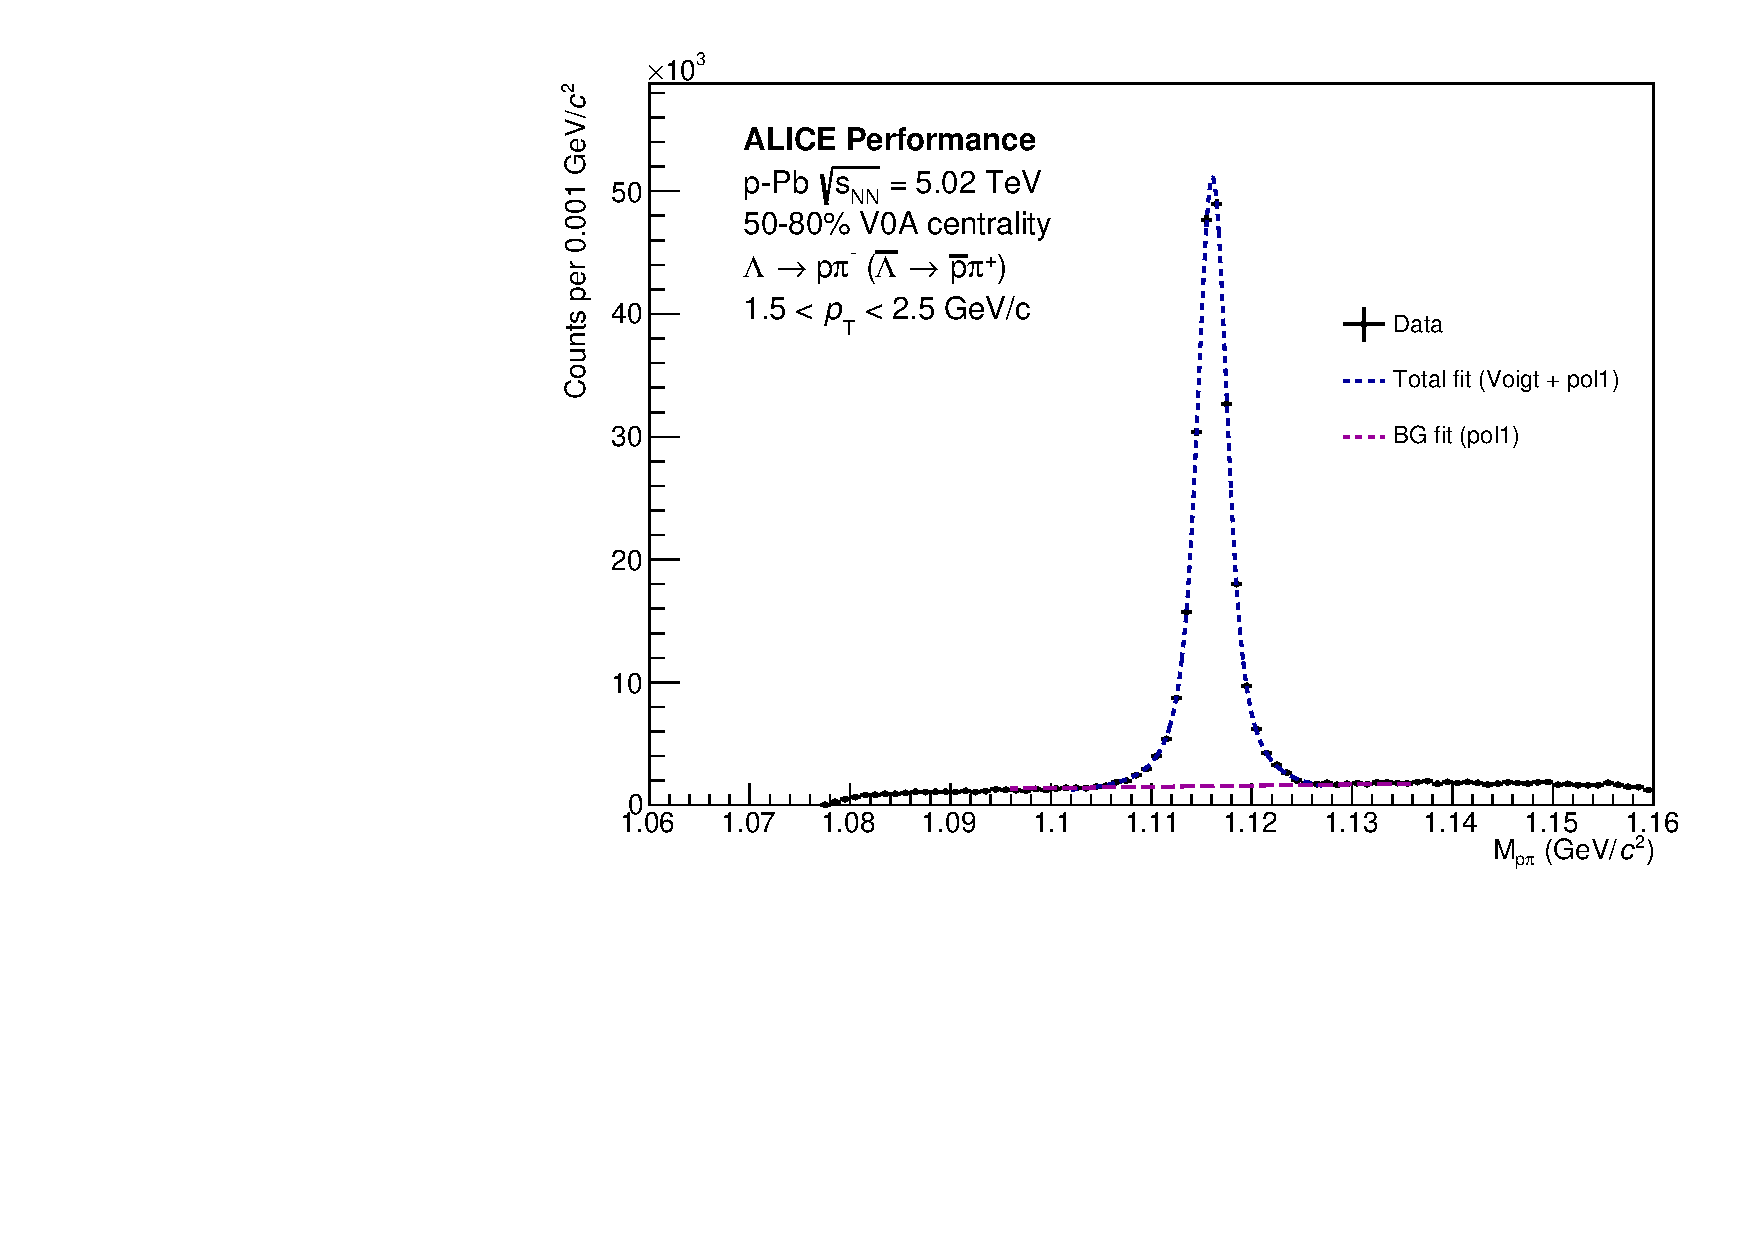
\includegraphics[width=\textwidth]{figures/analysis/lambda_mass_dist_50_80_lowpt.pdf}
	\end{minipage}
	\begin{minipage}{0.48\textwidth}
		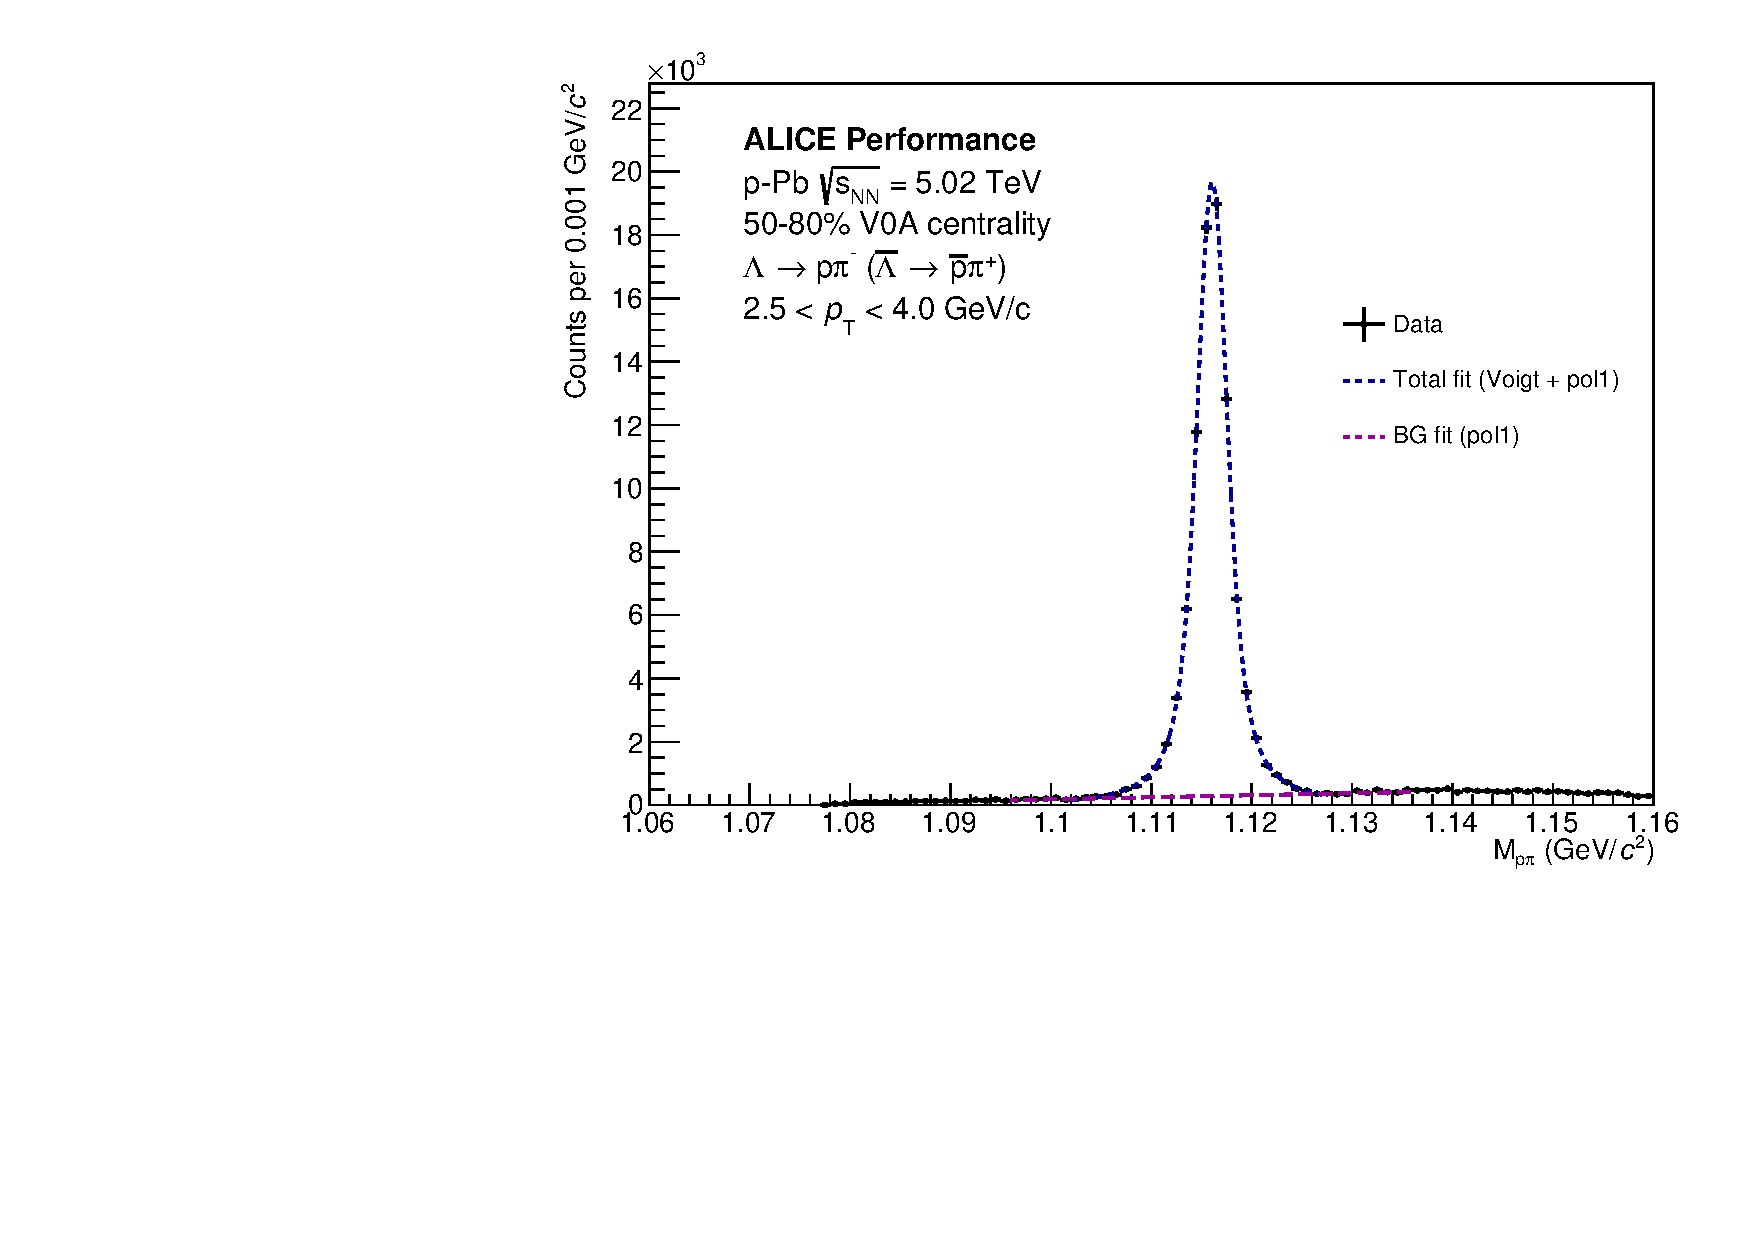
\includegraphics[width=\textwidth]{figures/analysis/lambda_mass_dist_50_80_highpt.pdf}
	\end{minipage}
	\caption{Invariant mass distributions in the 0-20\% (top), 20-50\% (middle), and 50-80\% (bottom) multiplicity bins for the $\Lambda$ candidates which pass the selection criteria with $1.5 < p_{\text{T}} < 2.5$ GeV/$c$ (left) and $2.5 < p_{\text{T}} < 4.0$ GeV/$c$ (right). A Voigtian signal + straight-line background fit to the data is shown in blue, with just the background fit shown in red. For these plots, the $\Lambda$s were only reconstructed in events with a trigger hadron.} 
	\label{fig:lambda_mass}
\end{figure}

\clearpage

\section{Reconstruction efficiency}
\label{sec:reconstruction_efficiency}

In an ideal world, the number of reconstructed particles of interest would be equal to the number of particles produced in the collision. Unfortunately, this is not the case in real data, as there are a number of detector effects which can cause particles to be ``lost'' during reconstruction. To correct for these effects, the reconstruction efficiency
%
\begin{equation}
	\epsilon(x_1, x_2, ..., x_n) \equiv P(f(x_1, x_2, ..., x_n) | g(x_1, x_2, ..., x_n)),
	\label{eq:efficiency_th}
\end{equation}
%
is used. Here $x_i$ are the kinematic variables of the particle of interest (e.g. \pt, $\eta$, $\varphi$), $f(x_1, x_2, ..., x_n)$ is the probability that a particle is reconstructed (``found'') with kinematic variables $x_i$, and $g(x_1, x_2, ..., x_n)$ is the probability that a particle is produced (``generated'') with the same variables. While the distributions $f$ and $g$ are inaccessable within a given event, the efficiency can be calculated using Monte Carlo simulation techniques via the equation
%
\begin{equation}
	\epsilon(x_1, x_2, ..., x_n) = \frac{N_{\text{reco.}}(x_1, x_2, ..., x_n)}{N_{\text{gen.}}(x_1, x_2, ..., x_n)},
	\label{eq:efficiency_exp}
\end{equation}
%
where $N_{\text{reco.}}$ and $N_{\text{gen.}}$ are the reconstructed and generated particle distributions, respectively, usually taken across a large number of simulated events. In this analysis, these distributions are calculated as a function of \pt and $\eta$ for each multiplicity class using 30 million events generated by the Monte Carlo event generator DPMJET~\cite{DPMJET} with particle propagation through the ALICE detector simulated by the GEANT3~\cite{GEANT} detector simulation software. These efficiency distributions are then used to correct the h-$\Lambda$ and h-h correlation distributions using the procedure described in Section~\ref{sec:corrections}.

\subsection{Charged hadron reconstruction efficiency}

The trigger and associated hadron track reconstruction efficiencies are calculated using Equation~\ref{eq:efficiency_exp}, where the trigger and associated hadrons from $N_{\text{reco.}}$ are subject to the following constraints:
%
\begin{itemize}
	\item The track passes the quality cuts outlined in Tables~\ref{tab:trigger_track_cuts} (trigger) or \ref{tab:primary_track_cuts} (associated)
	\item The track has a corresponding generated particle
	\item That generated particle is either a pion, proton, kaon, electron, or muon
	\item $|\eta_{\text{track}}| \leq 0.8$,
\end{itemize}
%
and the trigger and associated hadrons from $N_{\text{gen.}}$ are subject to:
%
\begin{itemize}
	\item $|\eta_{\text{track}}| \leq 0.8$
	\item The particle is either a pion, proton, kaon, electron, or muon
	\item The particle is primary (i.e. did not originate from a weak decay)
\end{itemize}
%
The trigger and associated track reconstruction efficiencies are shown for each multiplicity class as a function of \pt in Figure~\ref{fig:trigassoc_eff_pt}. While these efficiencies exhibit relatively flat behavior as a function of \pt and multiplicity, they are still treated as \pt and multiplicity dependent during the correction procedure.

\begin{figure}[h]
	\centering
	\begin{minipage}{0.48\textwidth}
		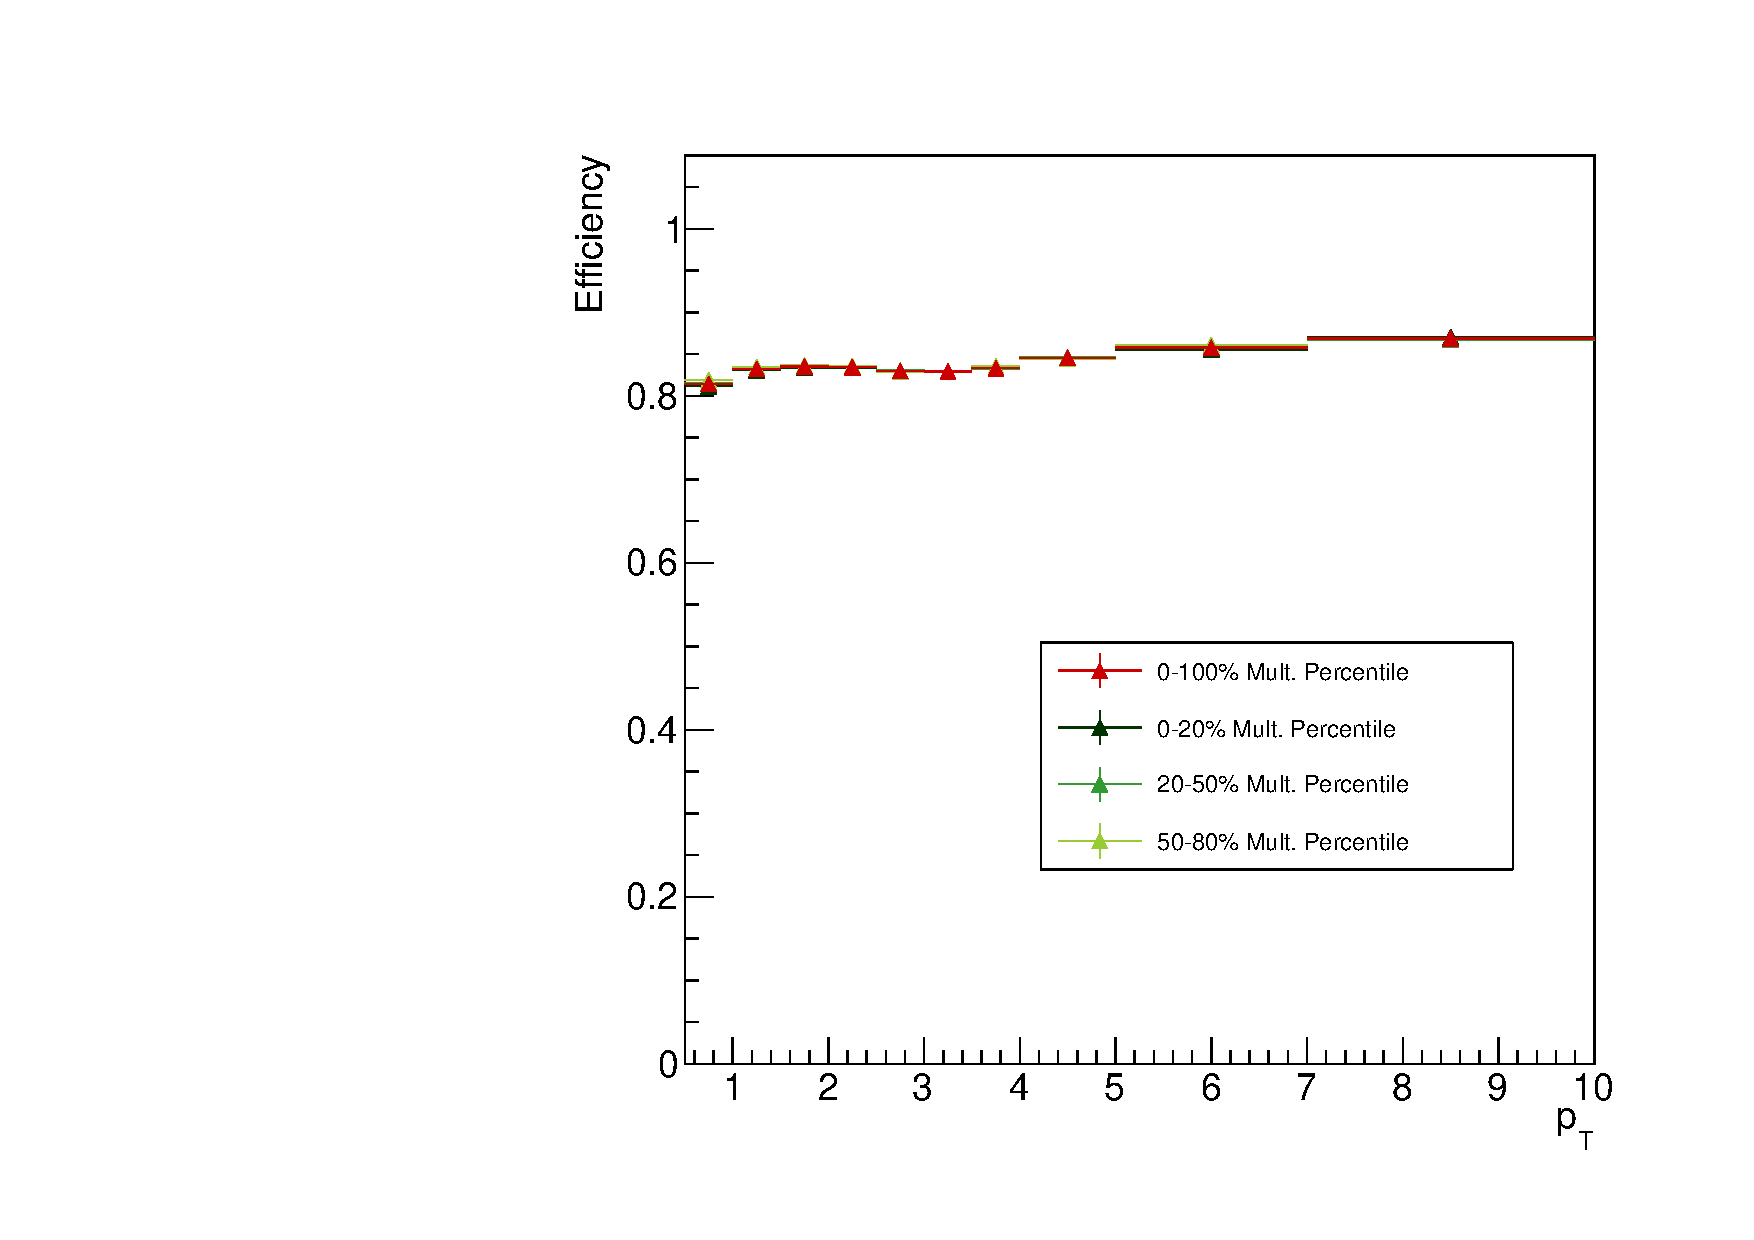
\includegraphics[width=\textwidth]{figures/analysis/trigger_efficiency.pdf}
	\end{minipage}
	\begin{minipage}{0.48\textwidth}
		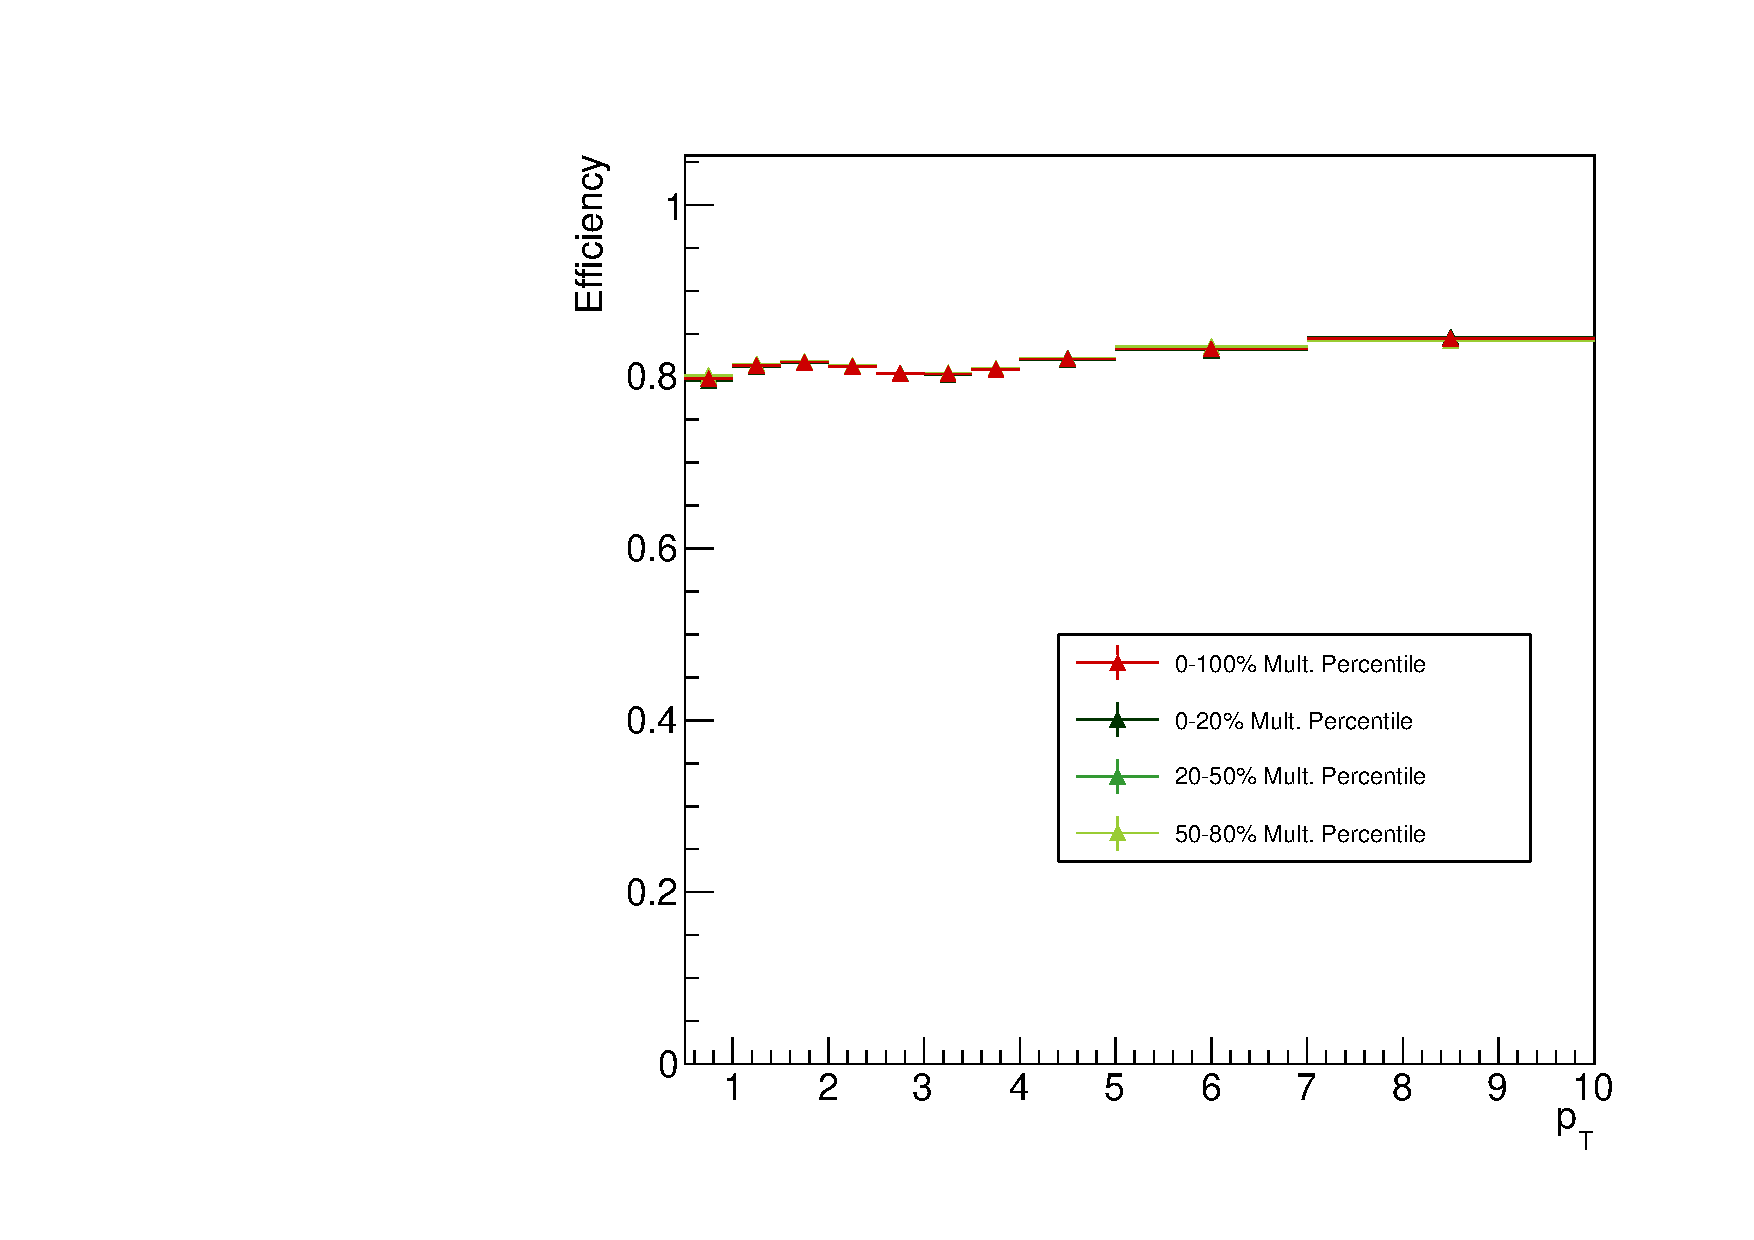
\includegraphics[width=\textwidth]{figures/analysis/associated_efficiency.pdf}
	\end{minipage}
	\caption{Efficiency vs. $p_T$ for trigger (left) and associated (right) hadrons. While the values are similar, the associated hadron efficiency is slightly lower due to the stricter selection criteria.}
	\label{fig:trigassoc_eff_pt}
\end{figure}

\subsection{$\Lambda$ reconstruction efficiency}

 The $\Lambda$ reconstruction efficiency is calculated as a function of \pt and $\eta$ using Equation~\ref{eq:efficiency_exp}, where the $\Lambda$s from $N_{\text{reco.}}$ are subject to the following conditions:
%
\begin{itemize}
	\item They pass the topological selection criteria from Table~\ref{tab:lambda_selection}
	\item The reconstructed daughter p, $\pi$ tracks pass the quality cuts from Table~\ref{tab:lambda_daughter_track_cuts}
	\item The daughter p, $\pi$ tracks have corresponding generated p, $\pi$ particles
	\item Those generated p, $\pi$ daughters come from the same mother $\Lambda$
	\item $|\eta_{\Lambda}| \leq 0.8$,
\end{itemize}
%
and the $\Lambda$s from $N_{\text{gen.}}$ are subject to:
%
\begin{itemize}
	\item $|\eta_{\Lambda}| \leq 0.8$
	\item The $\Lambda$ decays to p$\pi$.
\end{itemize}
%
The requirement that the generated $\Lambda$s decay into p$\pi$ means the branching ratio is not included in the efficiency calculation and therefore is corrected for separately (see Section \ref{sec:corrections}). The $\Lambda$ reconstruction efficiency can be seen for each multiplicity class as a function of \pt and $\eta$ in Figure~\ref{fig:lambda_eff}. Note that the efficiency is no longer flat as a function of $\eta$ due to the $|\eta| < 0.8$ requirement for the daughter tracks, which kinematically restricts the reconstructed $\Lambda$ to a smaller $\eta$ range.

\begin{figure}[h]
	\centering
	\begin{minipage}{0.48\textwidth}
		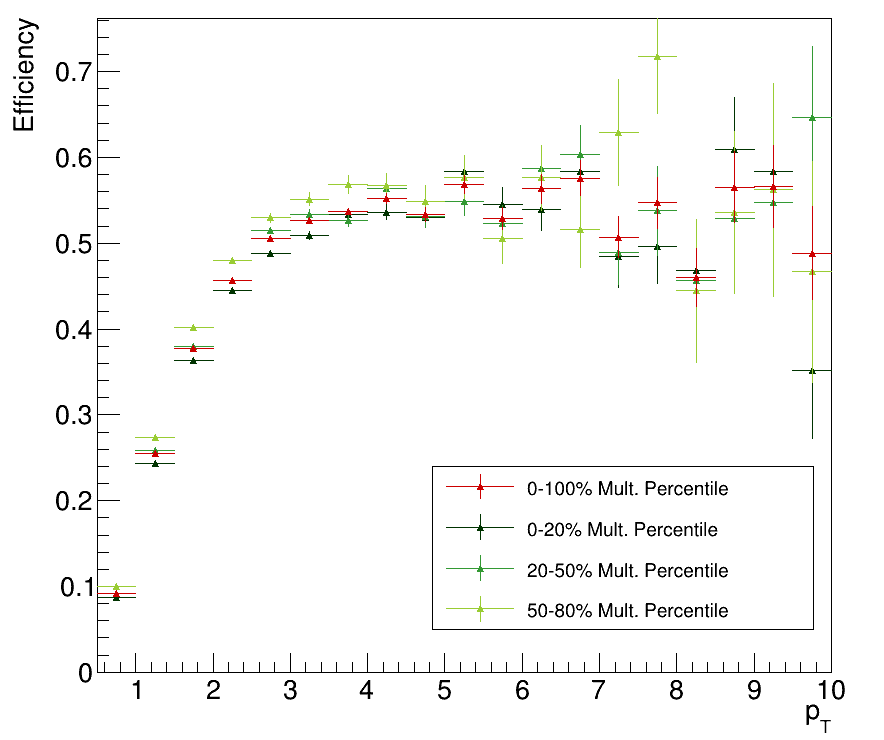
\includegraphics[width=\textwidth]{figures/analysis/v0_efficiency_pt.png}
	\end{minipage}
	\begin{minipage}{0.48\textwidth}
		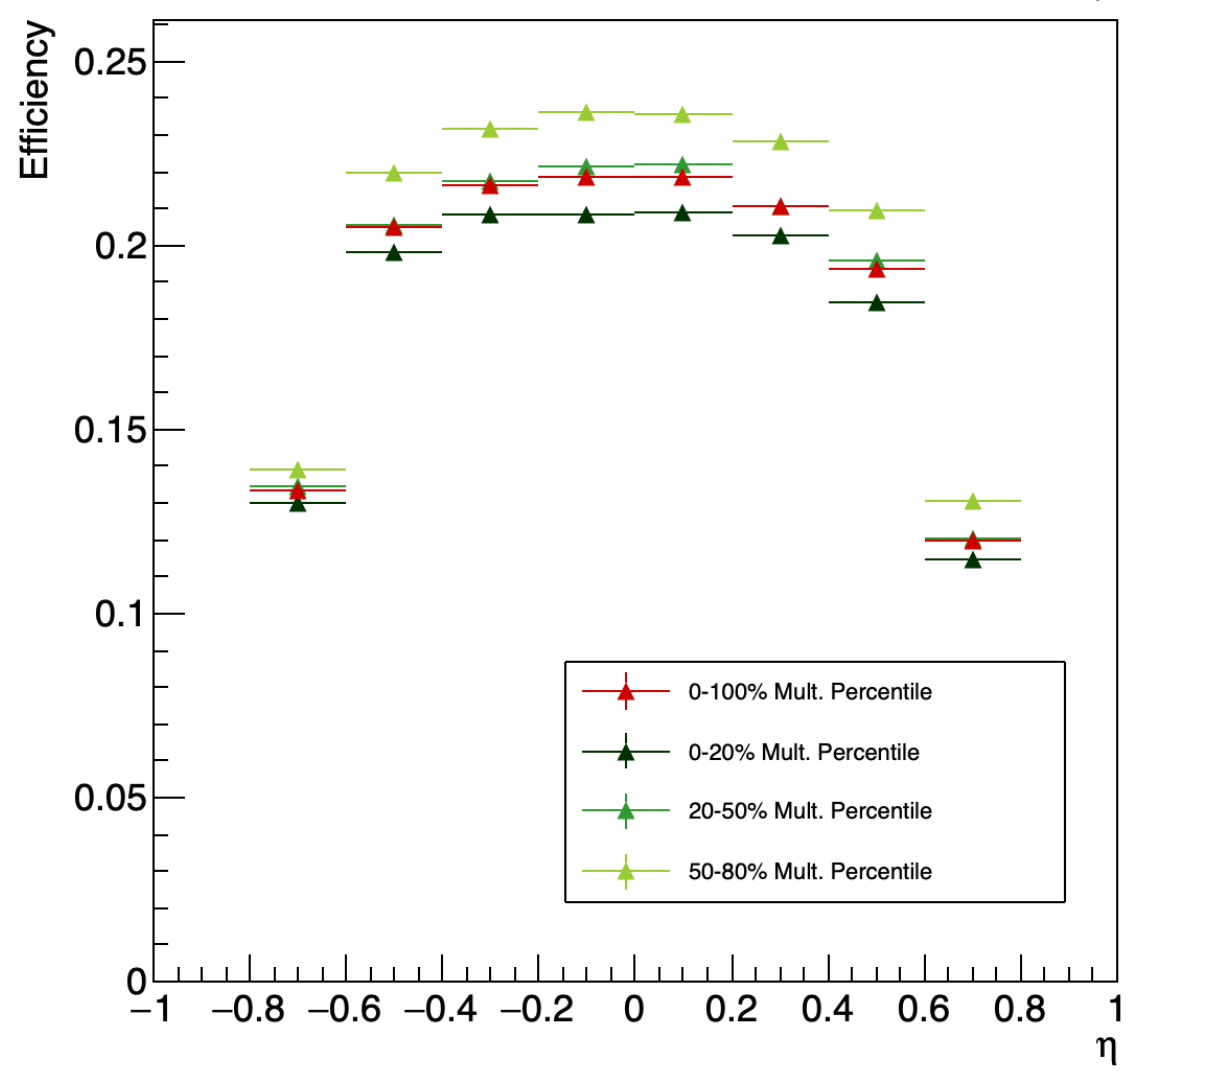
\includegraphics[width=\textwidth]{figures/analysis/v0_efficiency_eta.png}
	\end{minipage}
	\caption{Efficiency vs. $p_T$ (left) and $\eta$ (right) for $\Lambda$ reconstruction in each multiplicty bin, along with an integrated 0-100\% point in red.}
	\label{fig:lambda_eff}
\end{figure}

\clearpage 

\section{Corrections to the correlation distributions}
\label{sec:corrections}

Once the trigger and associated particles are selected, the two-particle h-$\Lambda$ and h-h correlation distributions are generated. As mentioned in the previous chapter, the corrected two-particle correlation function is given by
%
\begin{equation}
    \frac{1}{N_{trig}}\frac{d^2N_{pair}}{d\Delta\varphi d\Delta\eta} = \frac{1}{N_{trig}^{corr}}\frac{1}{\epsilon_{trig}\times\epsilon_{assoc}}B(0,0)\frac{S(\Delta\varphi, \Delta\eta)}{B(\Delta\varphi, \Delta\eta)}.
\label{eq:corr_detector_ref}
\end{equation}
%
which contains a number of explicit correction terms (in the form of $\epsilon$s) along with some implicit corrections. These corrections are described in this section, and are presented in the order in which they are applied to the data.

\subsection{Single-particle efficiency corrections}
\label{sec:single_particle_corr}

As both the trigger and the associated particles have their own independent reconstruction efficiencies, the trigger-associated pair reconstruction efficiency should be
%
\begin{equation}
	\epsilon_{\text{trig}, \text{assoc}} = \epsilon_{\text{trig}}\times\epsilon_{\text{assoc}},
\end{equation} 
%
meaning the single-particle efficiency distributions from Section \ref{sec:reconstruction_efficiency} can be used to calculate the weight $1/(\epsilon_{trig}\times\epsilon_{assoc})$. This weight is applied for each h-$\Lambda$ and h-h pair in the two-dimensional correlation distribution. However, the assumption that the reconstruction efficiencies are independent is slightly incorrect in the case of the h-$\Lambda$ distributions due to track merging effects, thus an additional $\epsilon_{pair}$ correction is required (discussed in detail in Section~\ref{sec:lambda_corrections}).

The trigger efficiency weight $1/\epsilon_{trig}$ is also applied to the single-particle trigger hadron distribution in data to obtain $N_{trig}^{corr}$. 

\subsection{Mixed-event acceptance correction}
\label{sec:acceptance_corr}

As mentioned in Section~\ref{sec:raw_corr}, the $B(0, 0)/B(\Delta\varphi, \Delta\eta)$ term in Equation \ref{eq:corr_detector} corrects for the finite acceptance along $\eta$ as both our trigger and associated particles are required to be within $|\eta| < 0.8$. The mixed-event distribution $B(\Delta\varphi, \Delta\eta)$ shown in Figure \ref{fig:twod_cor} has a characteristic triangular shape along $\Delta\eta$, which is purely due to detector geometry, as no physical correlations are present by construction. When scaled by 1/$B(0, 0)$, the mixed event distribution becomes the probability that a particle pair is found given that the trigger particle is within $|\eta| < 0.8$, which is unity at $\Delta\varphi, \Delta\eta$ = $0, 0$. Thus correcting the same-event distribution $S(\Delta\varphi, \Delta\eta)$ by $B(0, 0)/B(\Delta\varphi, \Delta\eta)$ removes this acceptance effect and allows for a more accurate determination of the pair-wise yields. 

While the generation of the mixed event distribution $B(\Delta\varphi, \Delta\eta)$ was discussed briefly in Section~\ref{sec:raw_corr}, the specific details are as follows. First, in order to ensure that the mixed-event pairs are coming from similar events, the events in the mixing pool are separated by both multiplicity percentile and $Z_{\text{vtx.}}$ position. The categorizing of events based off of $Z_{\text{vtx.}}$ position is an integral part of the acceptance correction: events with a $Z_{\text{vtx.}}$ at one edge of the detector have a completely different (and nearly inverted) $\eta$ acceptance than those on the opposite edge. The multiplicity bins are the same as they are for the same-event distributions (namely 0-20\%, 20-50\% and 50-80\%), and the ten $Z_{\text{vtx.}}$ bins are split evenly from -10 cm to 10 cm.  For each multiplicity and $Z_{\text{vtx.}}$ bin, the acceptance correction
%
\begin{equation}
	S_{\text{corr.}}(\Delta\varphi, \Delta\eta) = \frac{S(\Delta\varphi, \Delta\eta)}{B(\Delta\varphi, \Delta\eta)/B(0, 0)}
\end{equation}
%
is performed, and the results for each multiplicity bin are then merged across all $Z_{\text{vtx.}}$ bins. The uncorrected distributions $S(\Delta\varphi, \Delta\eta)$ and the mixed-event distributions $B(\Delta\varphi, \Delta\eta)$ are shown for both the h-$\Lambda$ and h-h cases for all multiplicity and associated momentum bins in Figures~\ref{fig:h_lambda_2d_nomixcor} through~\ref{fig:h_h_2d_mixed}.


\begin{figure}[ht]
	\centering
	\begin{minipage}{0.48\textwidth}
		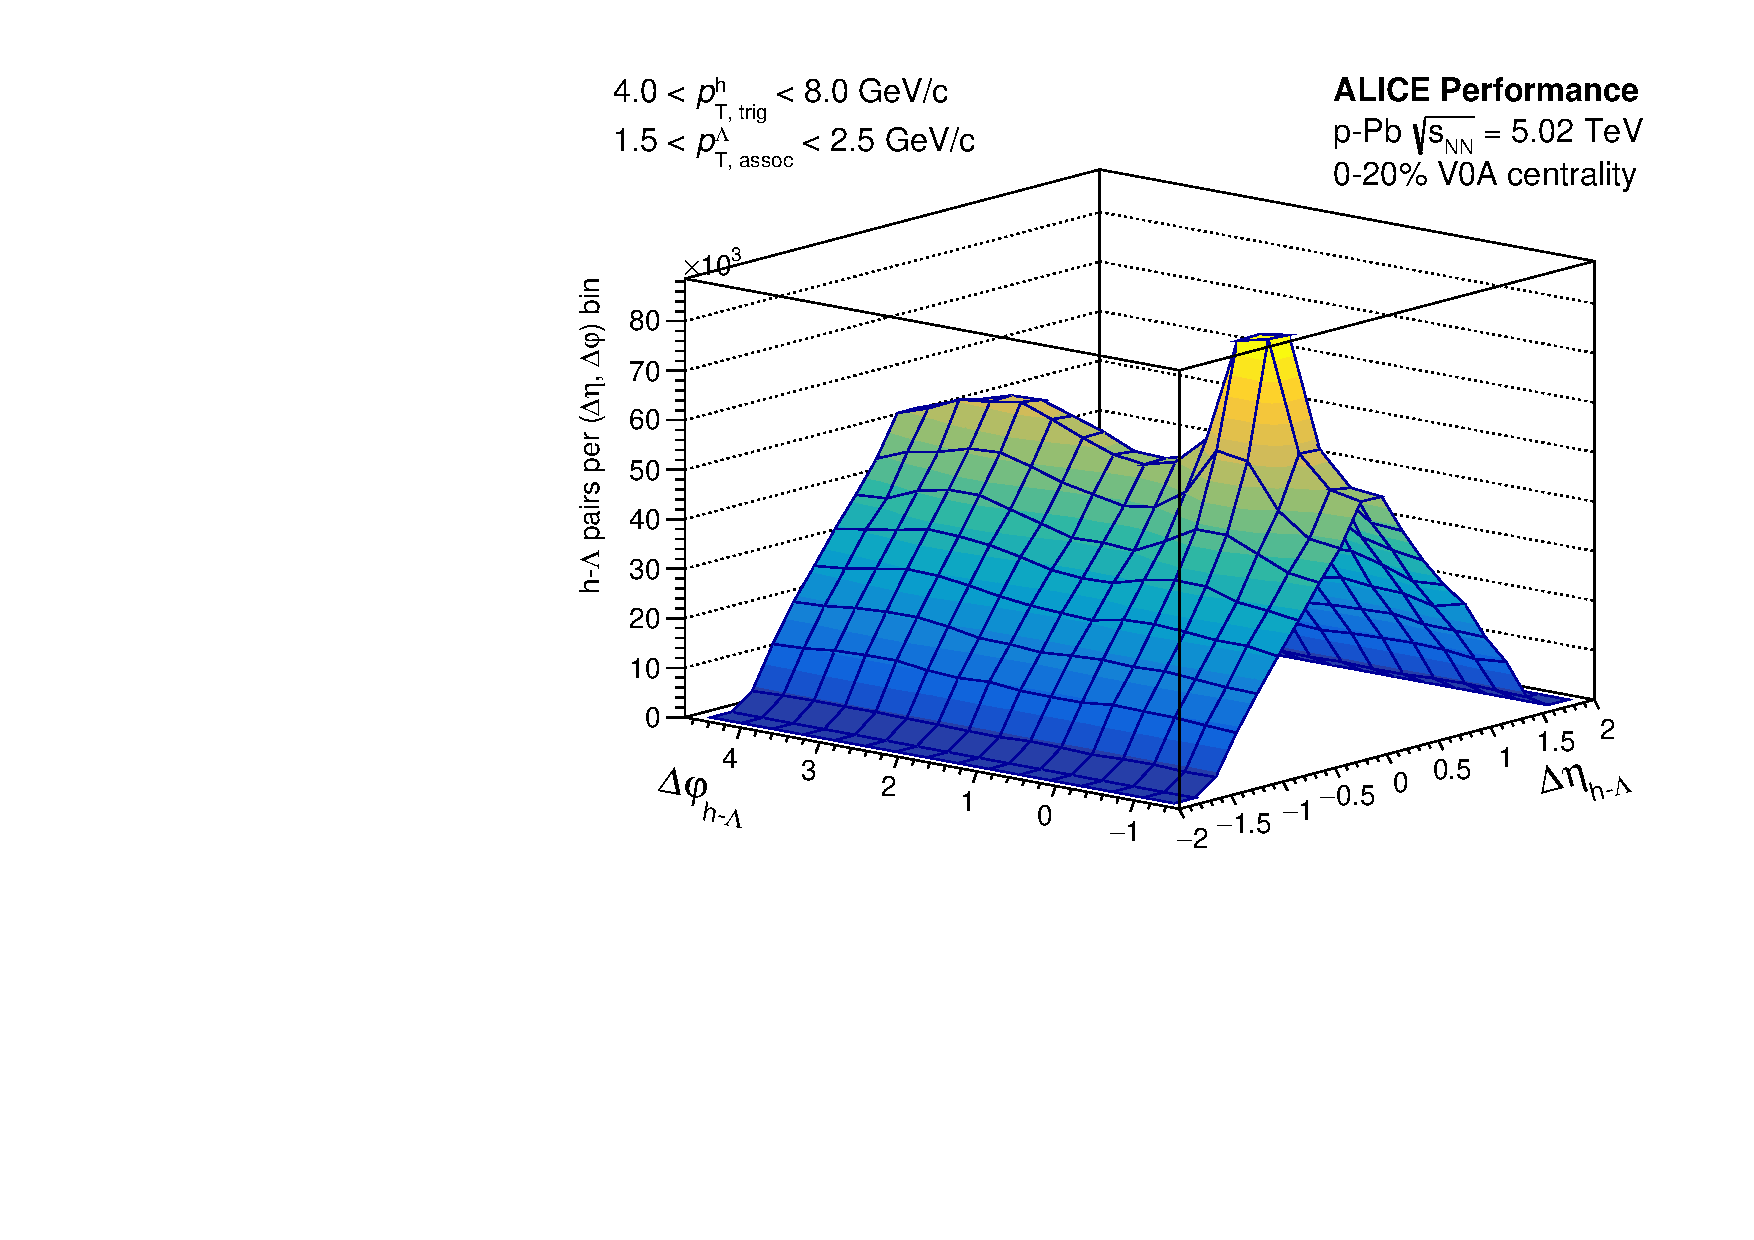
\includegraphics[width=\textwidth]{figures/analysis/h_lambda_2d_nomixcor_fancy_label_0_20_lowpt.pdf}
	\end{minipage}
	\begin{minipage}{0.48\textwidth}
		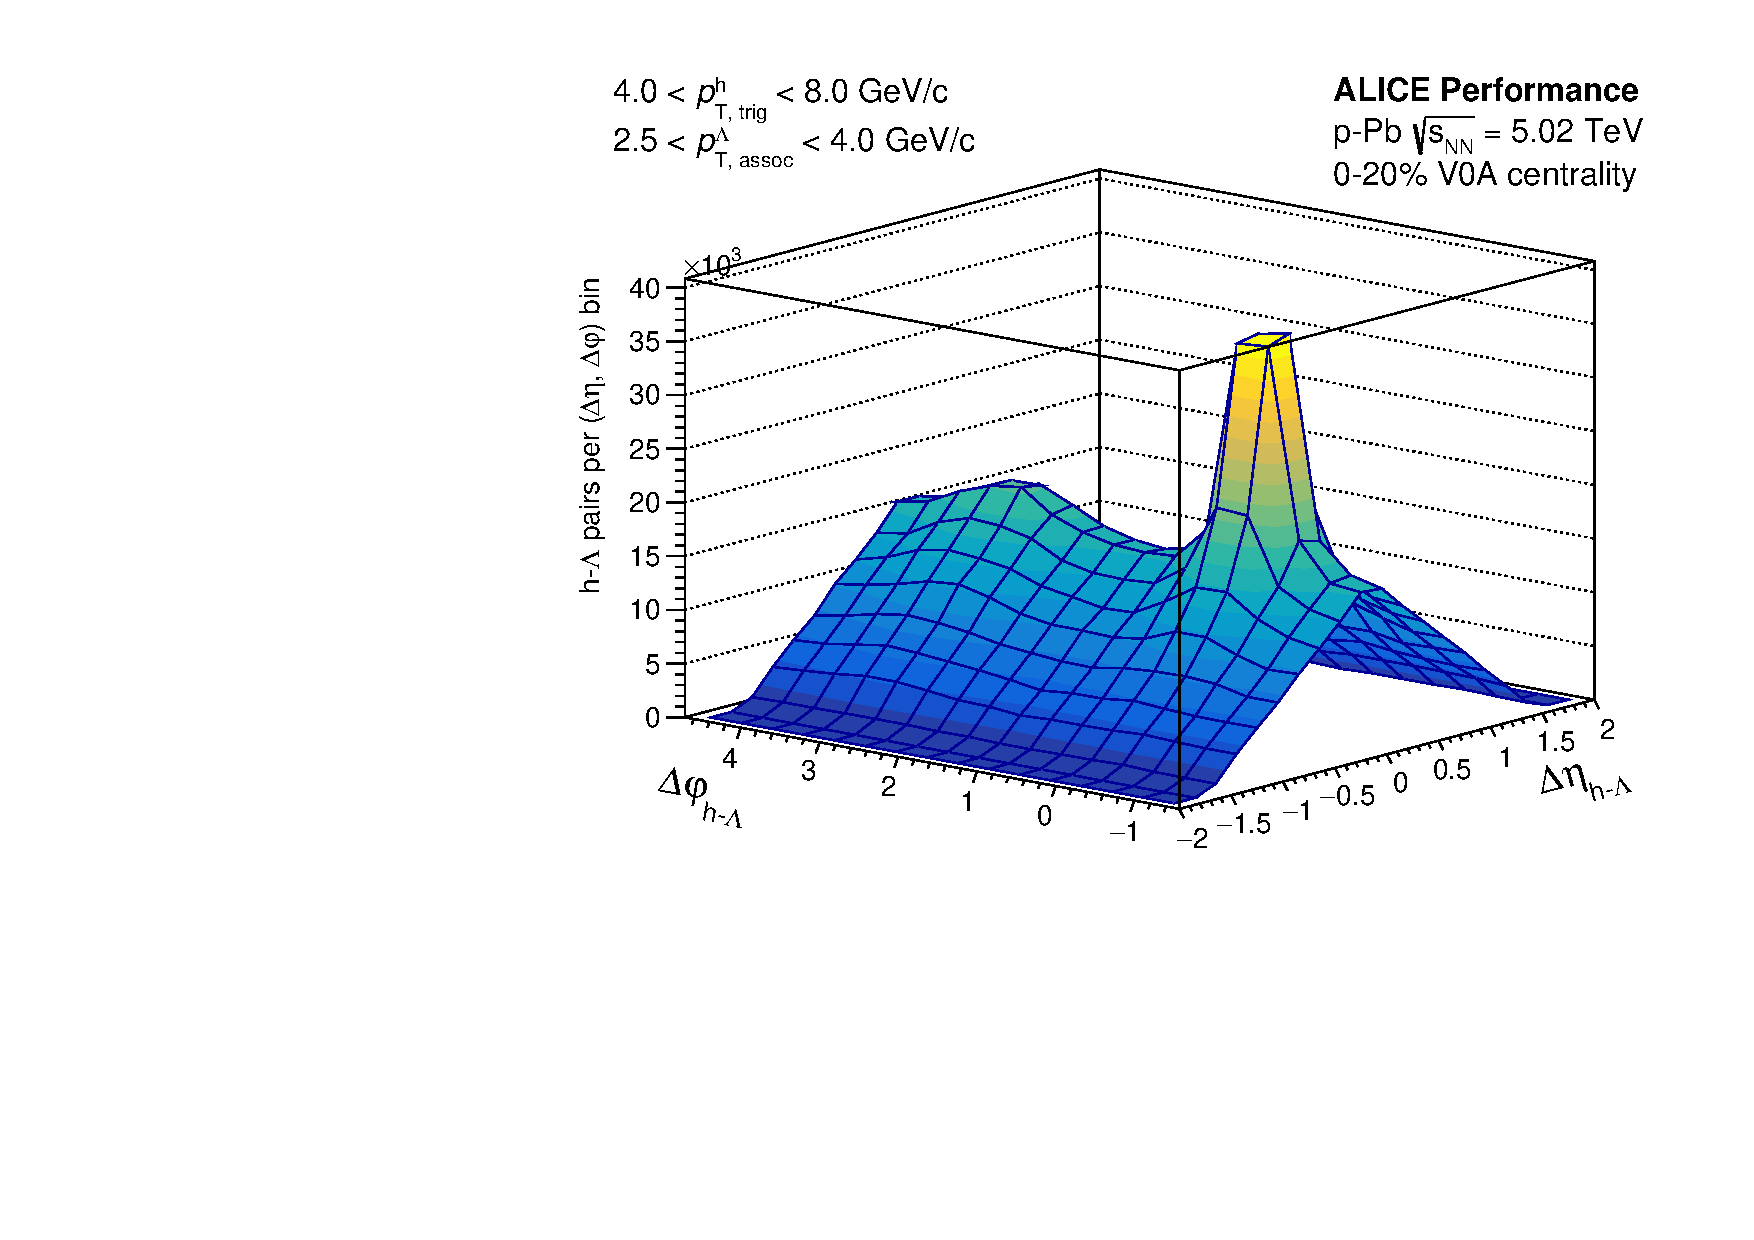
\includegraphics[width=\textwidth]{figures/analysis/h_lambda_2d_nomixcor_fancy_label_0_20_highpt.pdf}
	\end{minipage}
	\begin{minipage}{0.48\textwidth}
		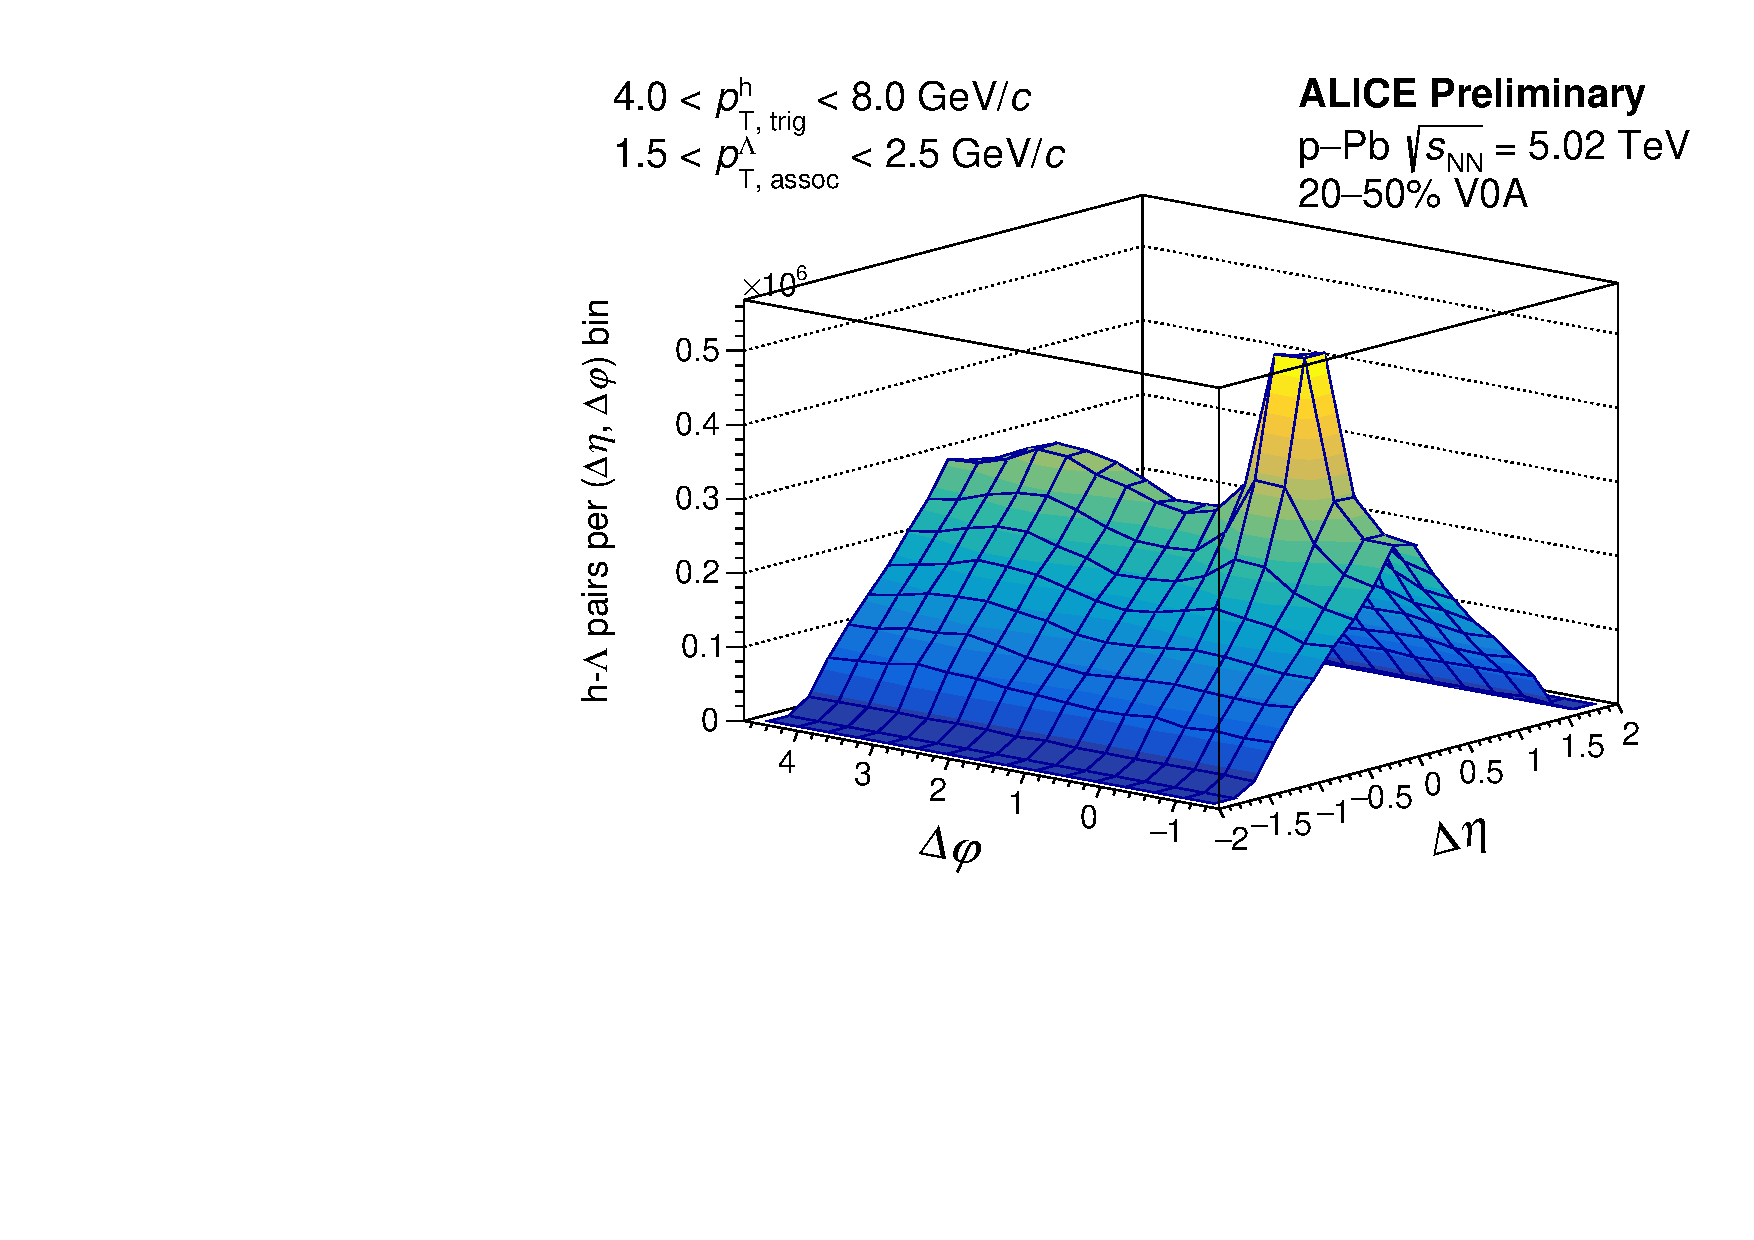
\includegraphics[width=\textwidth]{figures/analysis/h_lambda_2d_nomixcor_fancy_label_20_50_lowpt.pdf}
	\end{minipage}
	\begin{minipage}{0.48\textwidth}
		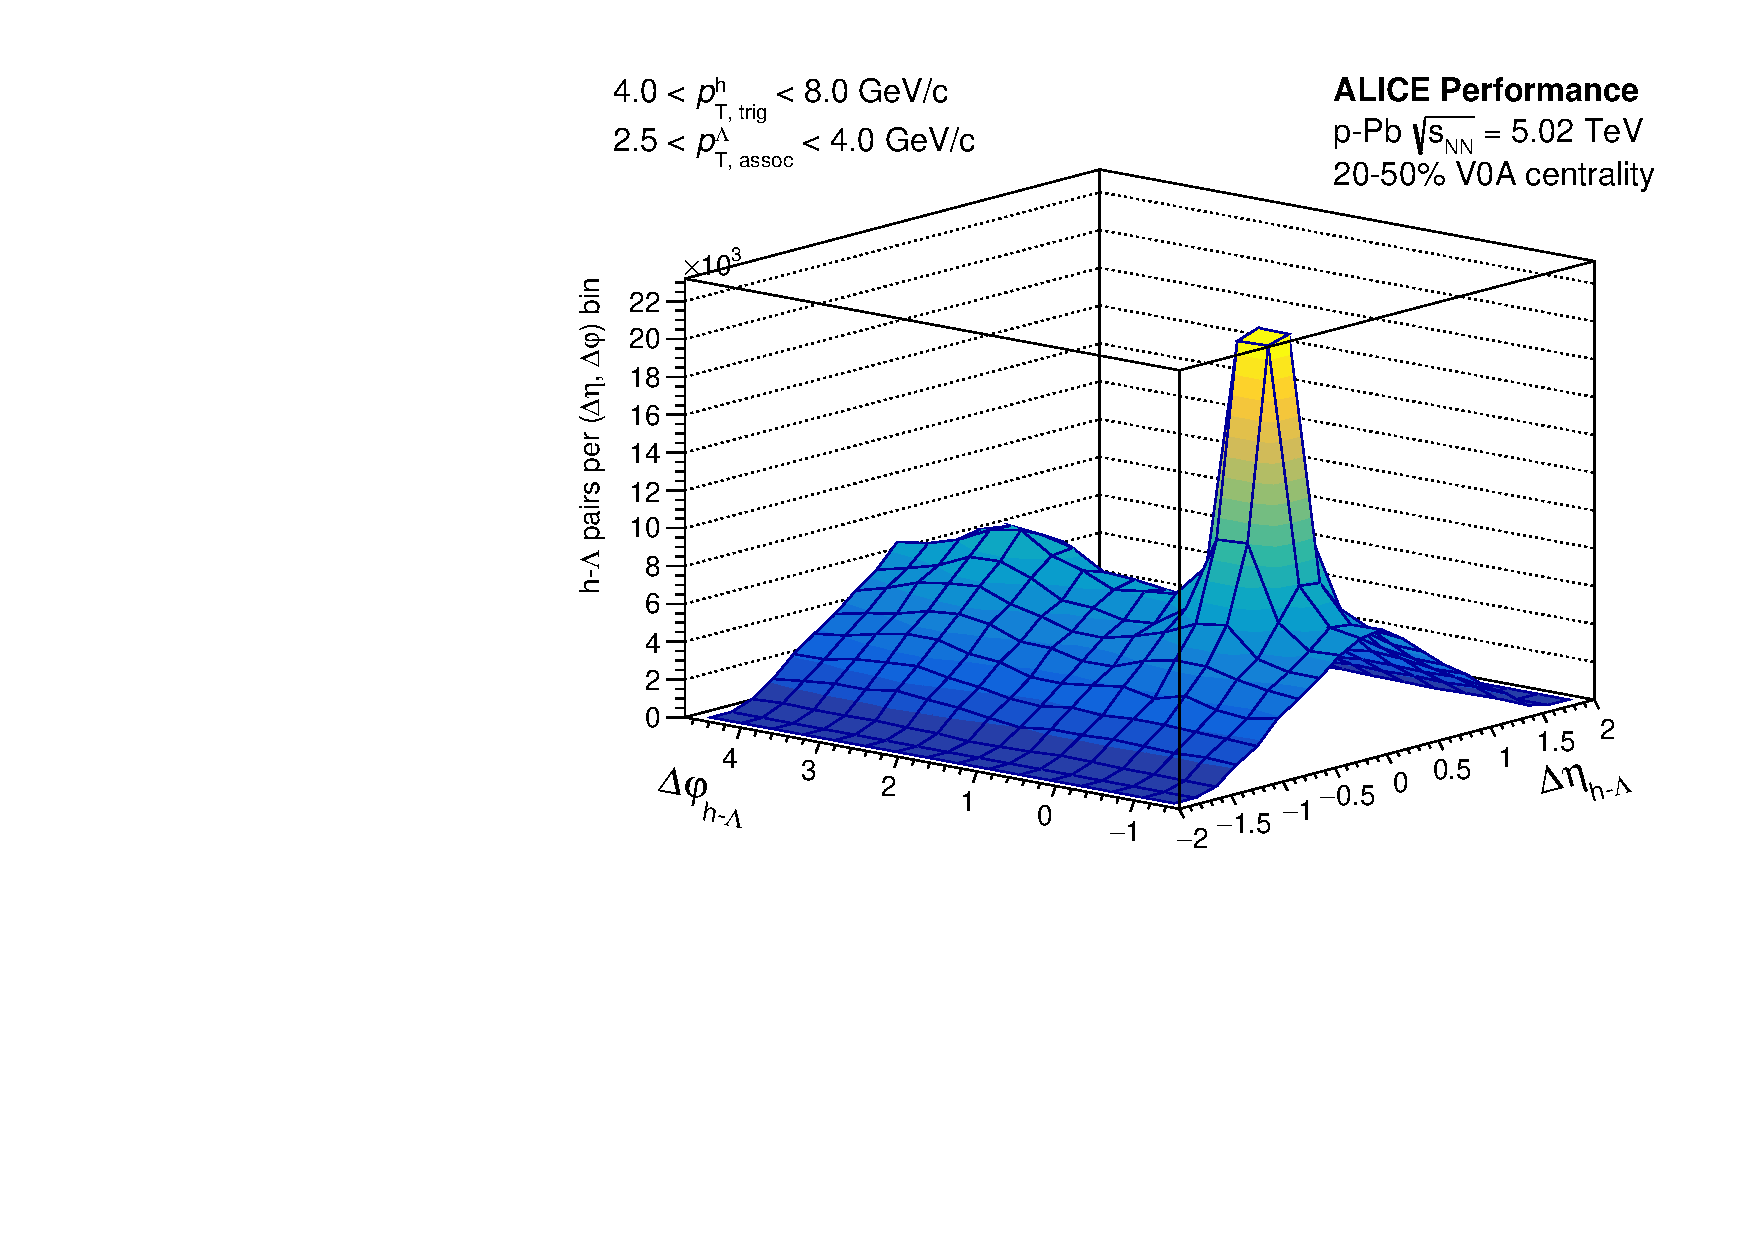
\includegraphics[width=\textwidth]{figures/analysis/h_lambda_2d_nomixcor_fancy_label_20_50_highpt.pdf}
	\end{minipage}
	\begin{minipage}{0.48\textwidth}
		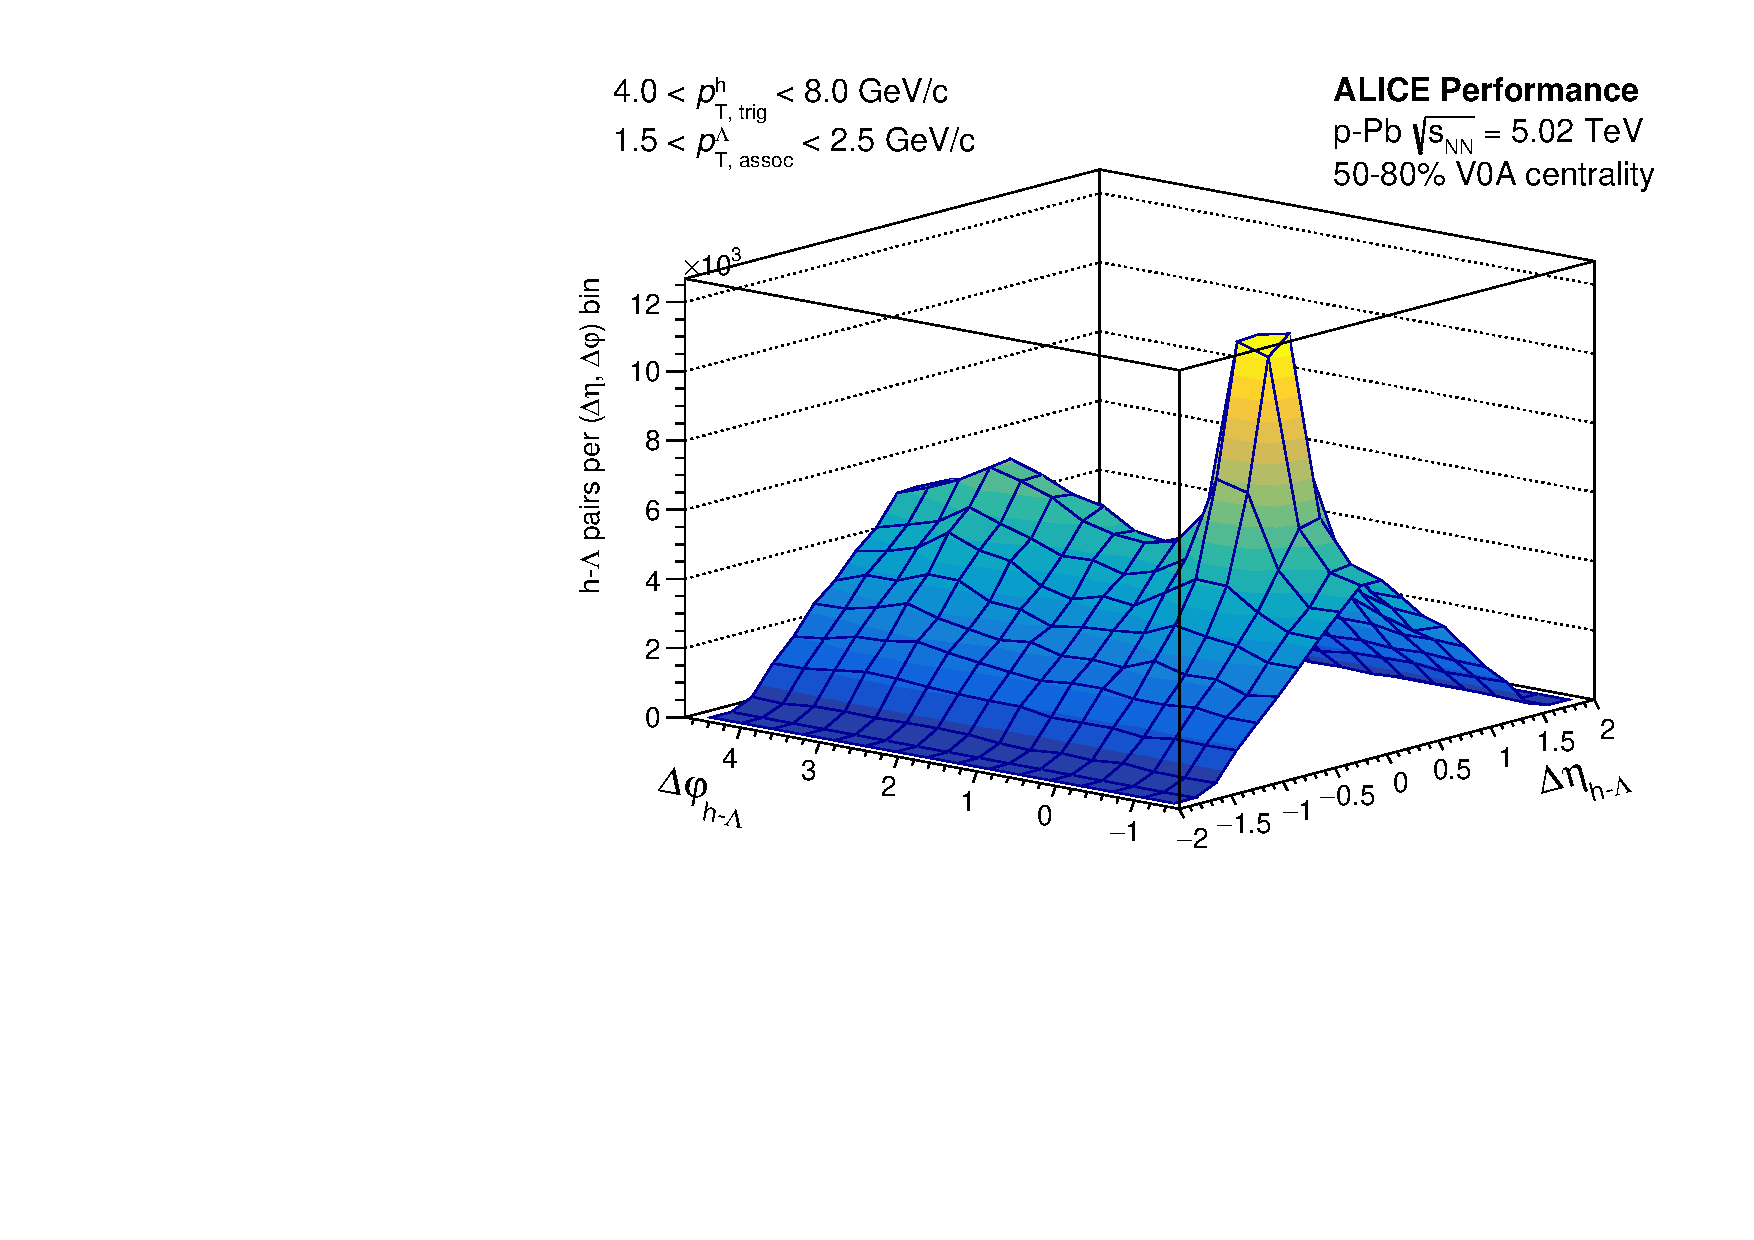
\includegraphics[width=\textwidth]{figures/analysis/h_lambda_2d_nomixcor_fancy_label_50_80_lowpt.pdf}
	\end{minipage}
	\begin{minipage}{0.48\textwidth}
		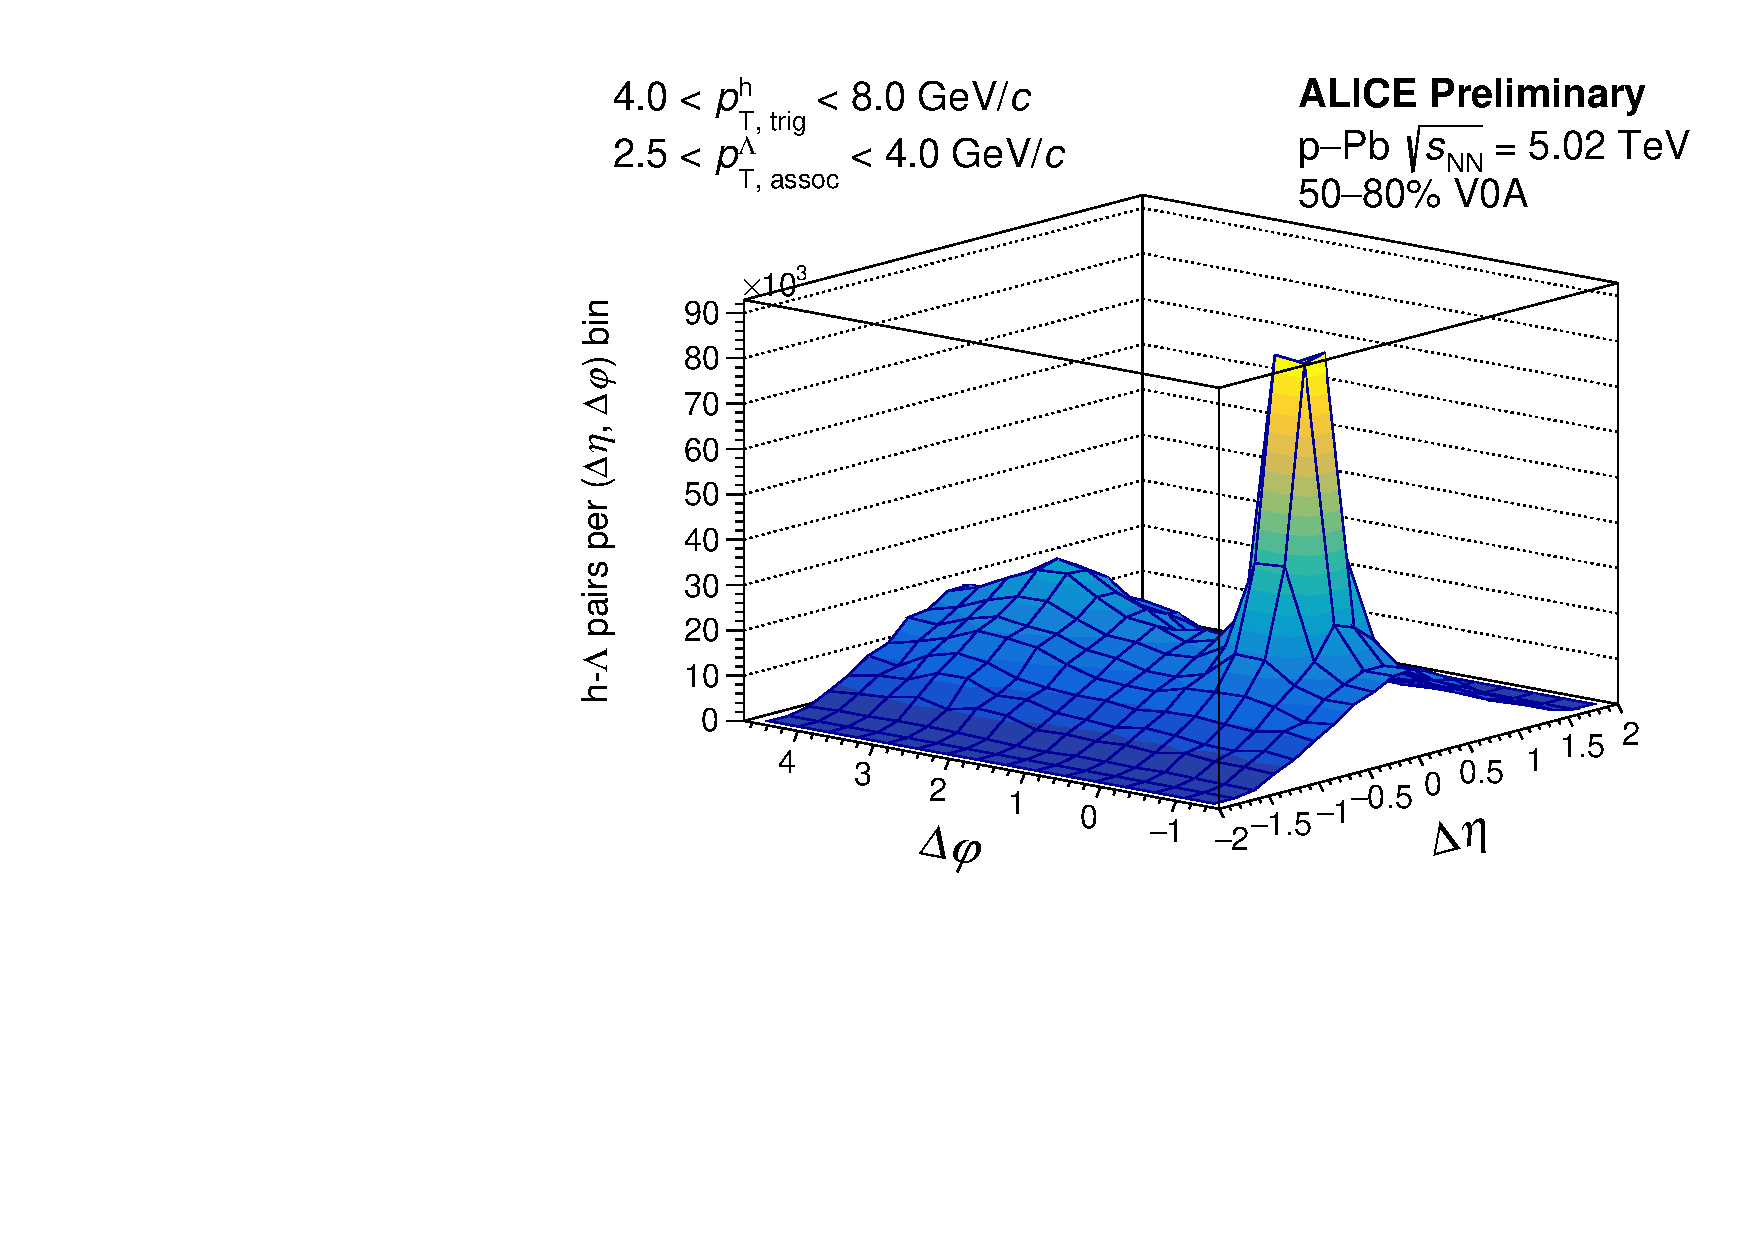
\includegraphics[width=\textwidth]{figures/analysis/h_lambda_2d_nomixcor_fancy_label_50_80_highpt.pdf}
	\end{minipage}
	\caption{2-D non-acceptance corrected h-$\Lambda$ angular correlations for the 0-20\% (top), 20-50\% (middle), and 50-80\% (bottom) multiplicity bins for $1.5 < p_{\text{T}} < 2.5$ GeV/$c$ (left) and $2.5 < p_{\text{T}} < 4.0$ GeV/$c$ (right). The $Z_{\text{vtx.}}$ bins are merged together for these plots.}
	\label{fig:h_lambda_2d_nomixcor}
\end{figure}

\begin{figure}[ht]
	\centering
	\begin{minipage}{0.48\textwidth}
		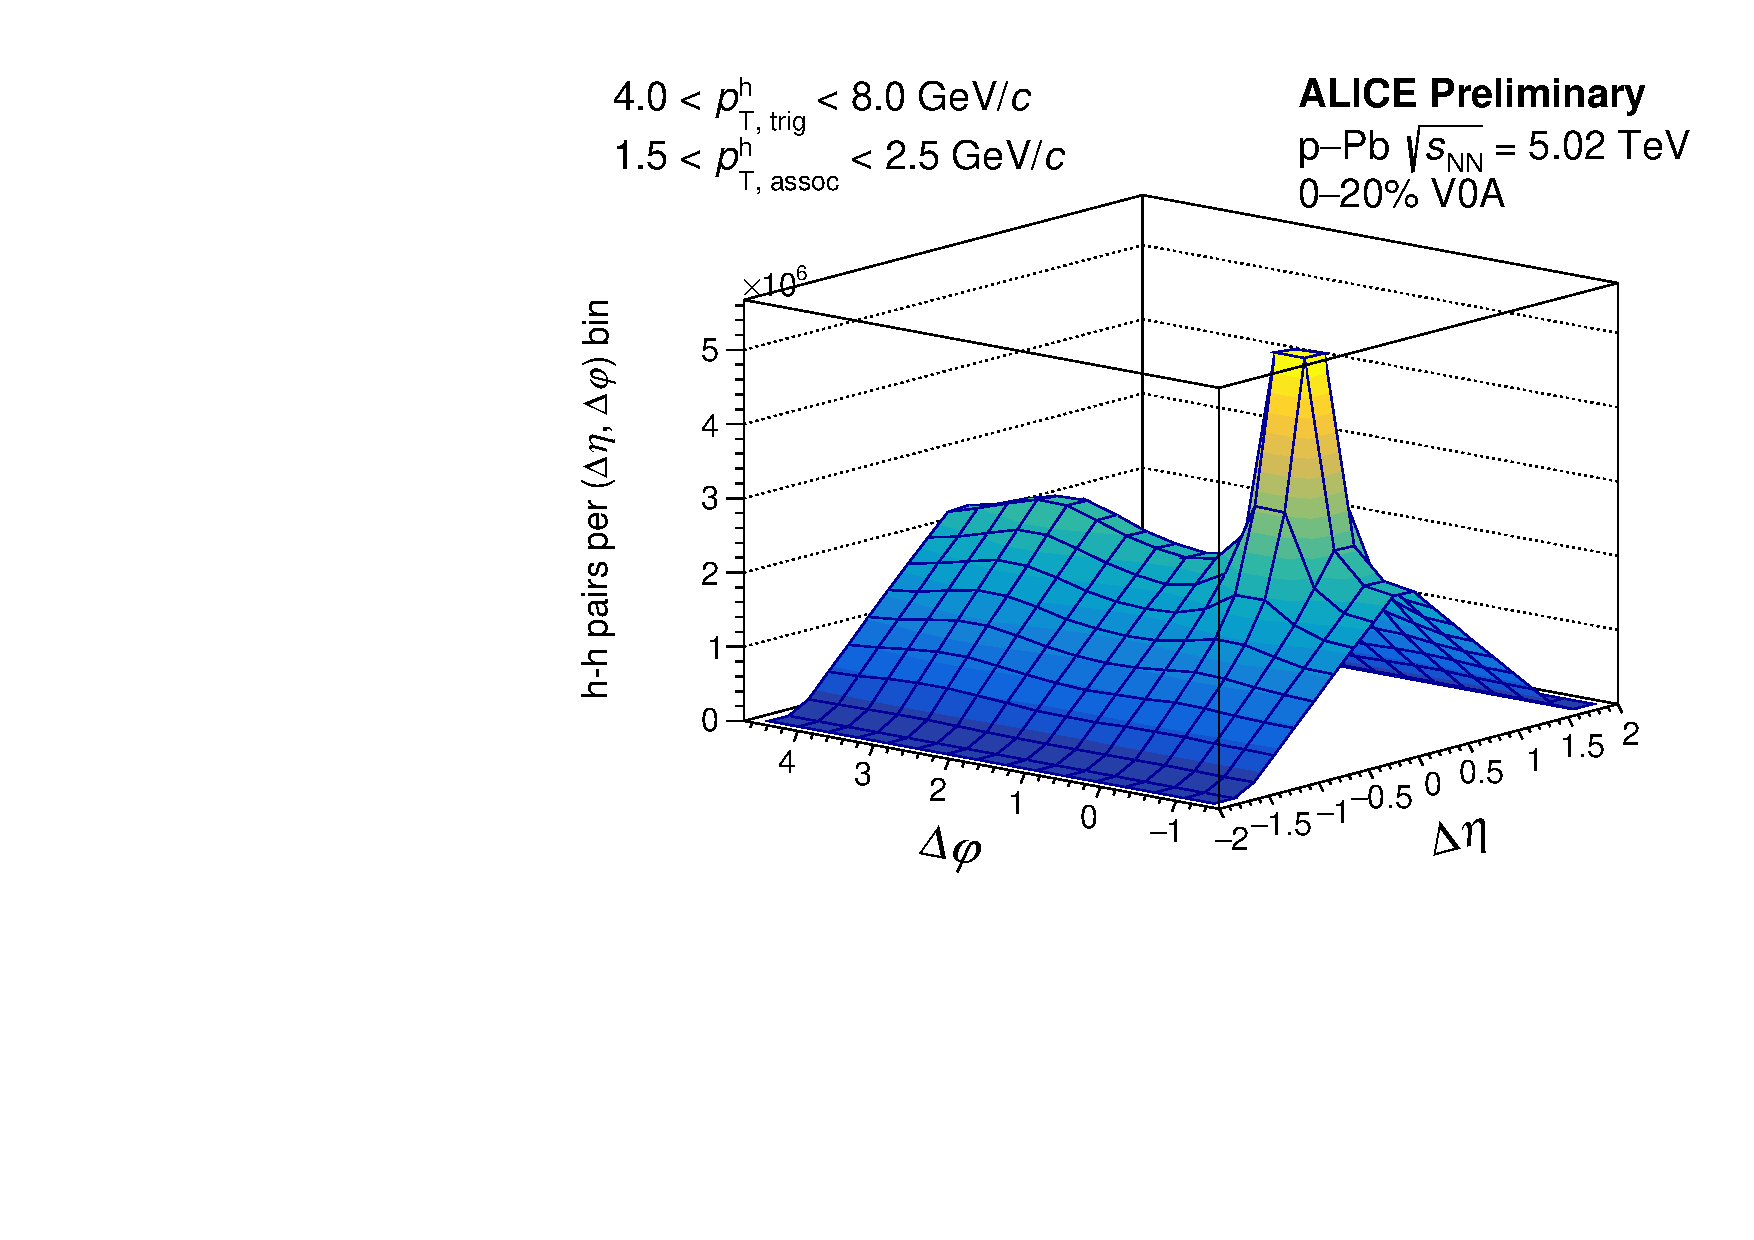
\includegraphics[width=\textwidth]{figures/analysis/h_h_2d_nomixcor_fancy_label_0_20_lowpt.pdf}
	\end{minipage}
	\begin{minipage}{0.48\textwidth}
		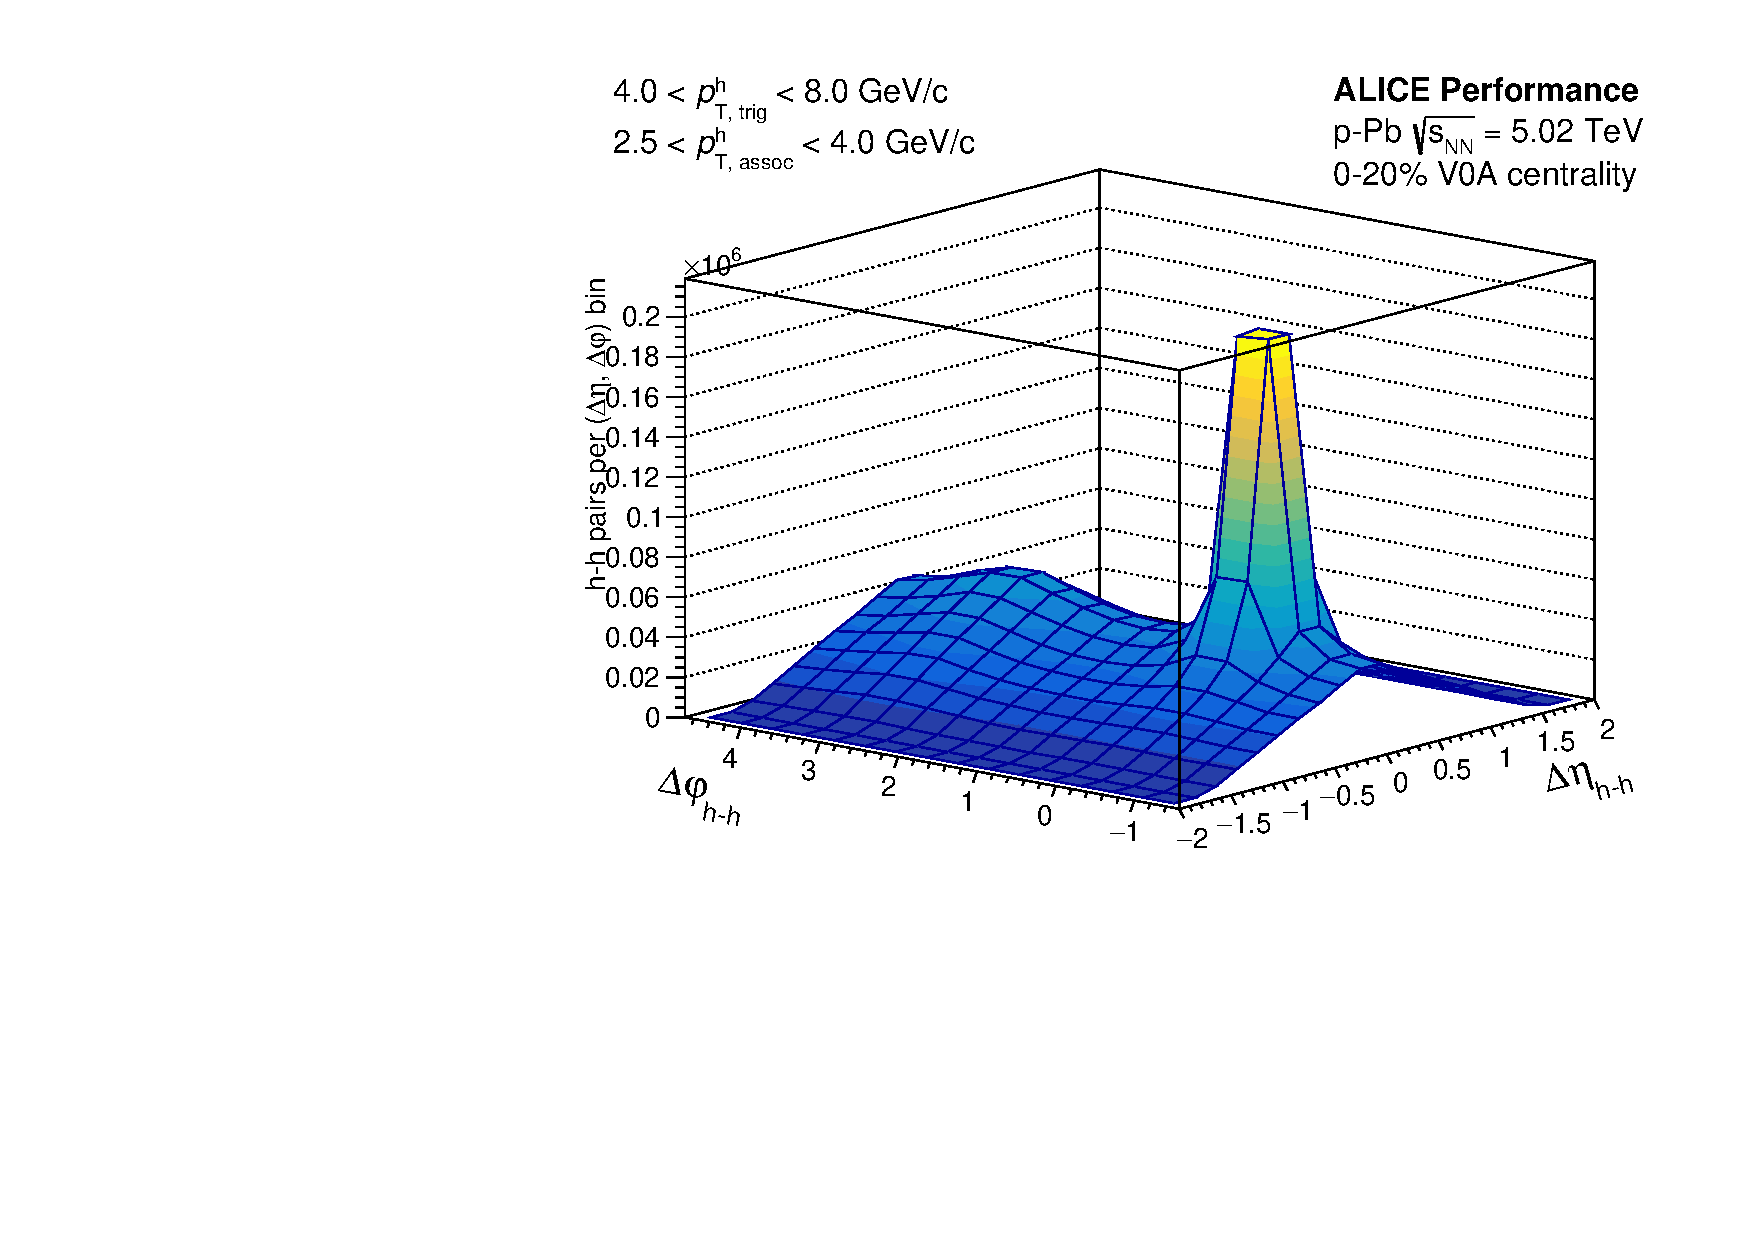
\includegraphics[width=\textwidth]{figures/analysis/h_h_2d_nomixcor_fancy_label_0_20_highpt.pdf}
	\end{minipage}
	\begin{minipage}{0.48\textwidth}
		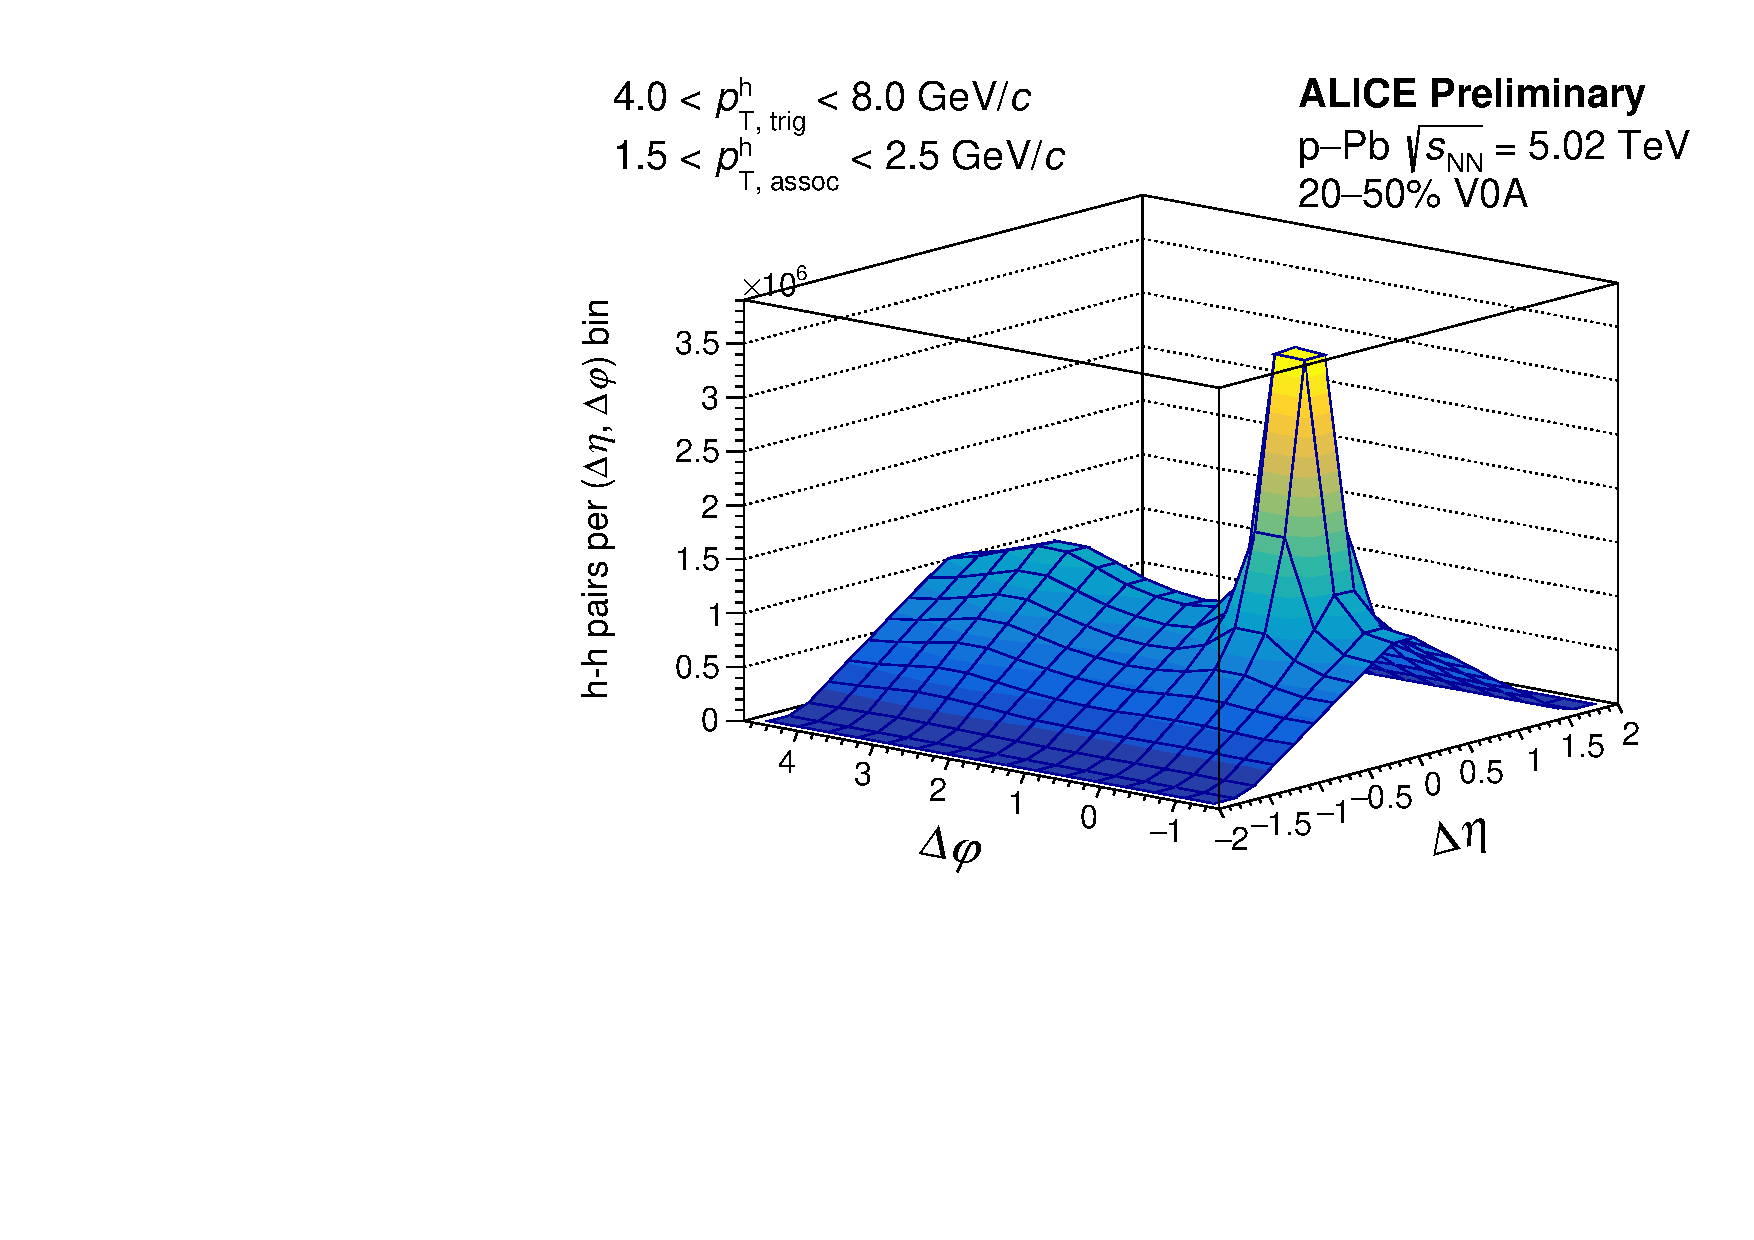
\includegraphics[width=\textwidth]{figures/analysis/h_h_2d_nomixcor_fancy_label_20_50_lowpt.pdf}
	\end{minipage}
	\begin{minipage}{0.48\textwidth}
		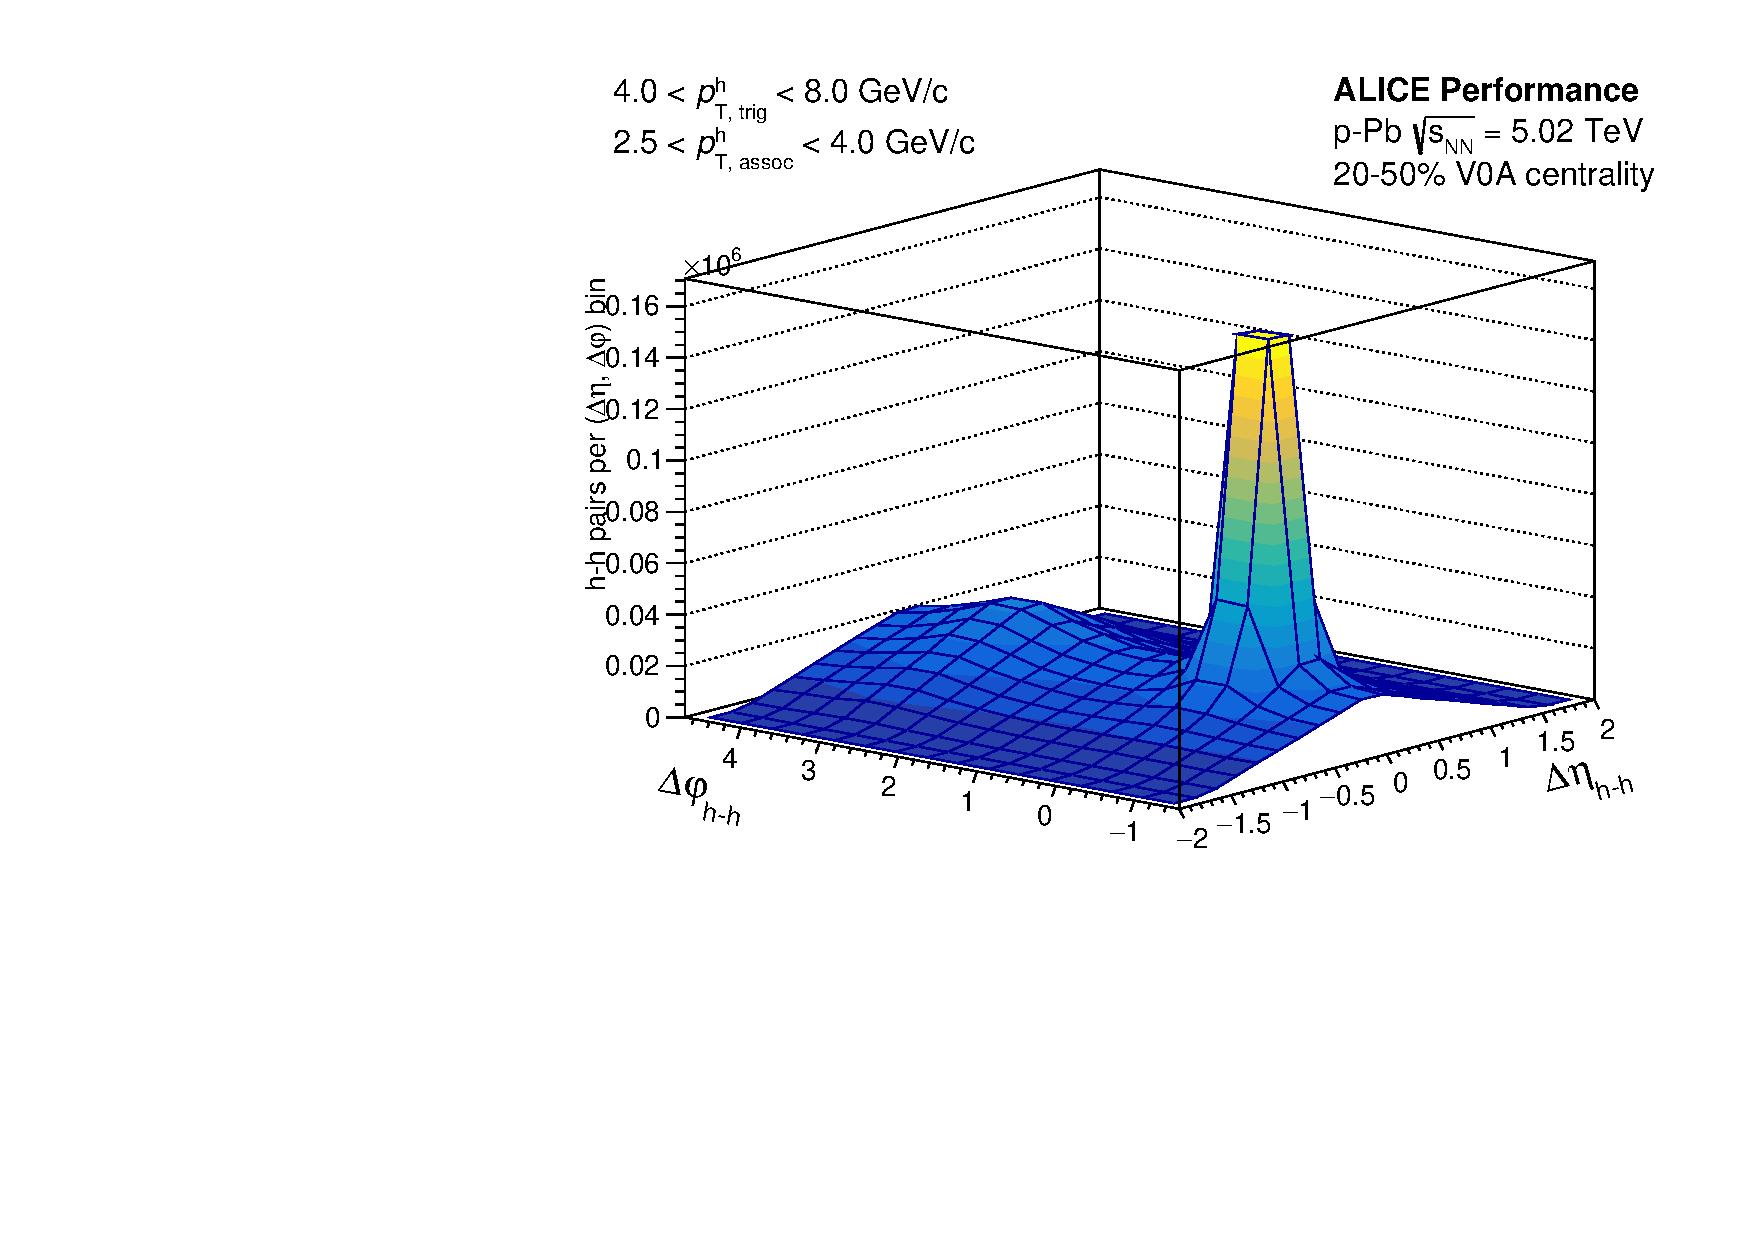
\includegraphics[width=\textwidth]{figures/analysis/h_h_2d_nomixcor_fancy_label_20_50_highpt.pdf}
	\end{minipage}
	\begin{minipage}{0.48\textwidth}
		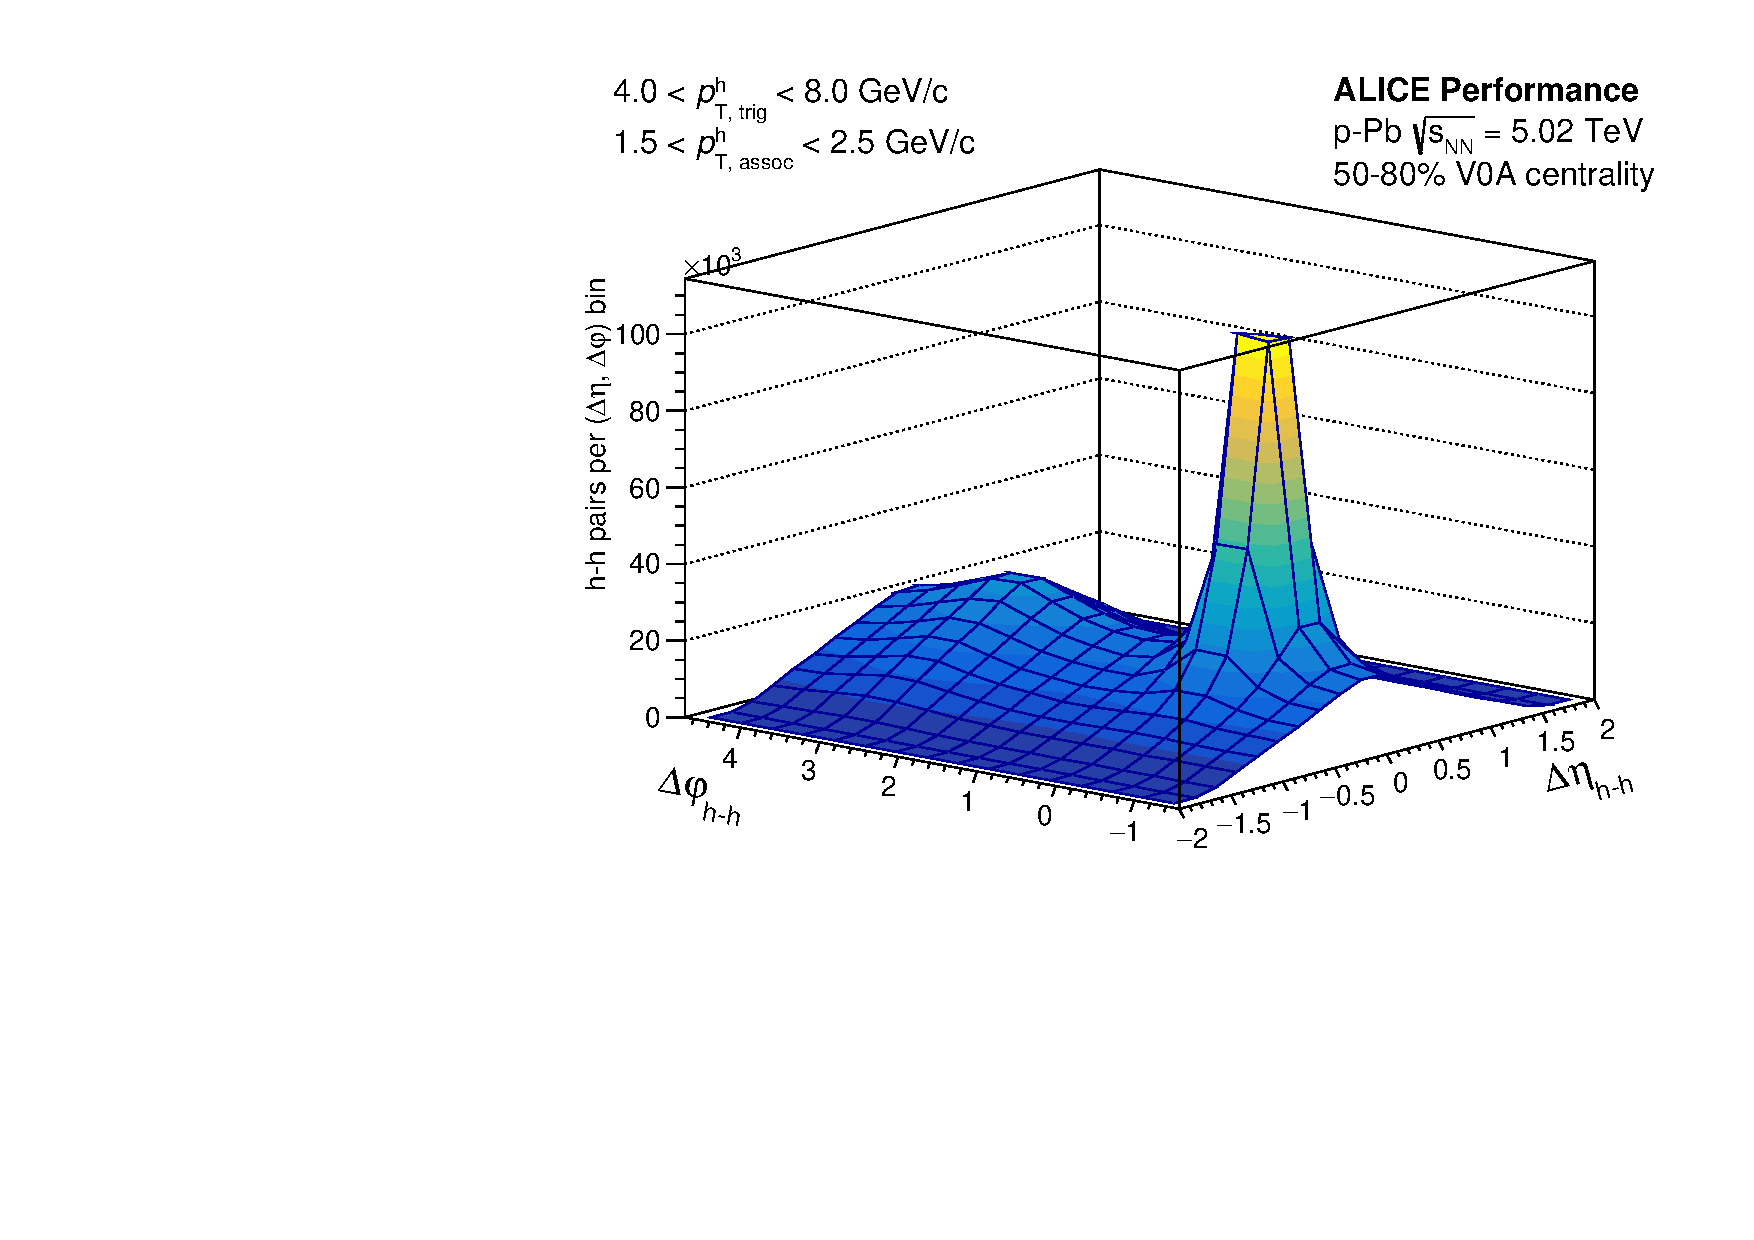
\includegraphics[width=\textwidth]{figures/analysis/h_h_2d_nomixcor_fancy_label_50_80_lowpt.pdf}
	\end{minipage}
	\begin{minipage}{0.48\textwidth}
		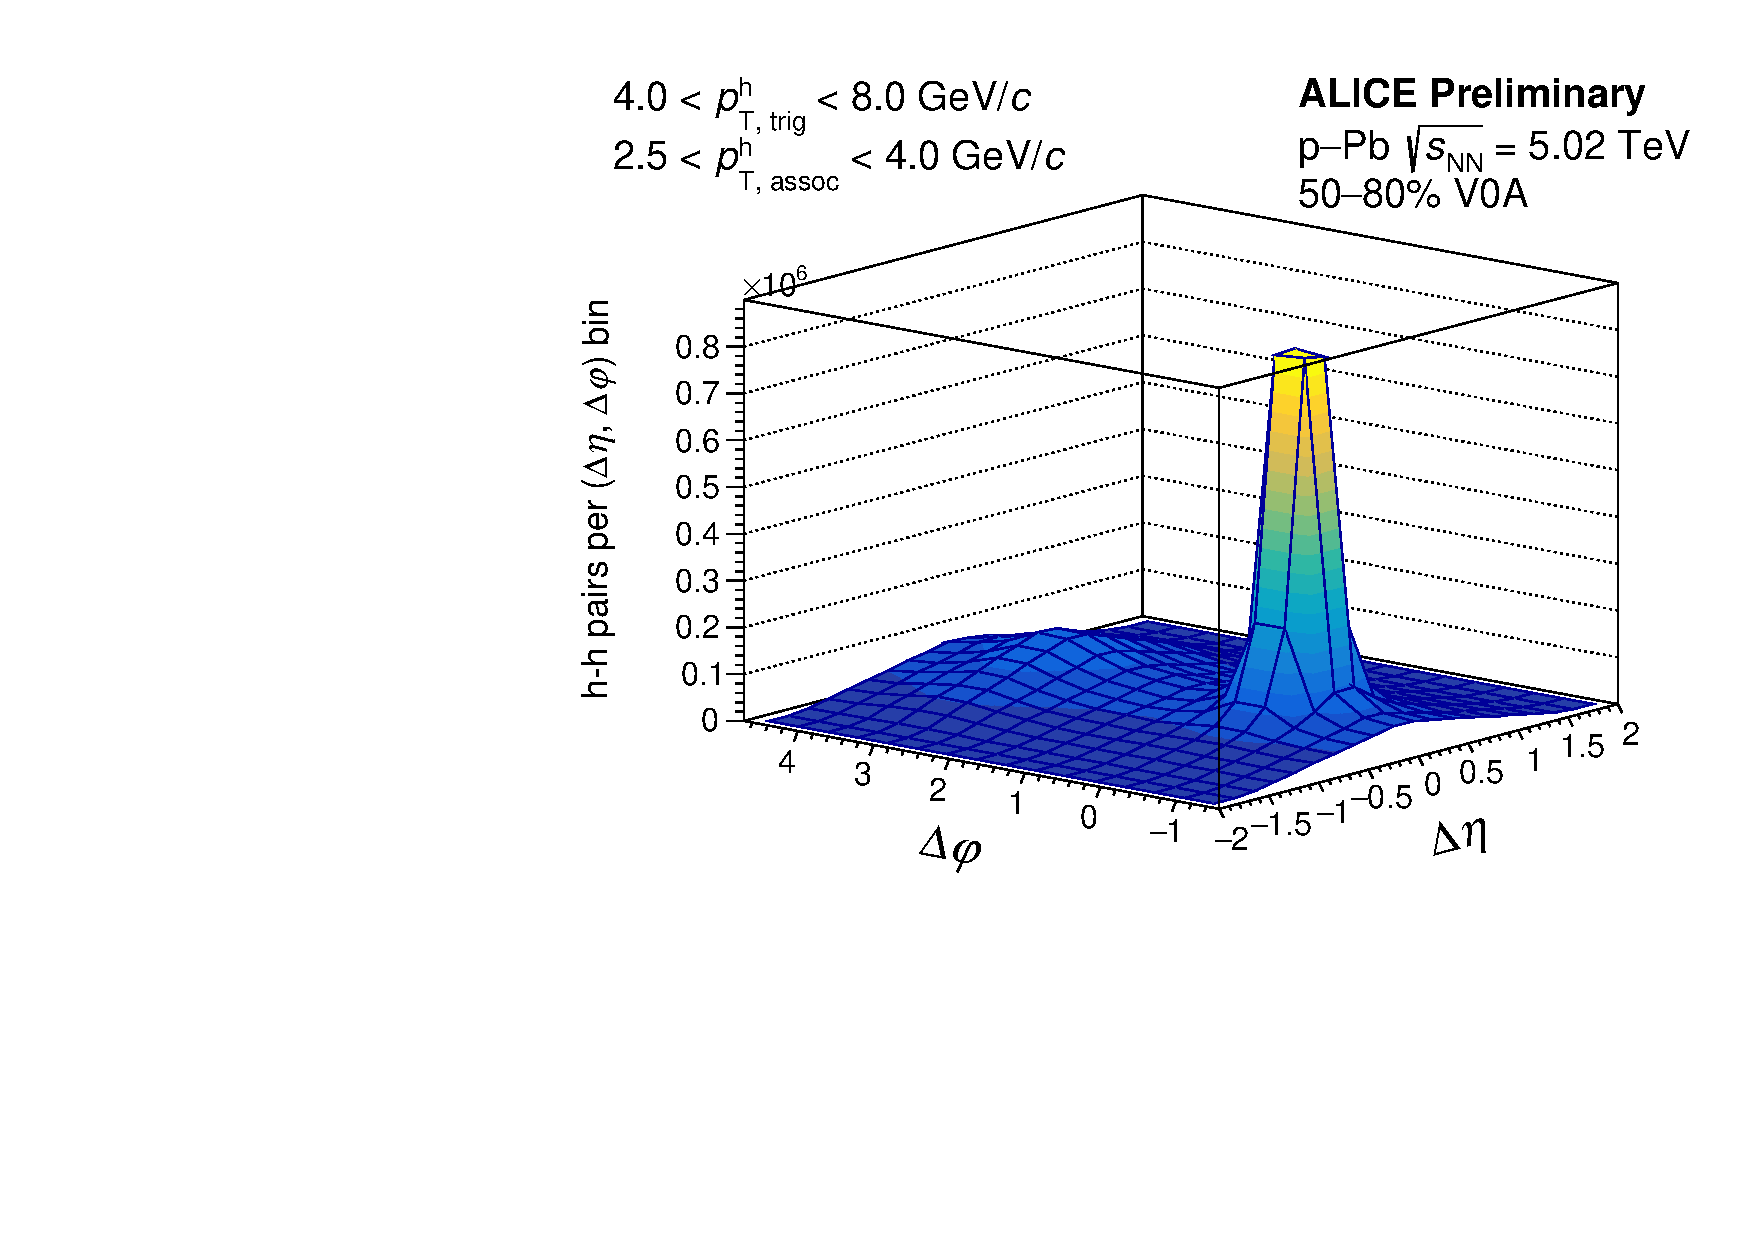
\includegraphics[width=\textwidth]{figures/analysis/h_h_2d_nomixcor_fancy_label_50_80_highpt.pdf}
	\end{minipage}
	\caption{2-D non-acceptance corrected h-h angular correlations for the 0-20\% (top), 20-50\% (middle), and 50-80\% (bottom) multiplicity bins for $1.5 < p_{\text{T}} < 2.5$ GeV/$c$ (left) and $2.5 < p_{\text{T}} < 4.0$ GeV/$c$ (right). The $Z_{\text{vtx.}}$ bins are merged together for these plots.}
	\label{fig:h_h_2d_nomixcor}
\end{figure}

\begin{figure}[ht]
	\centering
	\begin{minipage}{0.48\textwidth}
		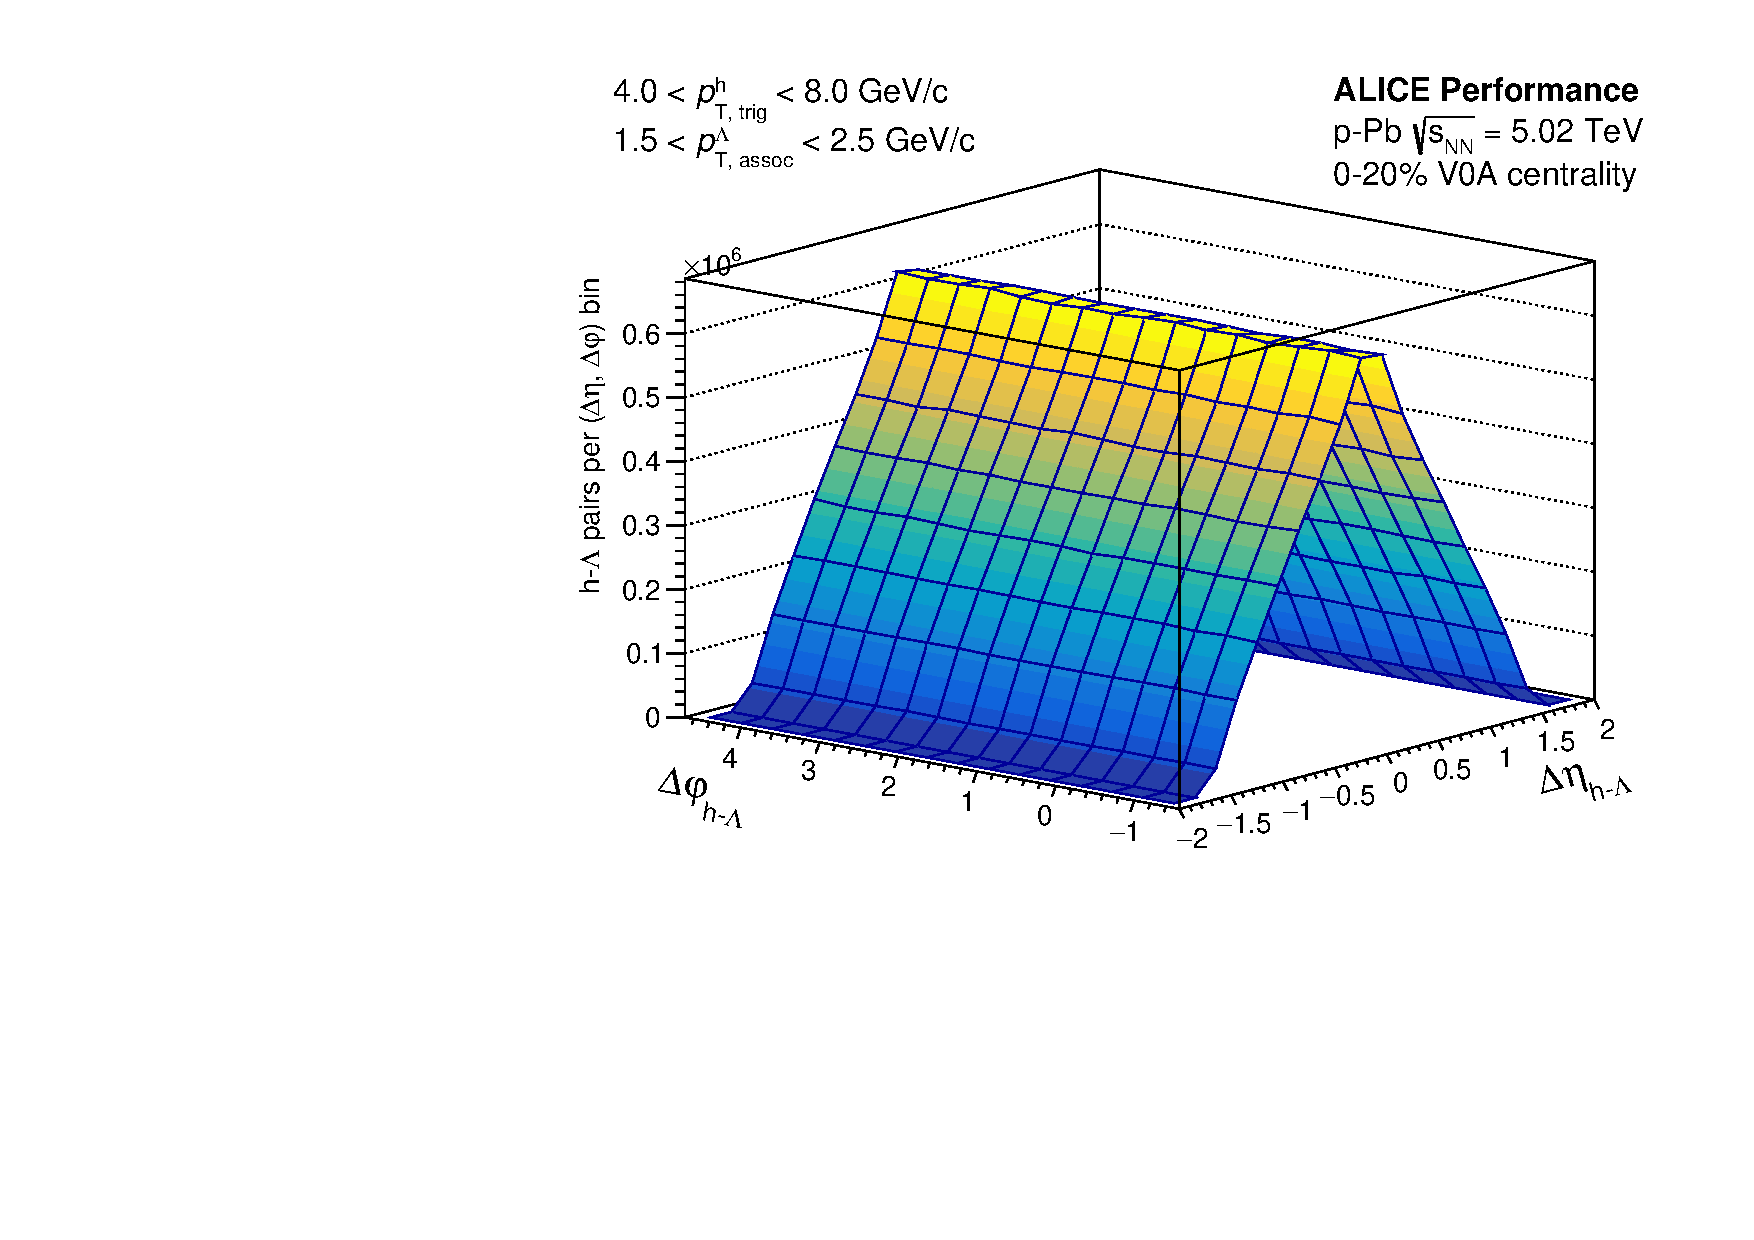
\includegraphics[width=\textwidth]{figures/analysis/h_lambda_2d_mixed_fancy_label_0_20_lowpt.pdf}
	\end{minipage}
	\begin{minipage}{0.48\textwidth}
		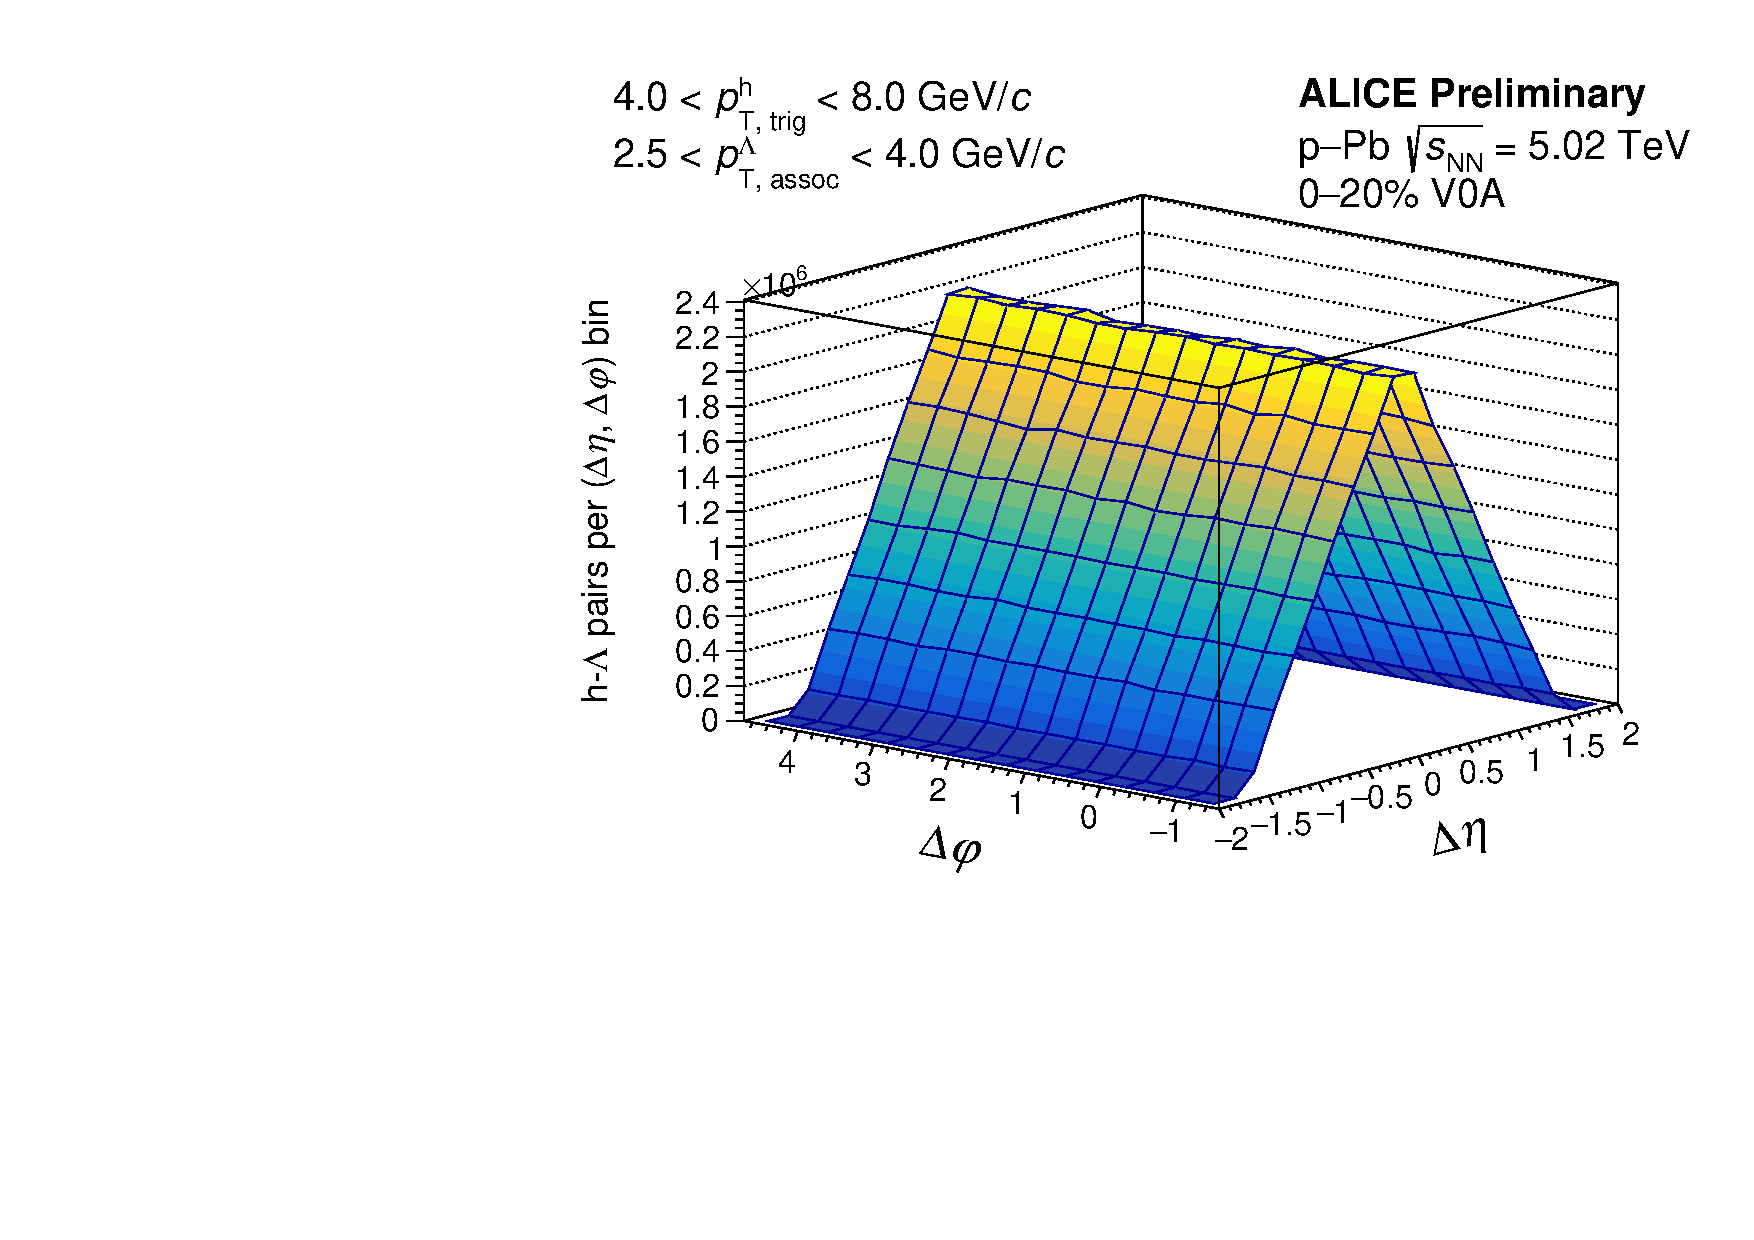
\includegraphics[width=\textwidth]{figures/analysis/h_lambda_2d_mixed_fancy_label_0_20_highpt.pdf}
	\end{minipage}
	\begin{minipage}{0.48\textwidth}
		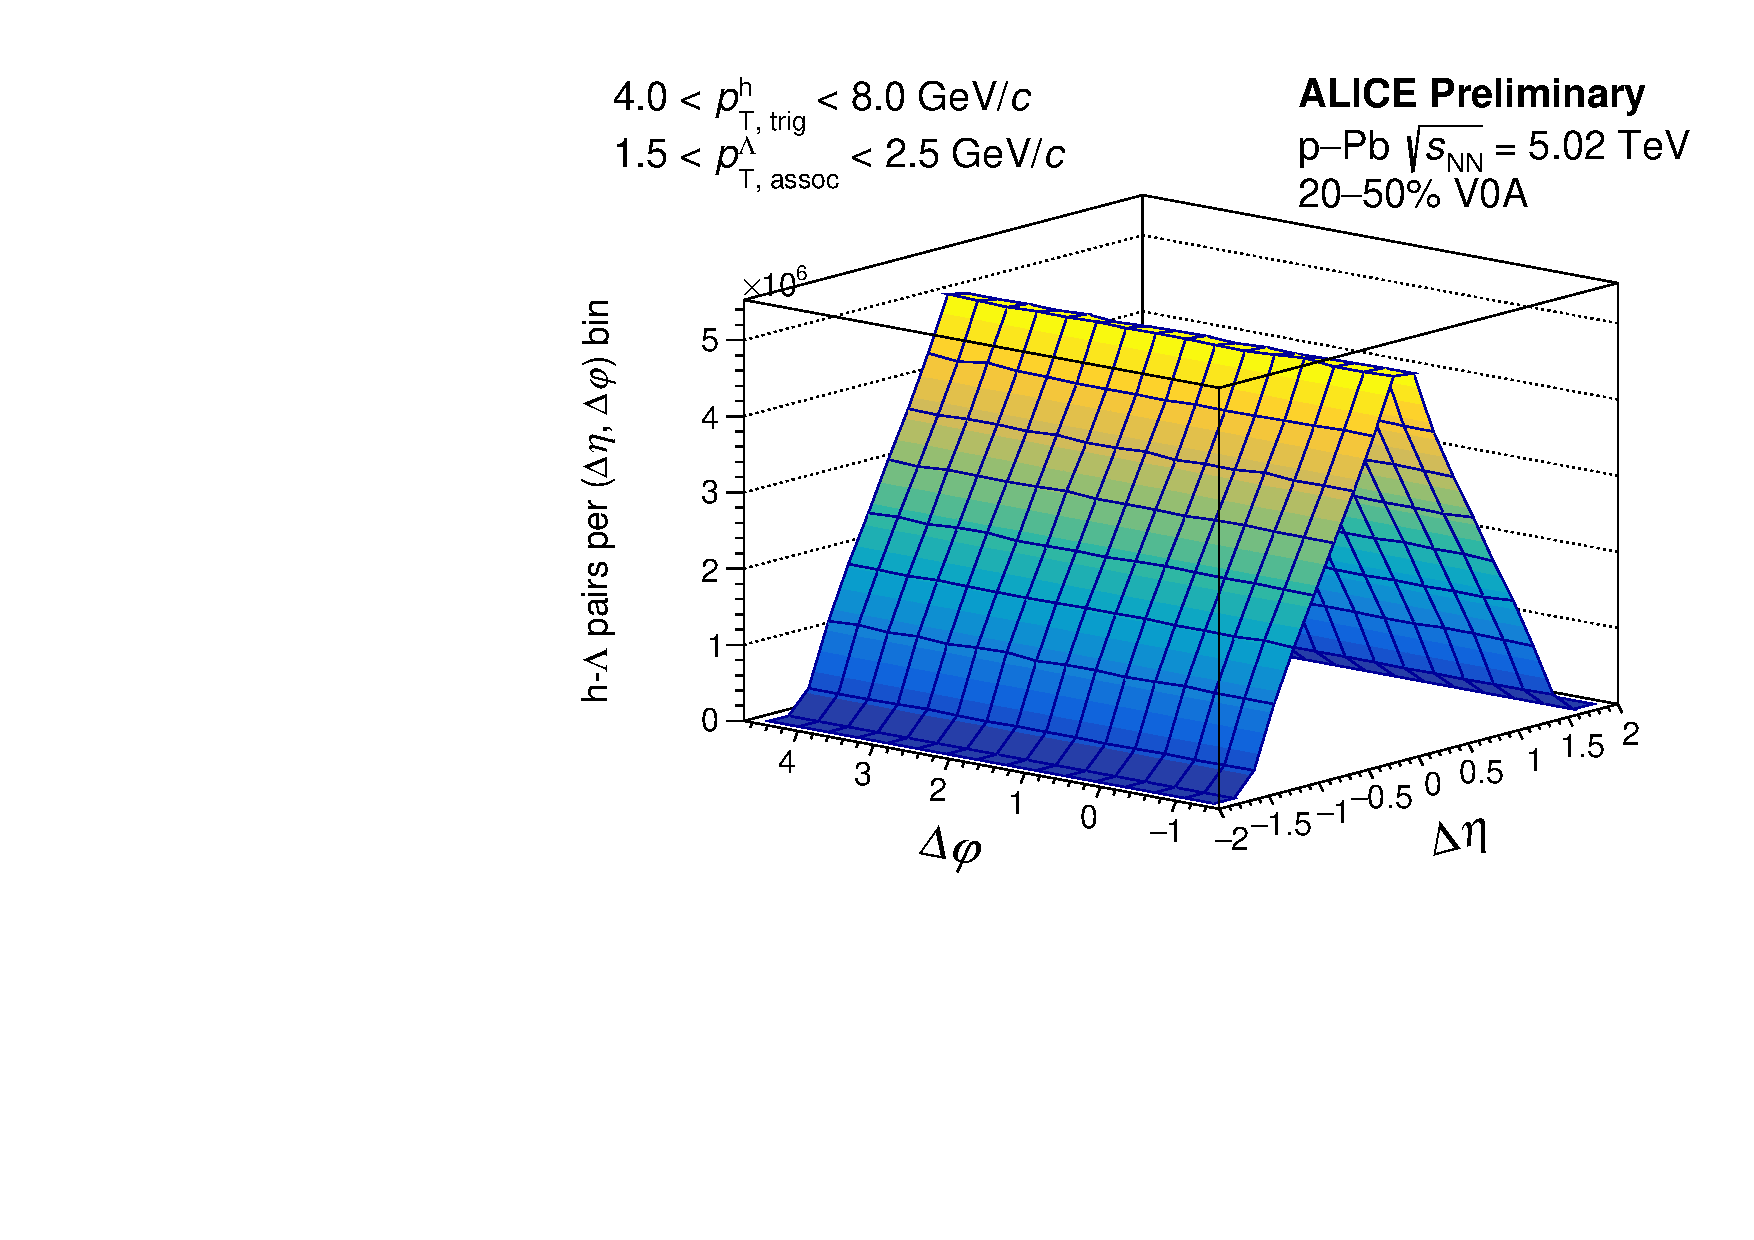
\includegraphics[width=\textwidth]{figures/analysis/h_lambda_2d_mixed_fancy_label_20_50_lowpt.pdf}
	\end{minipage}
	\begin{minipage}{0.48\textwidth}
		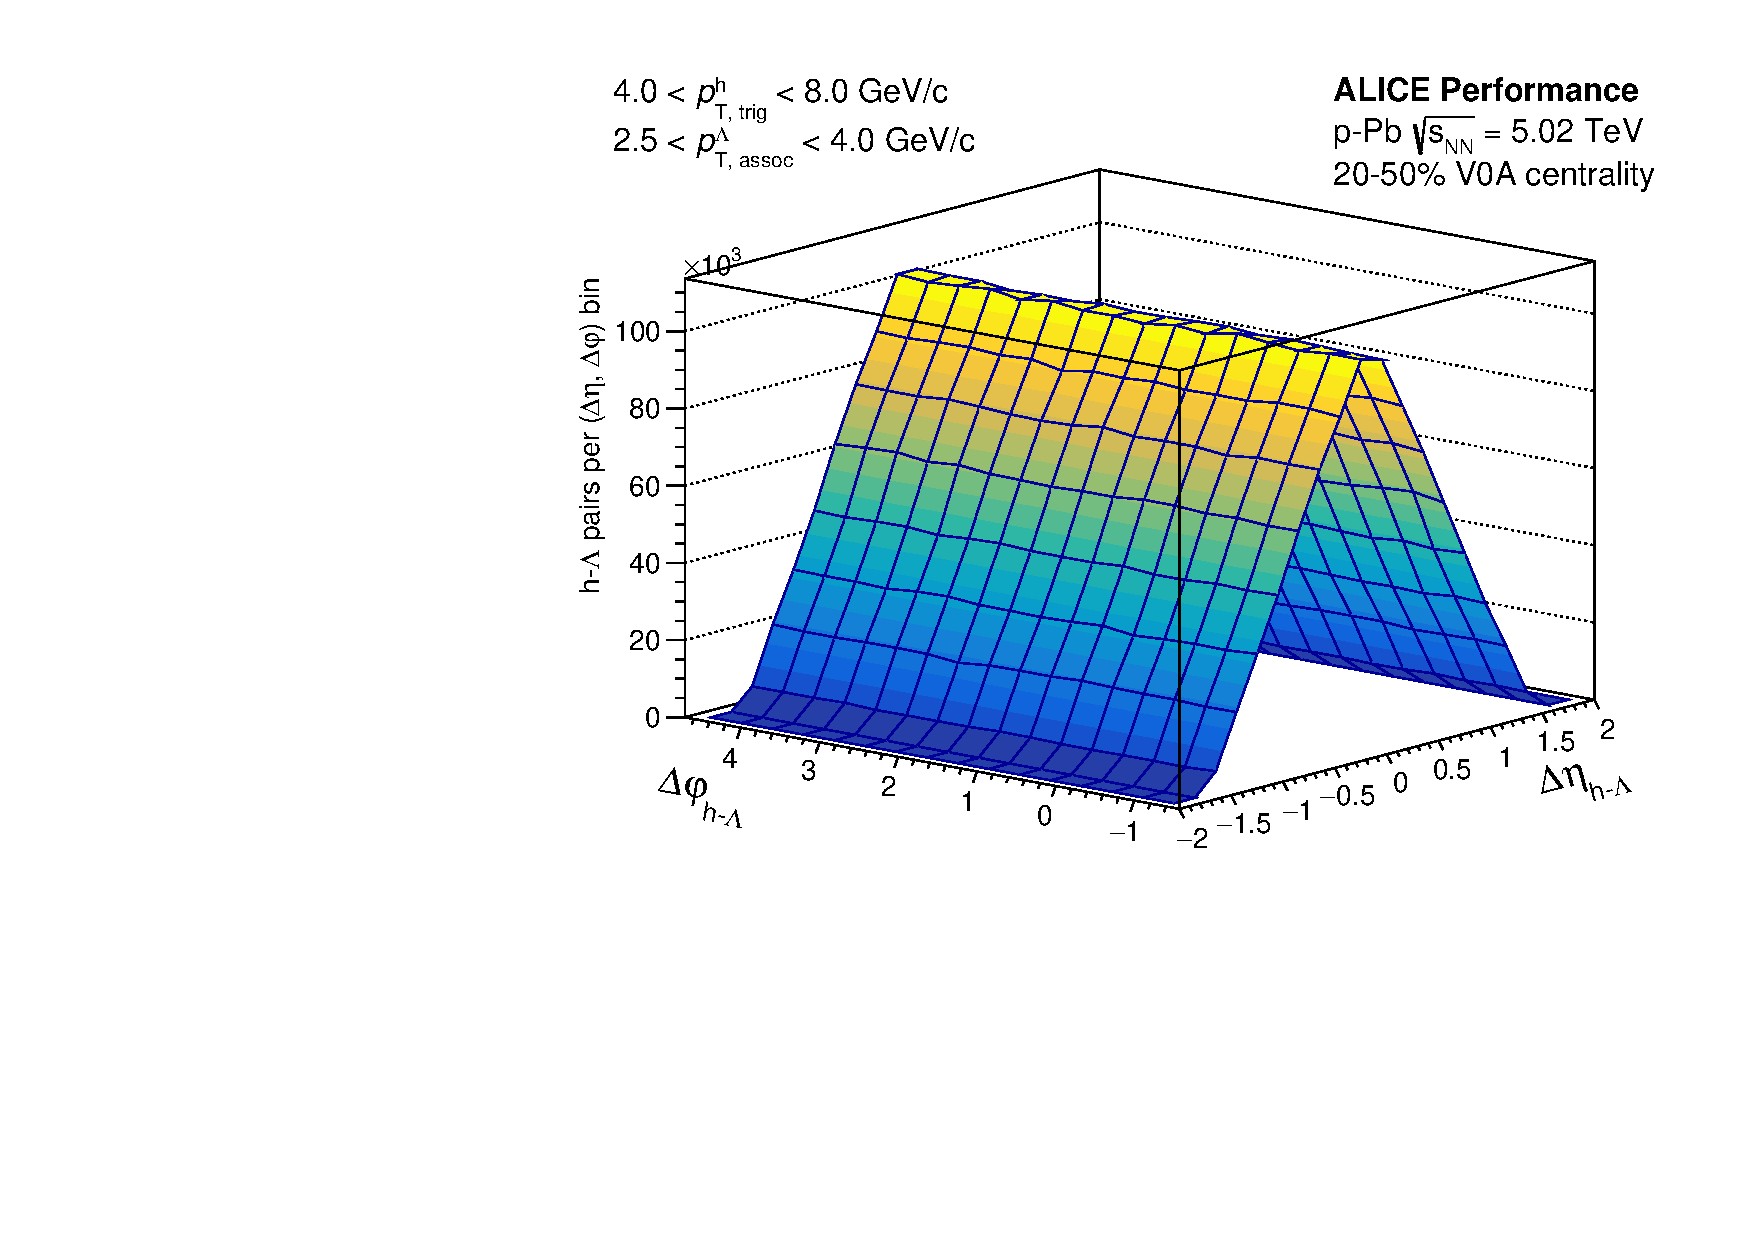
\includegraphics[width=\textwidth]{figures/analysis/h_lambda_2d_mixed_fancy_label_20_50_highpt.pdf}
	\end{minipage}
	\begin{minipage}{0.48\textwidth}
		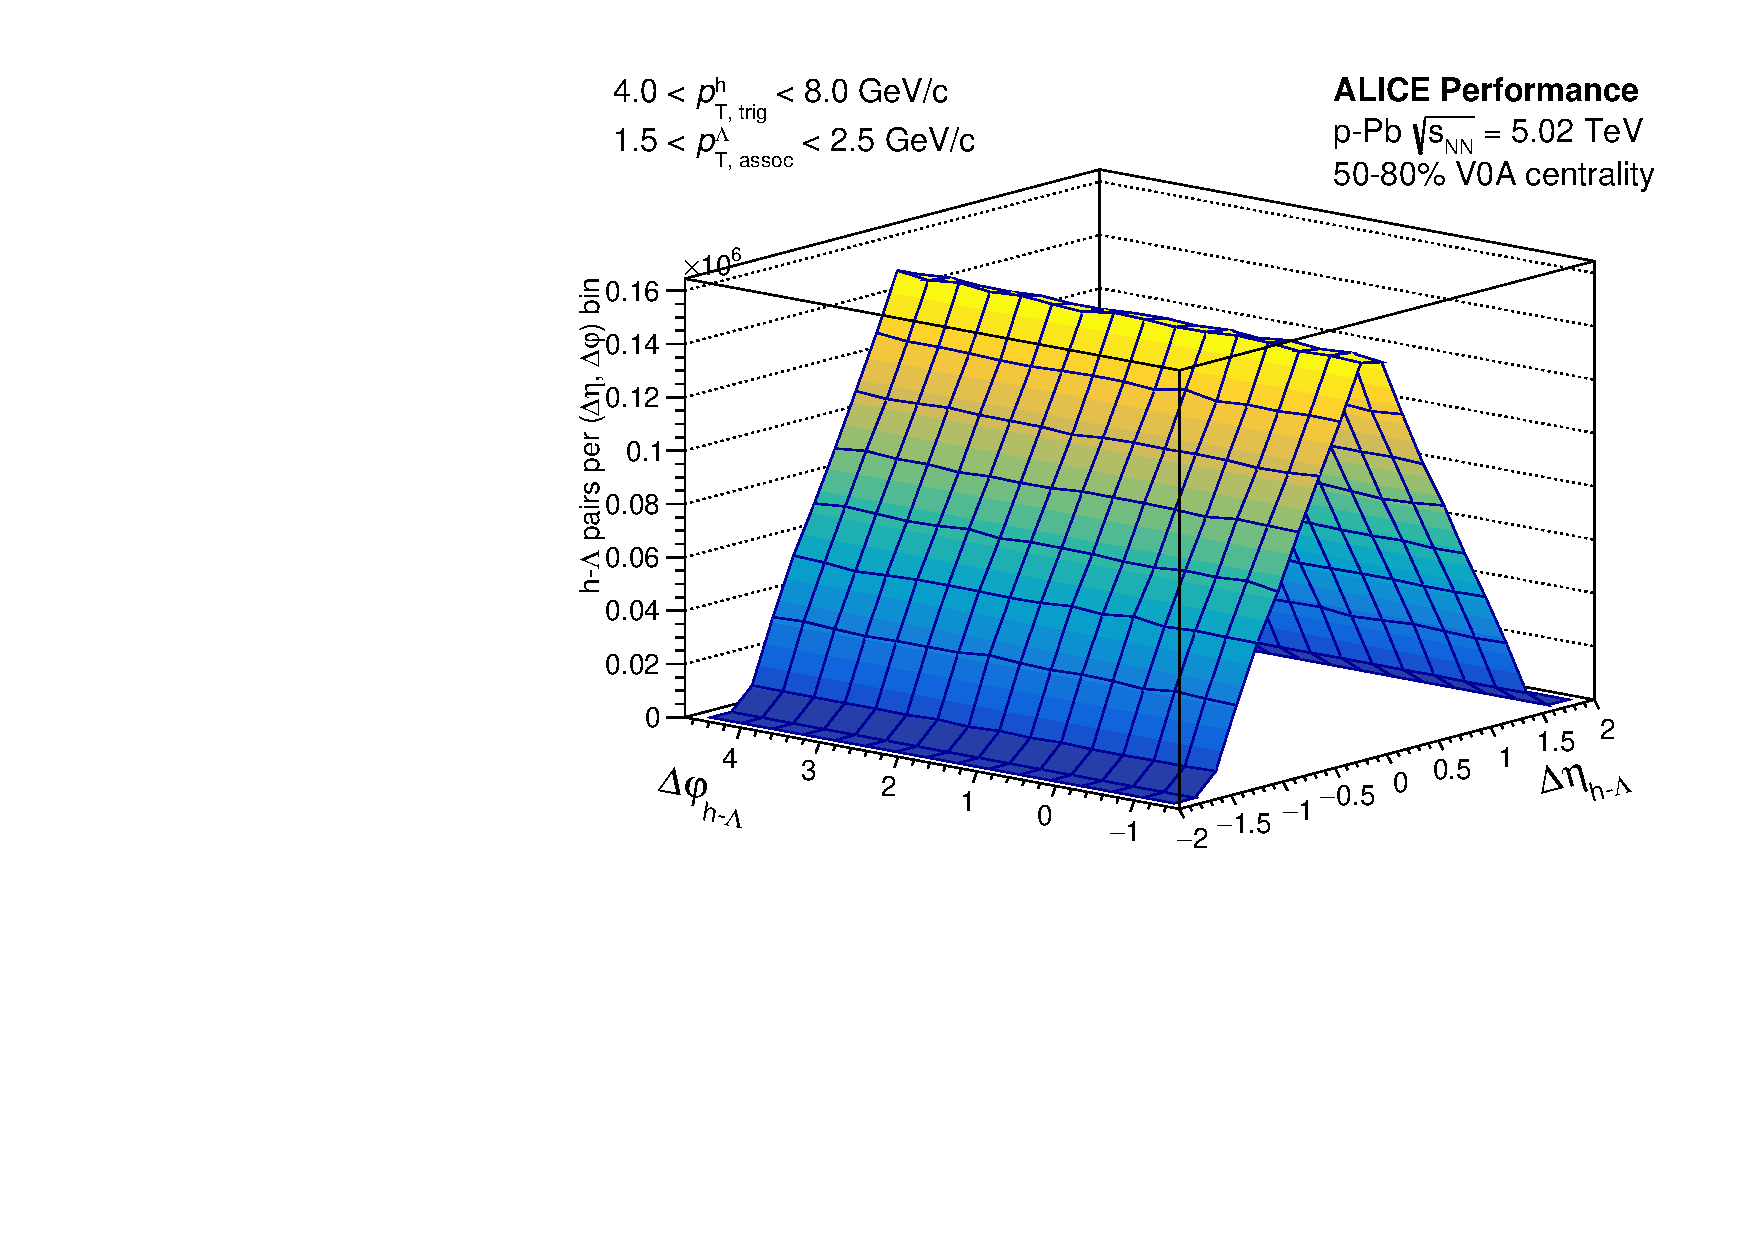
\includegraphics[width=\textwidth]{figures/analysis/h_lambda_2d_mixed_fancy_label_50_80_lowpt.pdf}
	\end{minipage}
	\begin{minipage}{0.48\textwidth}
		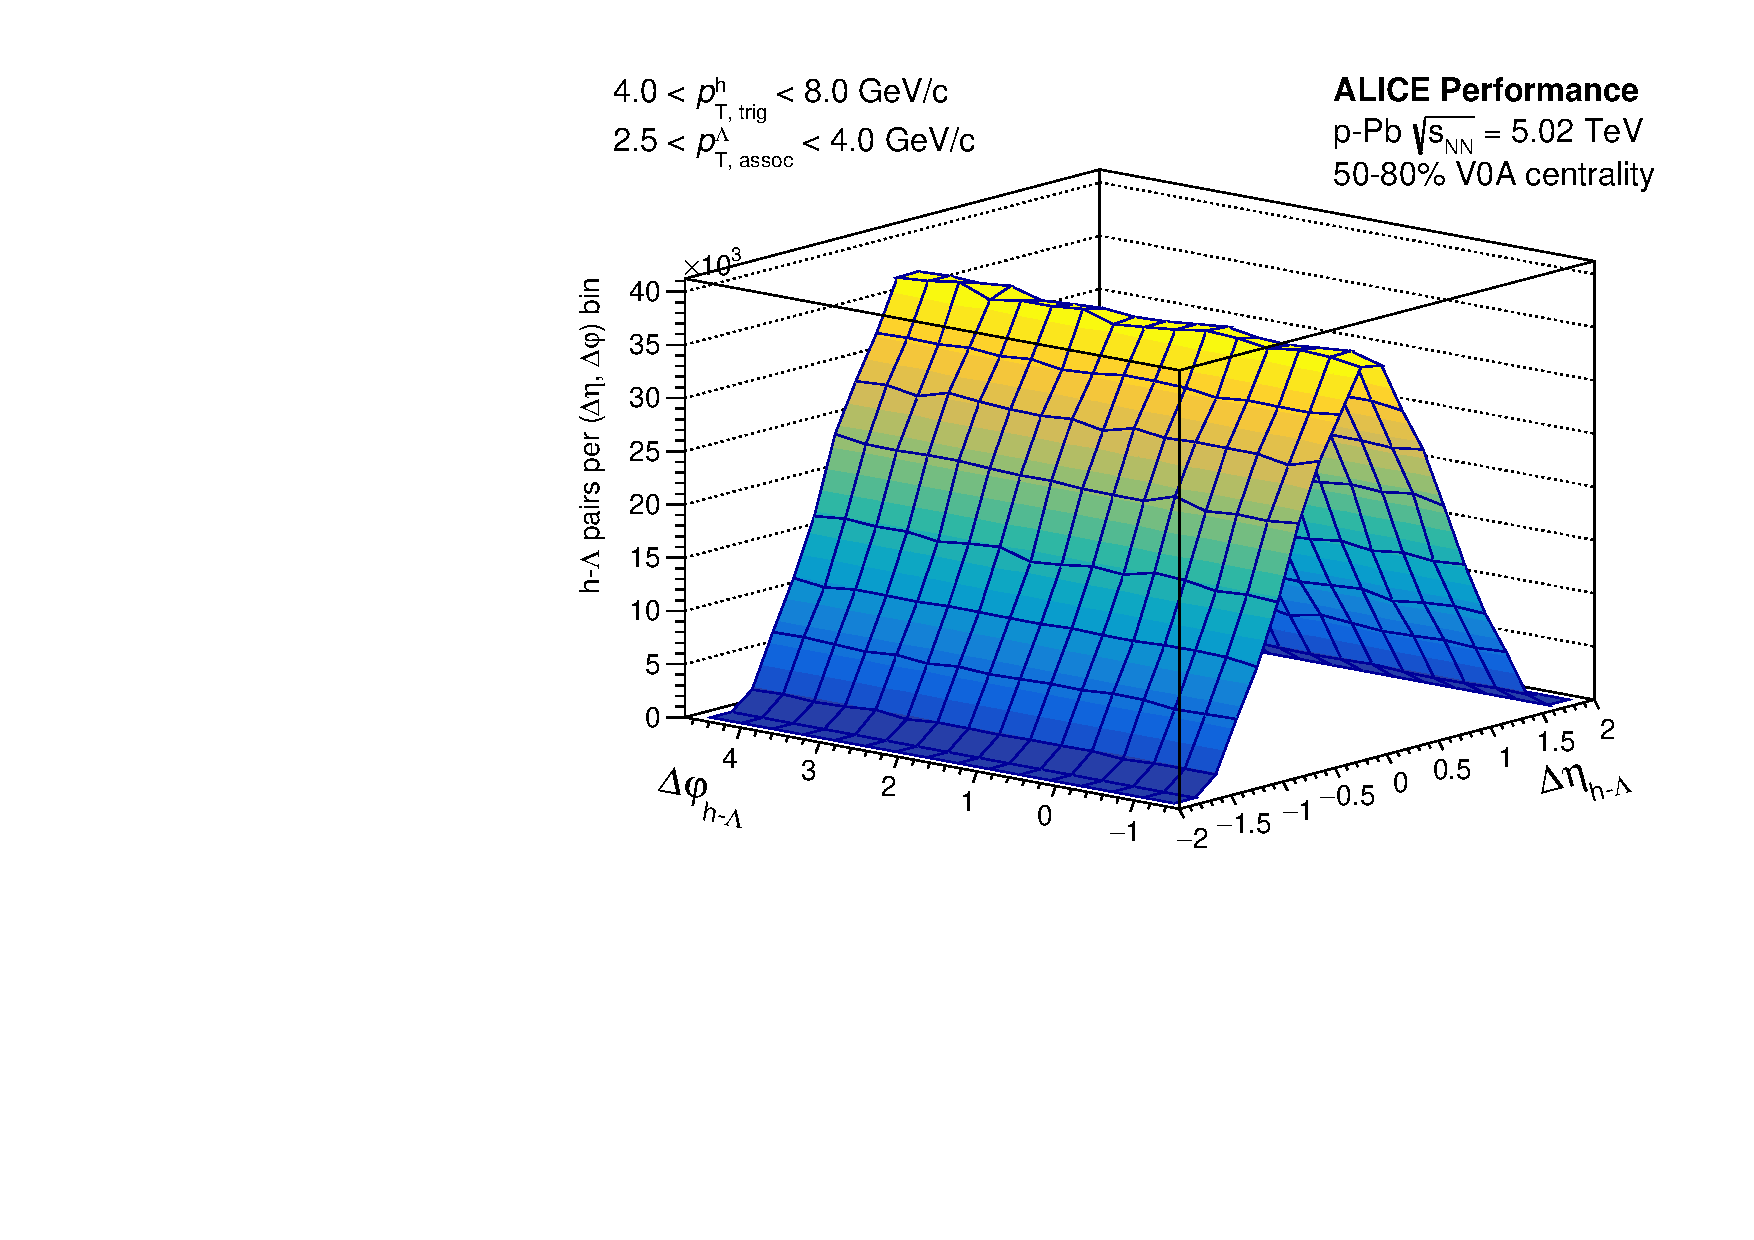
\includegraphics[width=\textwidth]{figures/analysis/h_lambda_2d_mixed_fancy_label_50_80_highpt.pdf}
	\end{minipage}
	\caption{2-D mixed-event h-$\Lambda$ angular correlations for the 0-20\% (top), 20-50\% (middle), and 50-80\% (bottom) multiplicity bins for $1.5 < p_{\text{T}} < 2.5$ GeV/$c$ (left) and $2.5 < p_{\text{T}} < 4.0$ GeV/$c$ (right). The $Z_{\text{vtx.}}$ bins are merged together for these plots.}
	\label{fig:h_lambda_2d_mixed}
\end{figure}
\begin{figure}[ht]
	\centering
	\begin{minipage}{0.48\textwidth}
		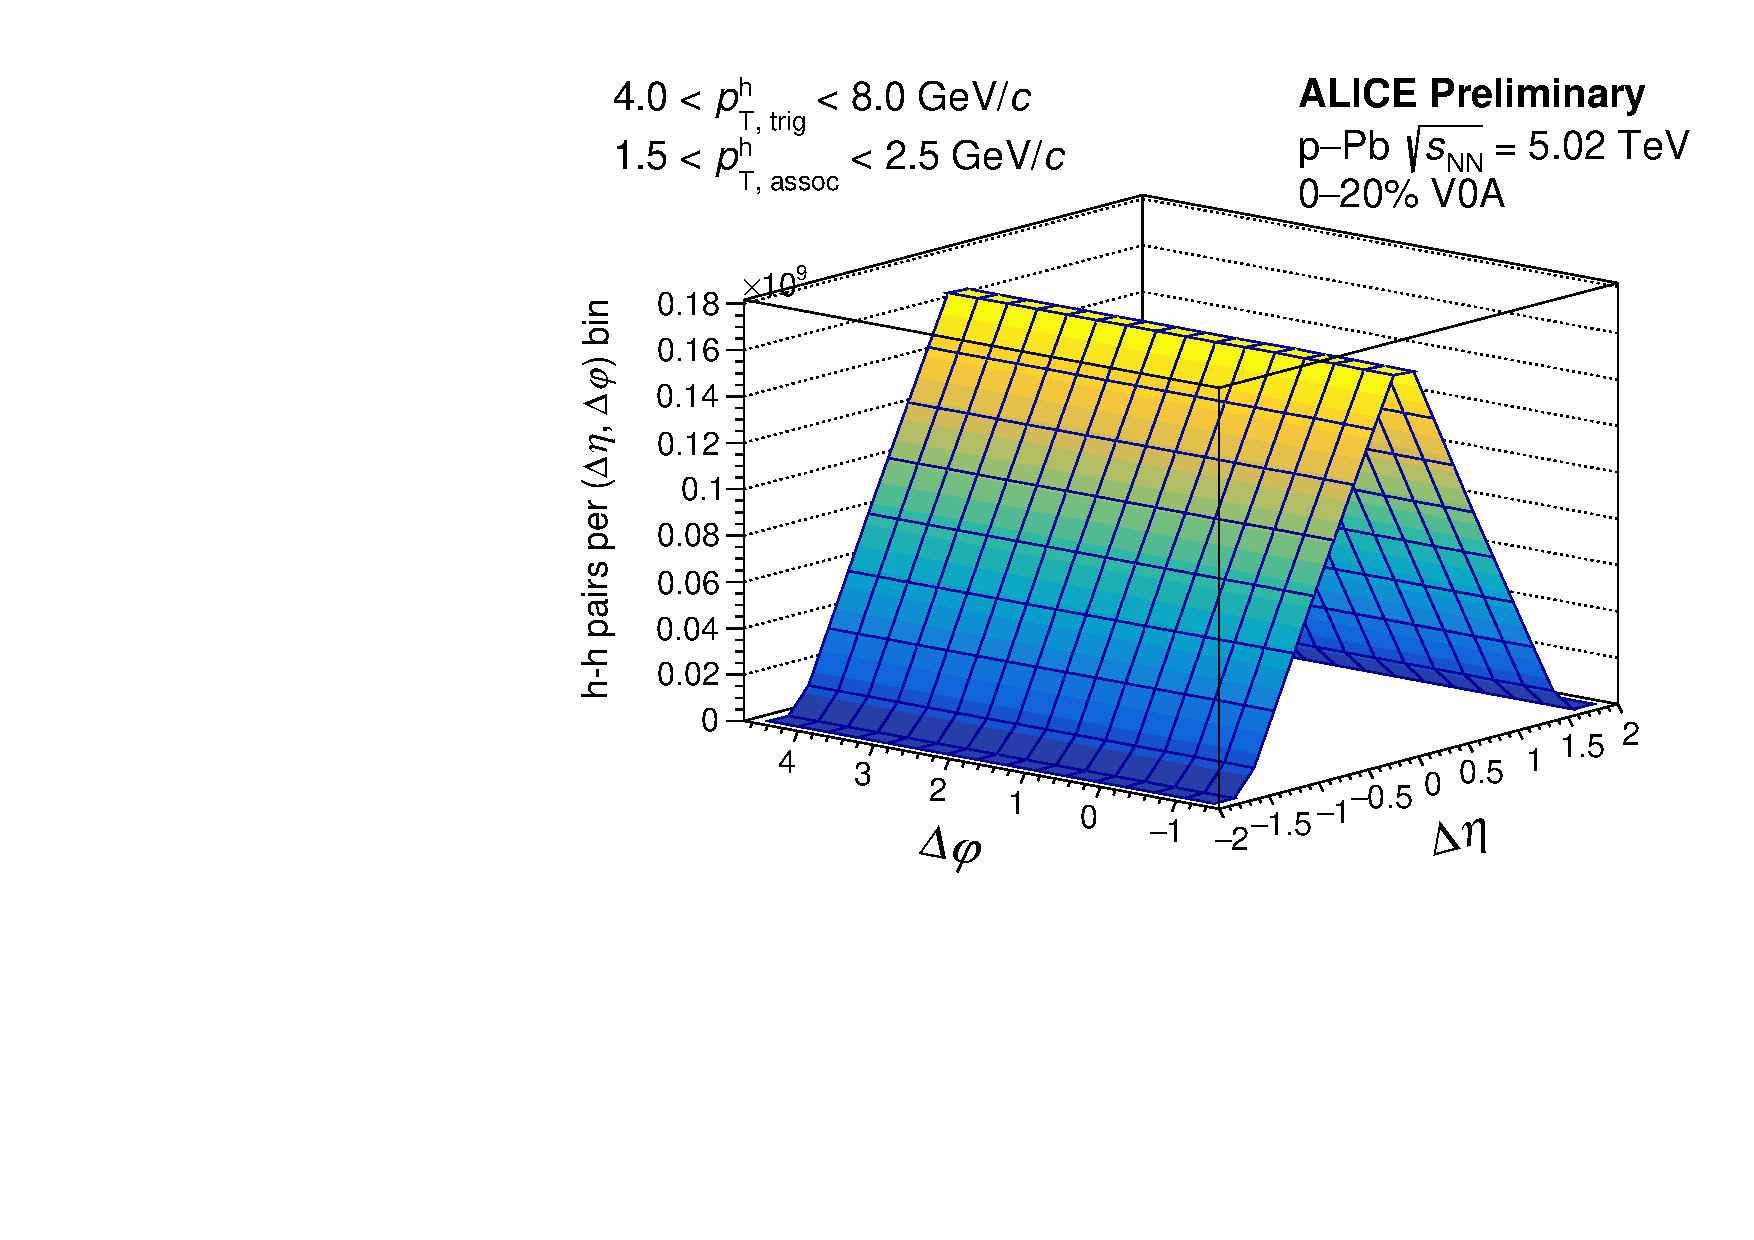
\includegraphics[width=\textwidth]{figures/analysis/h_h_2d_mixed_fancy_label_0_20_lowpt.pdf}
	\end{minipage}
	\begin{minipage}{0.48\textwidth}
		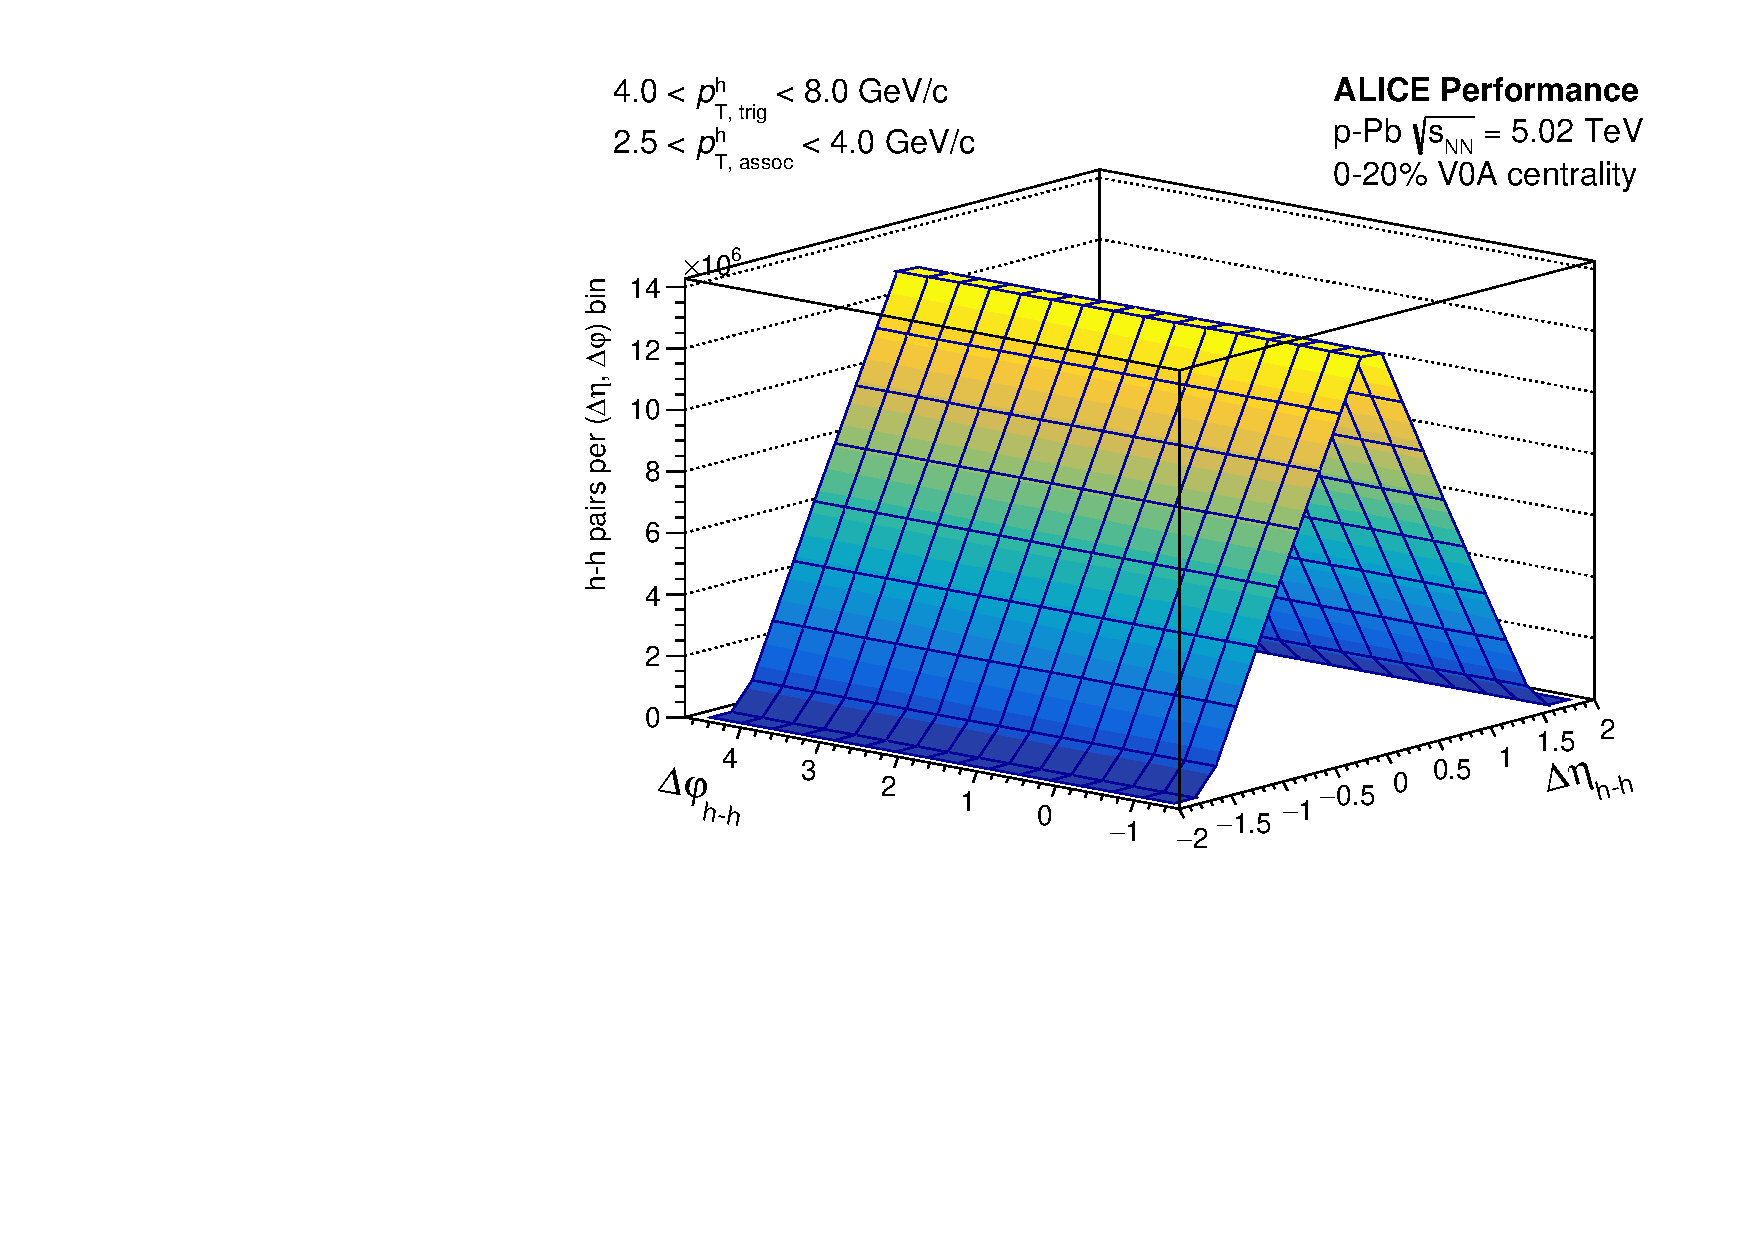
\includegraphics[width=\textwidth]{figures/analysis/h_h_2d_mixed_fancy_label_0_20_highpt.pdf}
	\end{minipage}
	\begin{minipage}{0.48\textwidth}
		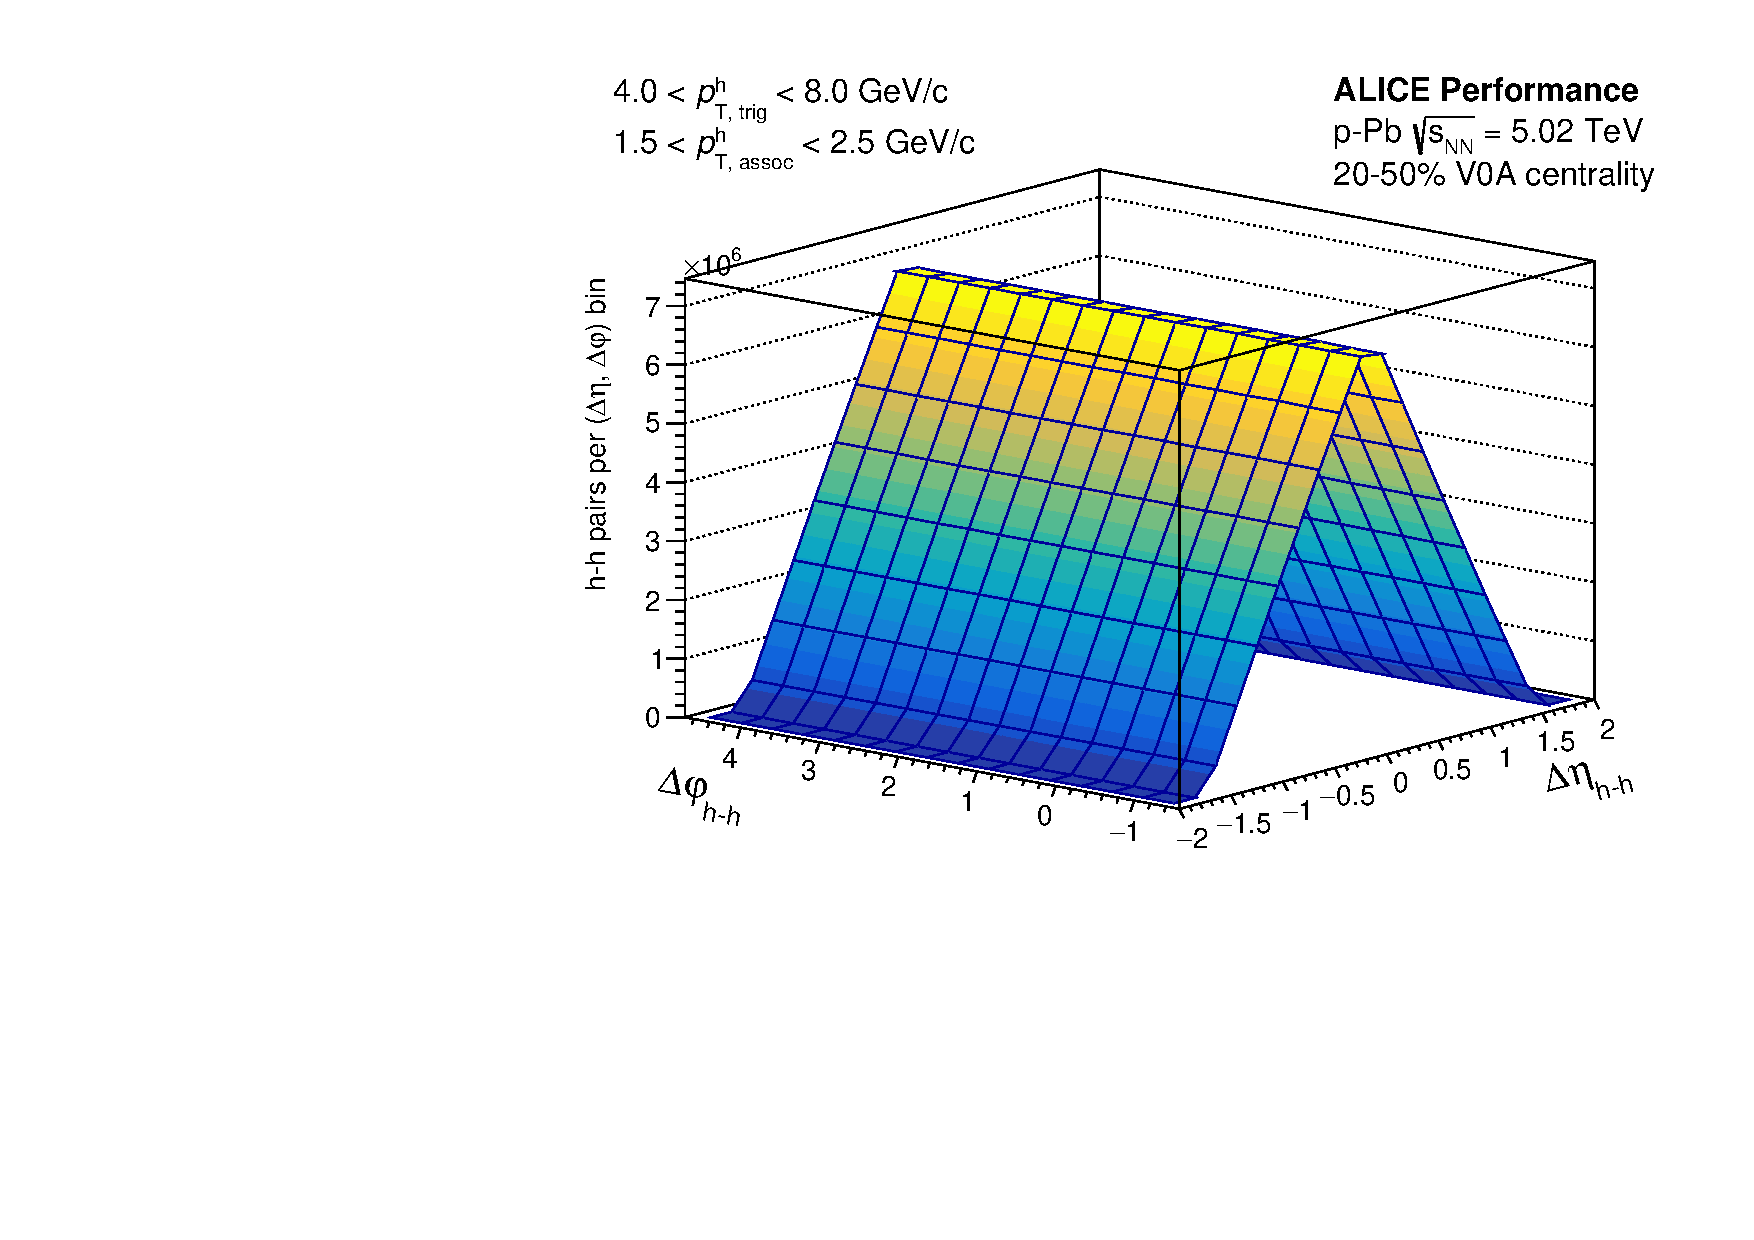
\includegraphics[width=\textwidth]{figures/analysis/h_h_2d_mixed_fancy_label_20_50_lowpt.pdf}
	\end{minipage}
	\begin{minipage}{0.48\textwidth}
		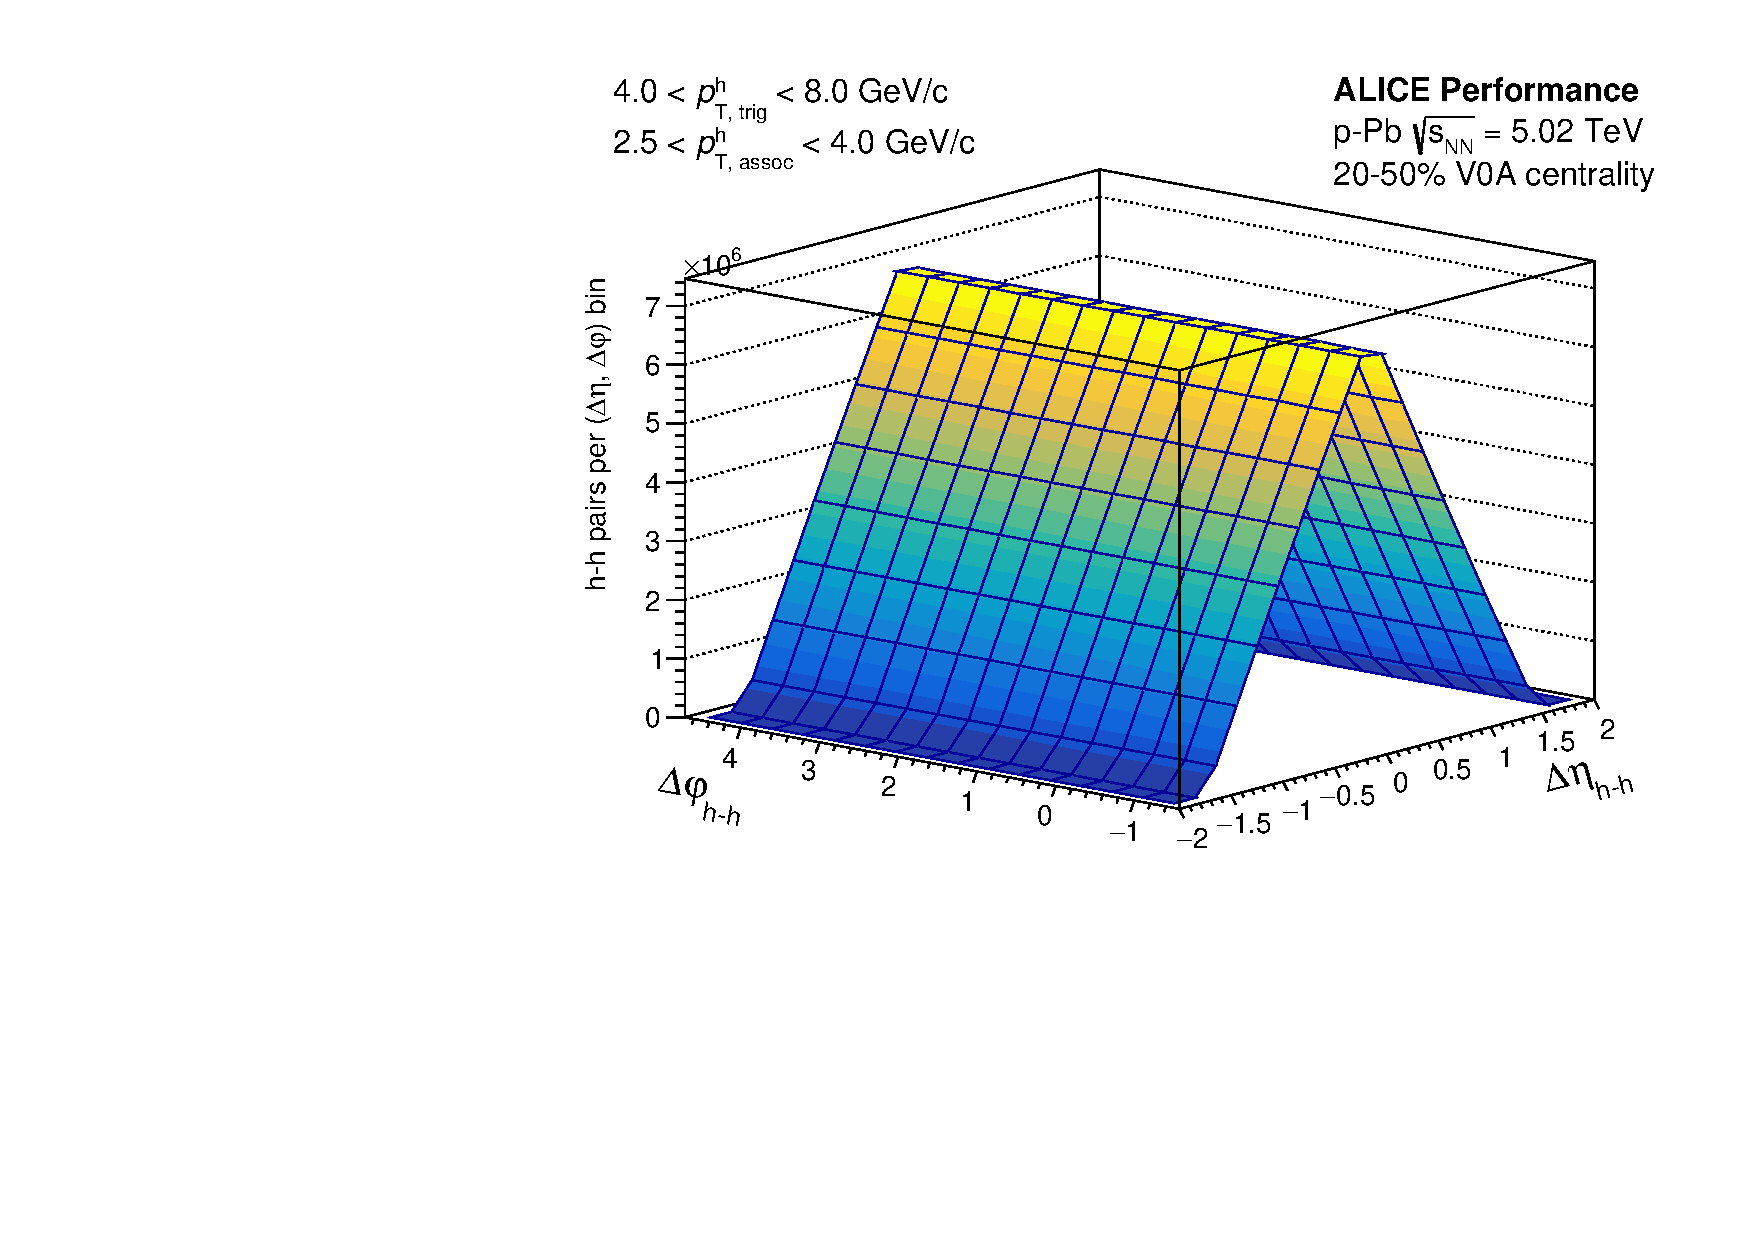
\includegraphics[width=\textwidth]{figures/analysis/h_h_2d_mixed_fancy_label_20_50_highpt.pdf}
	\end{minipage}
	\begin{minipage}{0.48\textwidth}
		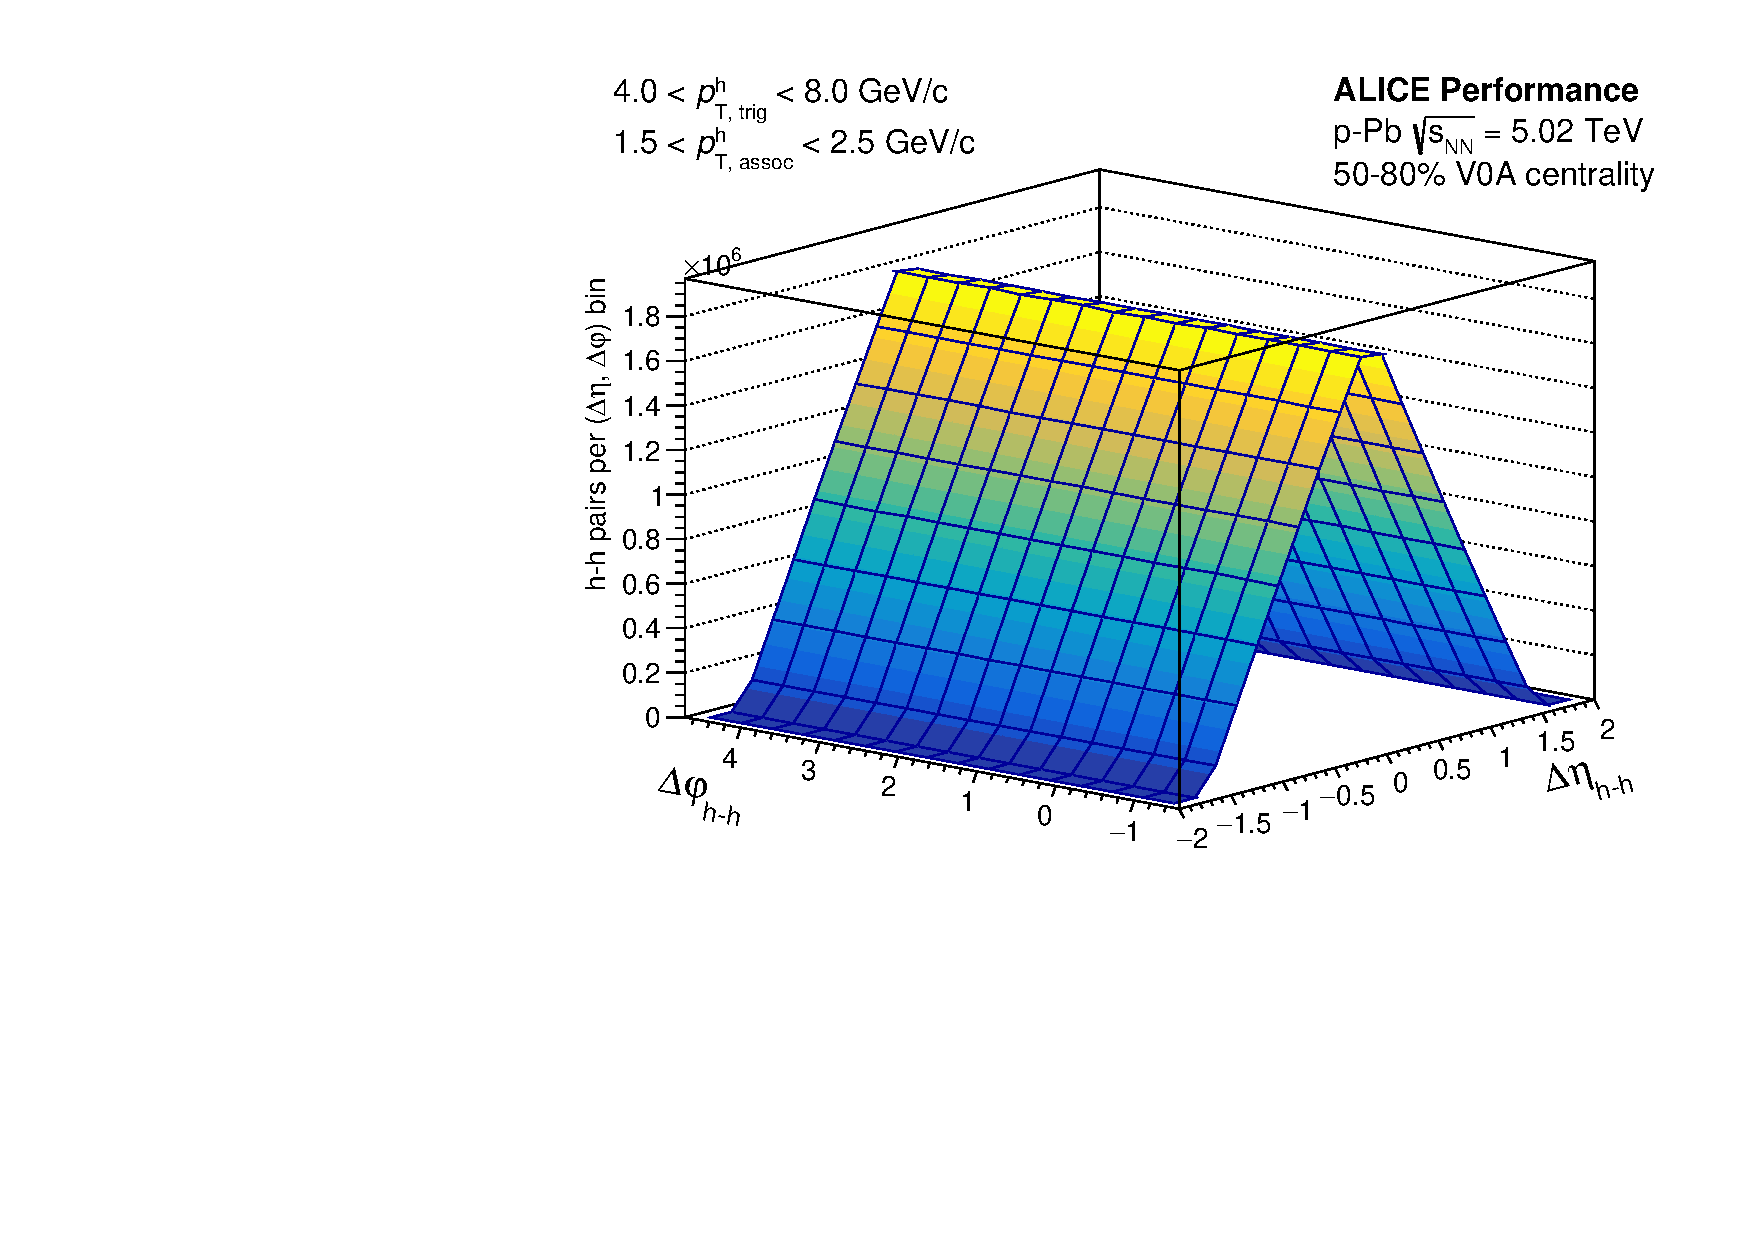
\includegraphics[width=\textwidth]{figures/analysis/h_h_2d_mixed_fancy_label_50_80_lowpt.pdf}
	\end{minipage}
	\begin{minipage}{0.48\textwidth}
		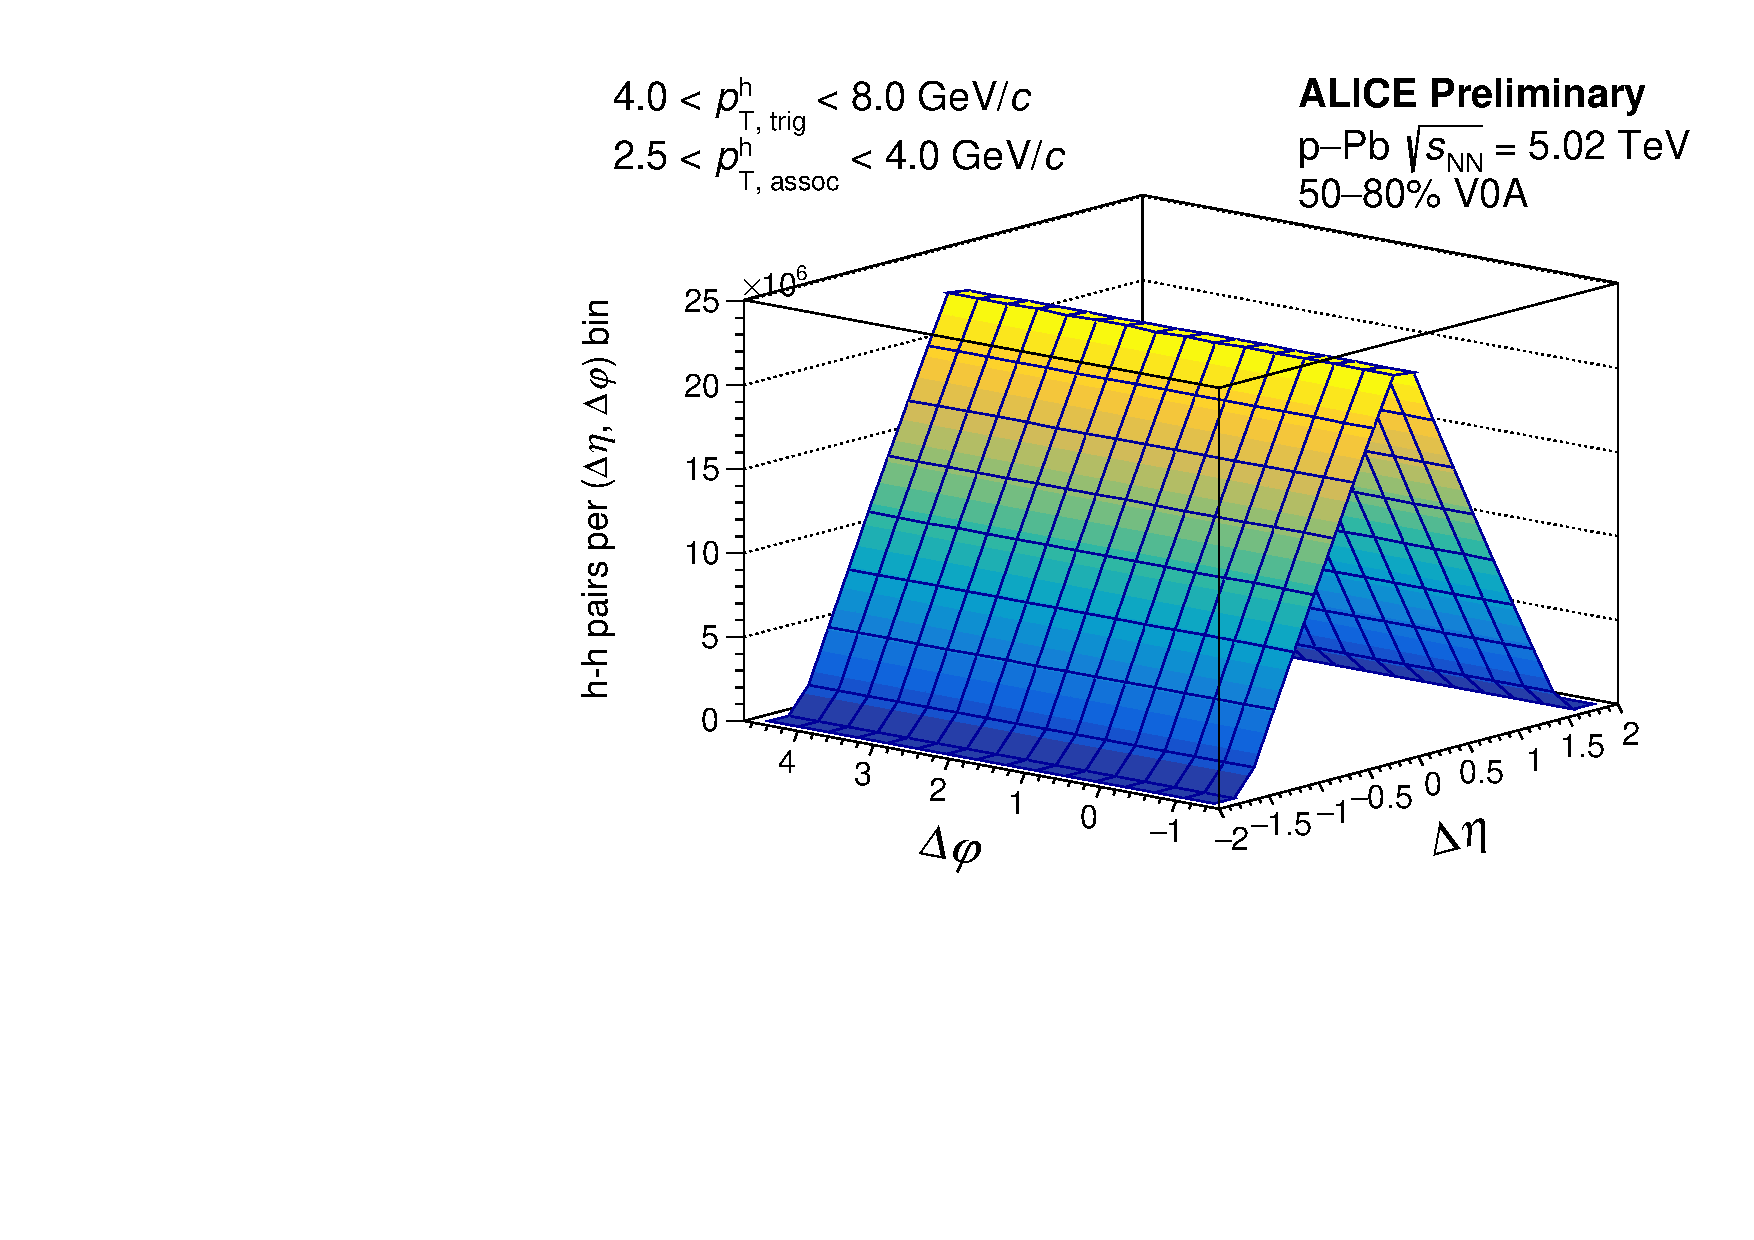
\includegraphics[width=\textwidth]{figures/analysis/h_h_2d_mixed_fancy_label_50_80_highpt.pdf}
	\end{minipage}
	\caption{2-D mixed-event h-h angular correlations for the 0-20\% (top), 20-50\% (middle), and 50-80\% (bottom) multiplicity bins for $1.5 < p_{\text{T}} < 2.5$ GeV/$c$ (left) and $2.5 < p_{\text{T}} < 4.0$ GeV/$c$ (right). The $Z_{\text{vtx.}}$ bins are merged together for these plots.}
	\label{fig:h_h_2d_mixed}
\end{figure}


This mixed-event correction is the final correction applied to the h-h distributions. However, the h-$\Lambda$ distributions require additional corrections that are not present in the dihadron case.

\clearpage

\subsection{Additional corrections for the h-$\Lambda$ distributions}
\label{sec:lambda_corrections}

While the corrected correlation function from Equation~\ref{eq:corr_detector} is generally true for two-particle correlations, there are a few additional corrections that must be applied to the h-$\Lambda$ distributions due to the $\Lambda$ reconstruction procedure and the presence of track merging effects. To formalize this, the corrected h-$\Lambda$ correlation function can be written as
%
\begin{align}
	\begin{split}
		C_{\text{corr.}}^{\text{h-}\Lambda}(\Delta\varphi, \Delta\eta) = \frac{r_{\text{signal}} \times r_{\text{branch}}}{\epsilon_{\text{pair}}(\Delta\varphi, \Delta\eta)}\biggl(&C_{\text{signal}}^{\text{h-p}\pi}(\Delta\varphi, \Delta\eta)\\
		&- r_{\text{comb.}} \times C_{\text{sideband}}^{\text{h-p}\pi}(\Delta\varphi, \Delta\eta)\biggr),
	\end{split}
	\label{eq:lambda_corr}
\end{align}
%
where $C_{\text{corr.}}^{\text{h-}\Lambda}$ is the final corrected h-$\Lambda$ distribution. Each term on the RHS of the equation will be described in detail in the following sections, and they are presented in the order in which they are applied to the distributions.

\subsubsection{Combinatorial background removal}
\label{sec:comb_bg_removal}

The term
%
\begin{equation}
C_{\text{signal}}^{\text{h-p}\pi}(\Delta\varphi, \Delta\eta) - r_{\text{comb.}} \times C_{\text{SB, norm.}}^{\text{h-p}\pi}(\Delta\varphi, \Delta\eta)
\end{equation}
%
describes the removal of the combinatorial backround resulting from the $\Lambda$ reconstruction procedure from Section~\ref{sec:lambda_reconstruction} using the \textbf{sideband subtraction} technique. The $C_{\text{signal}}^{\text{h-p}\pi}$ distribution corresponds to $\Lambda$ candidates where the invariant mass of the p$\pi$ pair falls within the range specified in Table~\ref{tab:lambda_selection}, and the self-normalized $C_{\text{SB, norm.}}^{\text{h-p}\pi}$ distribution corresponds to candidates where the mass of the p$\pi$ pair falls within the so-called ``sideband'' region. An invariant mass plot highlighting these different regions can be seen in Figure~\ref{fig:signal_sideband_regions}. Both of the $C_{\text{signal}}$ and $C_{\text{sideband}}$ distributions are corrected for acceptance and efficiency using the techniques described in the previous sections. The sideband region is chosen such that it is far enough away from the signal region to be free of any $\Lambda$ signal, but close enough to ensure that the background p$\pi$ pairs in the signal region are kinematically similar to the pairs in the sideband region as to not introduce any biases in the correlations. The underlying assumption of this technique is that the correlation shape of h-p$\pi$ pairs from the sideband region is the same as the shape from the background h-p$\pi$ pairs in the signal region. For this analysis, the nominal sideband region was chosen to be $1.135 < M_{p\pi} < 1.150$ \GeVmass, but the effects of varying this region are studied in detail in the next chapter. The $r_{\text{comb.}}$ is the integral of the combinatorial background in the $C_{\text{signal}}^{\text{h-p}\pi}$  distribution, obtained by 
%
\begin{equation}
	r_{Comb} \equiv \frac{B}{S+B} \int\int C_{\text{signal}}^{\text{h-p}\pi}(\Delta\varphi, \Delta\eta) d\Delta\varphi d\Delta\eta,
\end{equation}
%
where $S$ and $B$ are the signal and background obtained from the fits to the $\Lambda$ invariant mass distributions in Figure~\ref{fig:lambda_mass}. As the $S$/$B$ ratio is the same for the $\Lambda$ invariant mass distributions in events with a trigger hadron as it is for the h-$\Lambda$ distributions, the scale $B/(S+B)$ can be used to give only the background contribution from the integral $\int\int C_{\text{signal}}^{\text{h-p}\pi}(\Delta\varphi, \Delta\eta) d\Delta\varphi d\Delta\eta$. The self-normalized $C_{\text{SB, norm.}}^{\text{h-p}\pi}$ distribution is then scaled by $r_{\text{comb.}}$ and subtracted from $C_{\text{signal}}^{\text{h-p}\pi}$ to remove the combinatorial background.

\begin{figure}[ht]
	\centering
	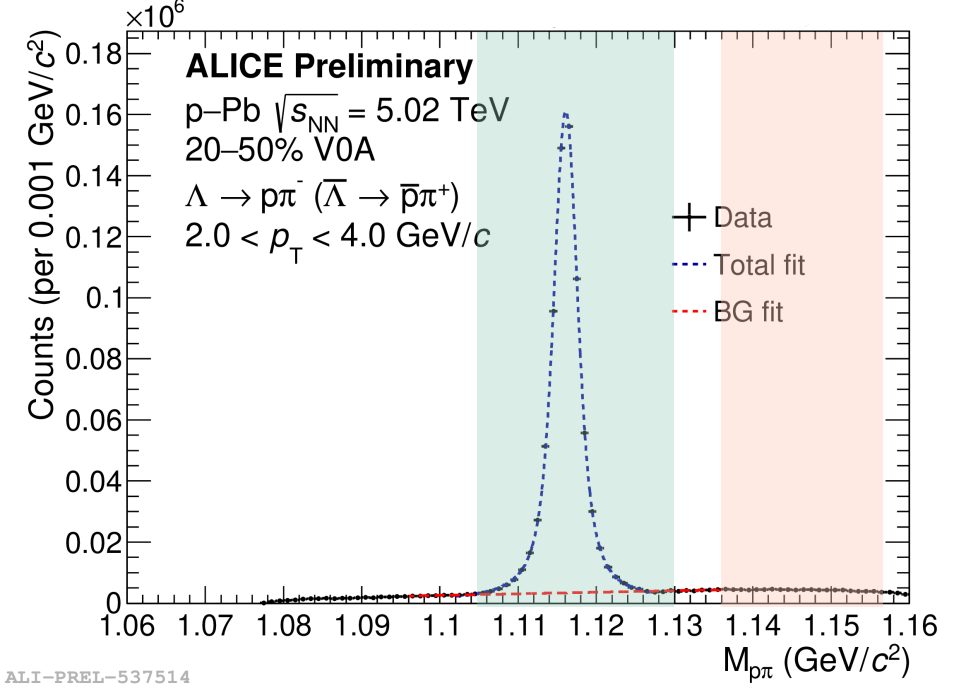
\includegraphics[width=0.8\textwidth]{figures/analysis/lambda_mass_regions.png}
	\caption{Invariant mass distribution of p$\pi$ pairs in the 20-50\% multiplicity class. The signal region is shown in light green, and the sideband region is shown in light pink. The correlation distribution in the sideband region is used to remove the combinatorial background from the signal region.}
	\label{fig:signal_sideband_regions}
\end{figure}

While the above procedure desribes the background removal in a more technical manner, it can be condensed into the following steps:
%
\begin{enumerate}
	\item Generate the correlation distribution using $\Lambda$ candidates in the signal invariant mass region
	\item Do the same thing for $\Lambda$ candidates in the sideband invariant mass region
	\item Scale the sideband distribution to match the background in the signal region
	\item Subtract the sideband distribution from the signal distribution
\end{enumerate}
%
Examples of the signal and sideband distributions $C_{\text{signal}}^{\text{h-p}\pi}$ and $C_{\text{SB}}^{\text{h-p}\pi}$ are shown for the 0-20\% multiplicity bin in Figure~\ref{fig:lambda_signal_sideband}.

\begin{figure}[ht]
	\centering
	\begin{minipage}{0.48\textwidth}
		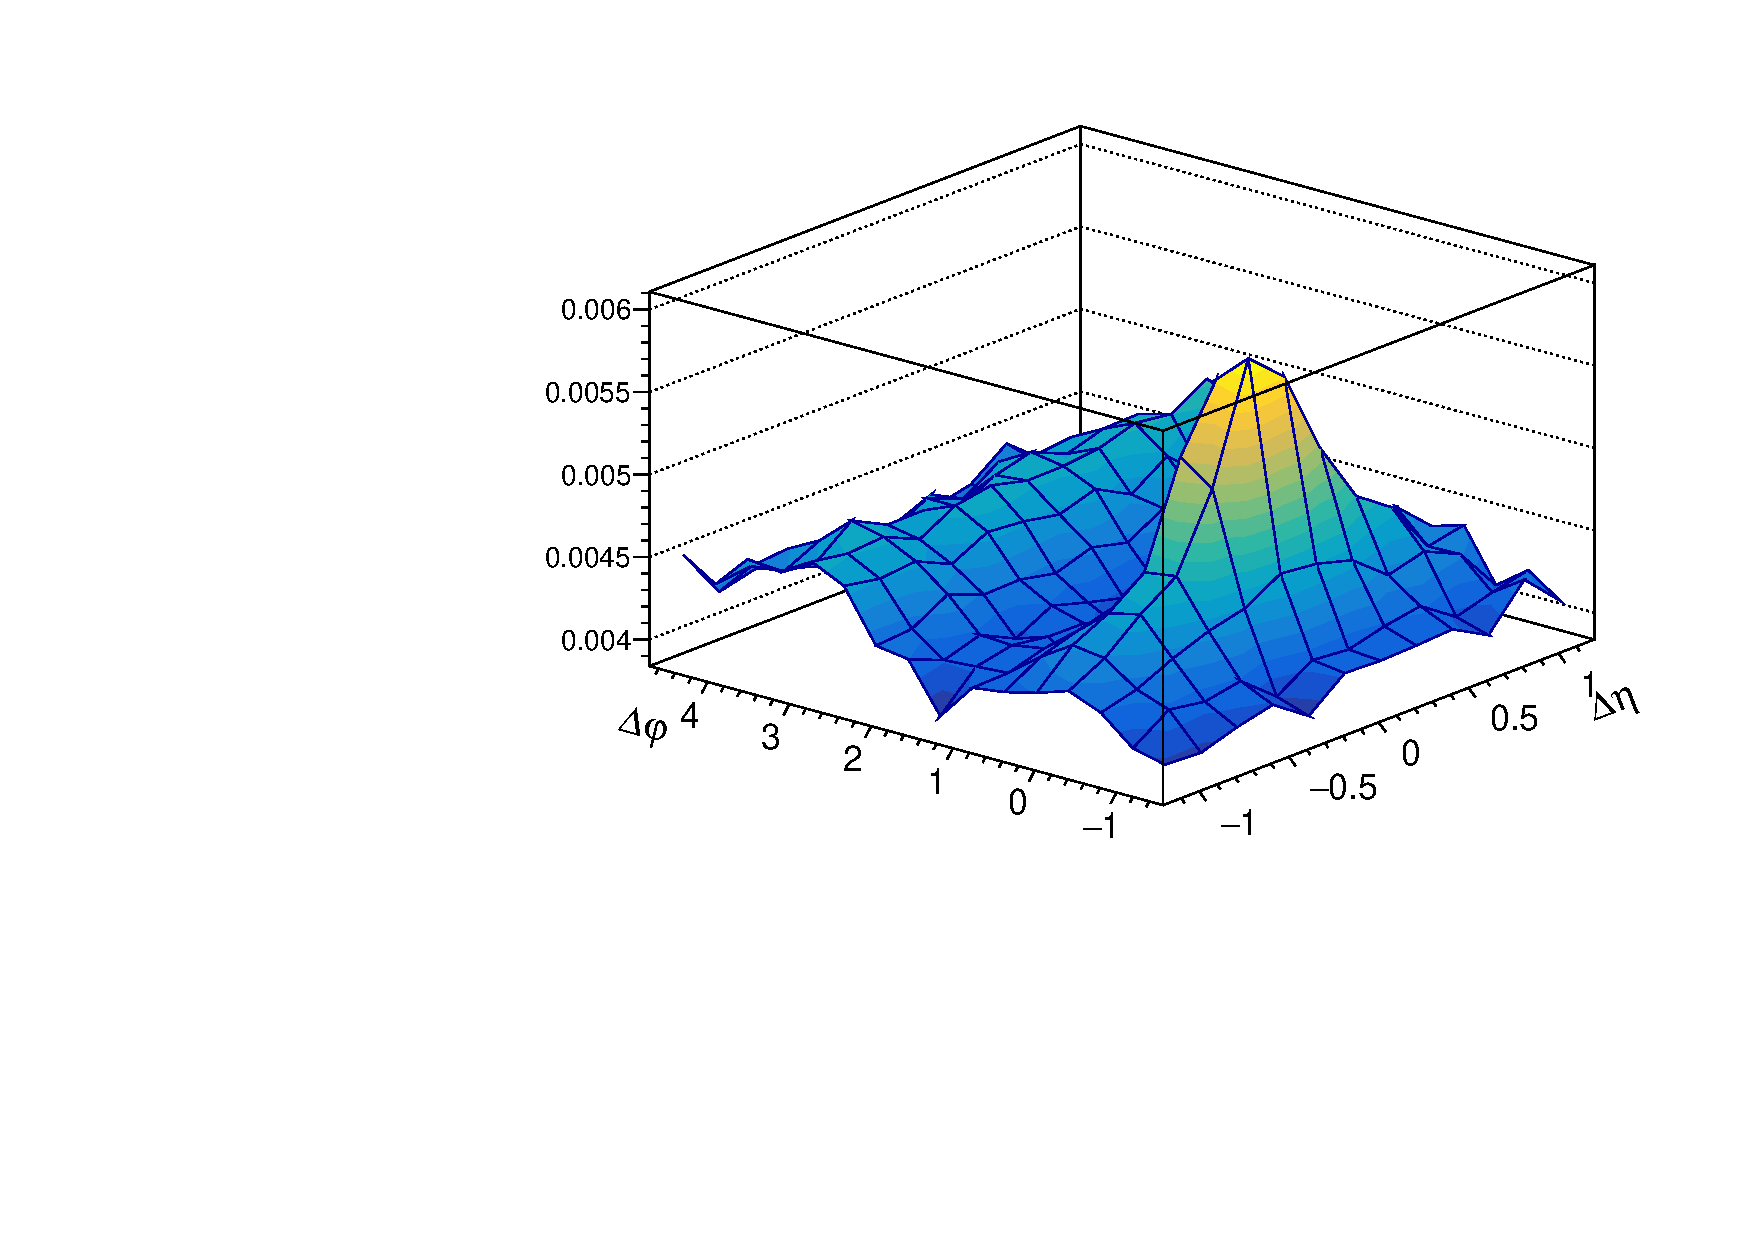
\includegraphics[width=\textwidth]{figures/analysis/h_lambda_sig_dist_lowpt.pdf}
	\end{minipage}
	\begin{minipage}{0.48\textwidth}
		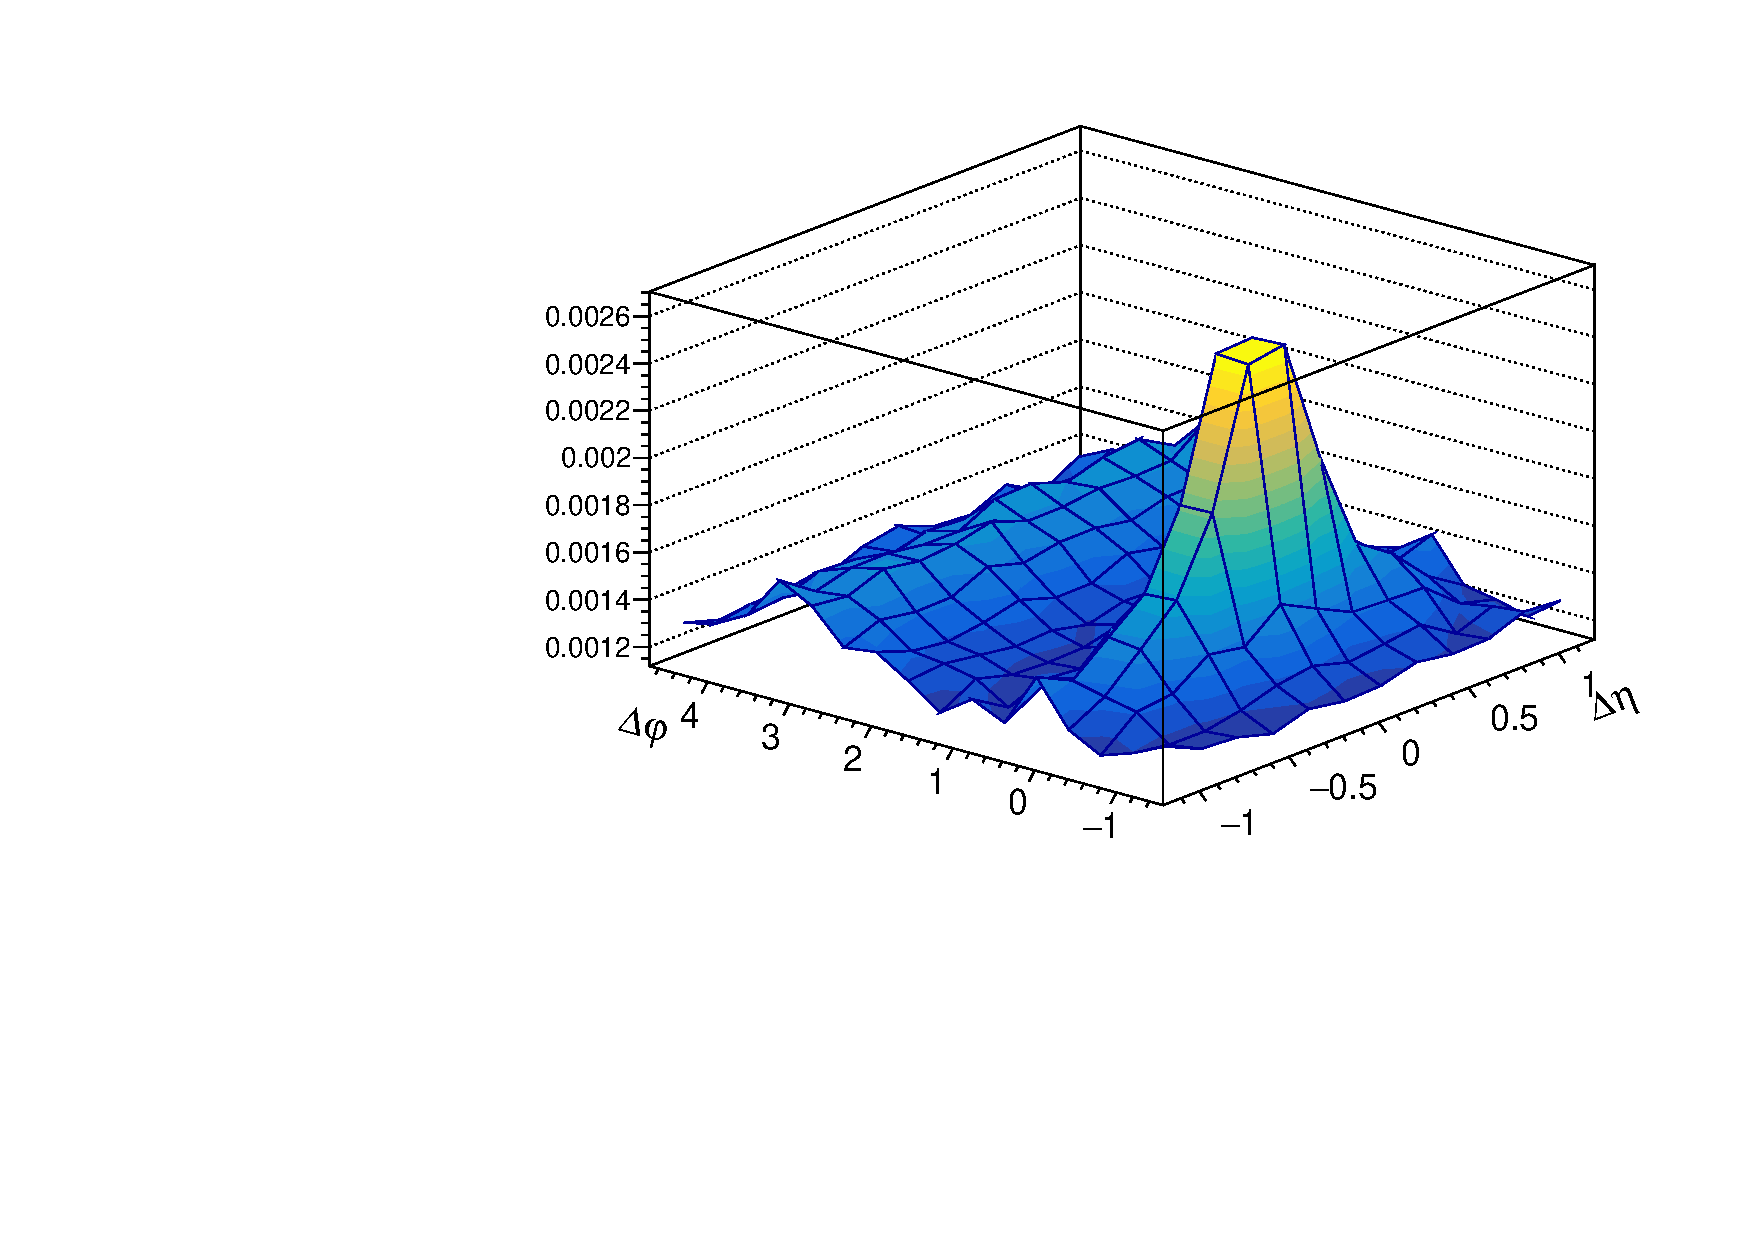
\includegraphics[width=\textwidth]{figures/analysis/h_lambda_sig_dist_highpt.pdf}
	\end{minipage}
	\begin{minipage}{0.48\textwidth}
		\includegraphics[width=\textwidth]{figures/analysis/h_lambda_rsb_dist_lowpt.pdf}
	\end{minipage}
	\begin{minipage}{0.48\textwidth}
		\includegraphics[width=\textwidth]{figures/analysis/h_lambda_rsb_dist_highpt.pdf}
	\end{minipage}
	\caption{The signal (top) and sideband (bottom) distributions $C_{\text{signal}}^{\text{h-p}\pi}$ and $C_{\text{SB}}^{\text{h-p}\pi}$ for the lower (left) and higher (right) associated \pt bins. All plots were generated in the 0-20\% multiplicity class.}
	\label{fig:lambda_signal_sideband}
\end{figure}

\subsubsection{Signal scaling}

As the $\Lambda$ candidate invariant mass signal region is finite, the fraction of the $\Lambda$ signal that is missed in the tails of the invariant mass distribution must be corrected for. This is handled by the $r_{\text{signal}}$ term in Equation~\ref{eq:lambda_corr}, which is calculated by 
%
\begin{equation}
	\label{eq:signal_scaling}
	r_{\text{signal}} \equiv (\frac{\text{Integral of residual in signal region}}{\text{Integral of residual between 1.098 and 1.134}})^{-1}
\end{equation}
%
where ``residual'' refers to the invariant mass distributions from Figure~\ref{fig:lambda_mass} after subtracting the straight-line background fit. 1.098 and 1.134 are the points in which there is effectively zero signal, verified in Monte Carlo. Due to the width of the signal region, $r_{\text{signal}}$ is usually near unity. However, to study the effects of narrowing the signal region, this term must be included in the analysis.

\subsubsection{Branching ratio correction}

The most simple correction from Equation~\ref{eq:lambda_corr} comes from the branching ratio term, namely 
%
\begin{equation}
	r_{\text{branch}} \equiv \frac{1}{BR(\Lambda \rightarrow p\pi)} = \frac{1}{0.639}.
\end{equation}
%
As not all $\Lambda$s decay into p$\pi$ pairs, this term corrects for the fraction of $\Lambda$s that decided to decay into something else. In many analyses, this term is not required, as it is already included in the efficiency computation $\epsilon_{\text{assoc.}}$. As the $\Lambda$ reconstruction efficiency from this analysis is calculated using only $\Lambda$s that decay into p$\pi$ pairs, this term must be included separately. 

\subsubsection{Pair efficiency correction}
\label{sec:pair_eff_corr}

The $\epsilon_{\text{pair}}$ term in Equation~\ref{eq:lambda_corr} is the h-$\Lambda$ ``pair'' efficiency, which is used to correct for track merging effects. Many correlation studies are susceptible to track merging inefficiencies~\cite{TwoTrack1, TwoTrack2}, whereby either the trigger or associated particle gets merged over by the other during the track reconstruction. This results in a dip at small angles in the angular correlation distribution when compared to a similar distribution with no instances of track merging. As this effect cannot be seen directly in data due to the missing reconstructed tracks, it is investigated using the Monte Carlo sample, where the reconstructed tracks are compared to the MC-generated particles they were reconstructed from. While this effect is usually negligible and only relevant at extremely small angles ($\Delta\varphi < 0.01, \Delta\eta < 0.1$), in this analysis this effect is more severe and occurs at larger angles ($\Delta\varphi < 1, \Delta\eta < 0.6$), shown in Figure \ref{fig:trackmerge_diagram_lambda}. 

\begin{figure}[ht]
	\centering
	\begin{minipage}{0.48\textwidth}
		\includegraphics[width=\textwidth]{figures/analysis/trackmerge_lambda_dphi_small_deta.pdf}
	\end{minipage}
	\begin{minipage}{0.48\textwidth}
		\includegraphics[width=\textwidth]{figures/analysis/trackmerge_lambda_dphi_large_deta.pdf}
	\end{minipage}
	\caption{Demonstration of the track merging effect for h-$\Lambda$ pairs, whereby we see a dip in the reconstructed distribution at small $\Delta\varphi$ and $\Delta\eta$ when compared to the MC ground truth (left). This dip is not present at large $\Delta\eta$ (right), but we also lose nearly the entirety of our near-side peak.}
	\label{fig:trackmerge_diagram_lambda}
\end{figure}

The severity of this effect for the h-$\Lambda$ distributions is likely due to two factors:
%
\begin{itemize}
\item The $\Lambda$ decay length is large ($c\tau \approx 10$ cm), meaning the daughter particles will have less hits in the detector than the trigger particle (which is produced at the primary vertex). As Kalman filtering~\cite{Kalman} (track reconstruction) favors the track with more hits, the $\Lambda$ daughter track is ``merged'' over by the trigger track.
\item The $\Lambda$ decay is asymmetric ($m_{p}/m_{\pi} \approx 7$), so the $\Lambda$ and daughter proton end up with similar momenta (and thus $\varphi$ and $\eta$). This means that whenever a proton from a $\Lambda$ decay is ``merged'' over by a trigger track, a h-$\Lambda$ pair with small $\Delta\varphi, \Delta\eta$ is lost.
\end{itemize}
%
To see how the decay length can affect the track merging, the (reconstructed)/(MC ground-truth) $C(\Delta\varphi, \Delta\eta)$ distribution ratio for h-pion pairs in our MonteCarlo sample where the pion is \textbf{secondary}--meaning it came from a weak decay with decay length $>$ 2cm--is measured. Pions are chosen for this demonstration as they are more abundantly produced than protons, and charged track reconstruction is particle species agnostic. Any ``dips'' from unity present in this ratio are indicative of pairs being lost during reconstruction. This is then compared to the same ratio for $h-$pion pairs where the pion is \textbf{primary}, and the results are shown in Figure~\ref{fig:trackmerge_hpion}. All reconstructed triggers and pions pass the trigger hadron and $\Lambda$ daughter cuts from Tables \ref{tab:trigger_track_cuts} and \ref{tab:lambda_daughter_track_cuts}, respectively. Furthermore, all distributions have been fully corrected for single-particle efficiencies and detector acceptance using the procedures from Sections~\ref{sec:single_particle_corr} and~\ref{sec:acceptance_corr}, respectively. A large suppression at small $(\Delta\varphi, \Delta\eta)$ is observed for the h-secondary pion case, but the h-primary pion case exhibits no such supression. As such, it stands to reason that this suppression is at least in part due to the decay length of the $\Lambda$, as all particles that come from $\Lambda$s are secondaries (by a long shot).

\begin{figure}[ht]
	\centering
	\begin{minipage}{0.48\textwidth}
		\includegraphics[width=\textwidth]{figures/analysis/h_pion_2d_secondary.png}
	\end{minipage}
	\begin{minipage}{0.48\textwidth}
		\includegraphics[width=\textwidth]{figures/analysis/h_pion_2d_primary.png}
	\end{minipage}
	\caption{The  reconstructed/ground truth ratios of the 2D $C(\Delta\varphi, \Delta\eta)$ distributions for h-(secondary pions) (left) and h-(primary pions) (right). The suppression at smaller $\Delta\varphi, \Delta\eta$ is clearly seen in the secondary case, but is not observable in the primary case, indicating a decay-length dependence.}
	\label{fig:trackmerge_hpion}
\end{figure}

The $p_\text{T}$ dependence of this effect can also be studied by measuring the reconstructed and ground truth $h-$(secondary pion) $\Delta\varphi$ distributions at low ($1.0 < p_{\text{T}} < 2.0$ \GeVc) and high ($2.0 < p_{\text{T}} < 4.0$ \GeVc) associated momentum. The result is shown in Figure \ref{fig:trackmerge_pt_dependence}. Note that the distributions were projected onto $\Delta\varphi$ with $|\Delta\eta| < 1.2$. A suppression relative to MC ground-truth is observed in the near-side of the reconstructed distribution in the higher $p_\text{T}$ range, which is not seen in the low $p_\text{T}$ bin. This is also consistent with the decay length dependence shown in the previous figures, as decay length is roughly proportional to $p_\text{T}$.

\begin{figure}[ht]
	\centering
	\begin{minipage}{0.48\textwidth}
		\includegraphics[width=\textwidth]{figures/analysis/h_pion_dphi_secondary_0_2.pdf}
	\end{minipage}
	\begin{minipage}{0.48\textwidth}
		\includegraphics[width=\textwidth]{figures/analysis/h_pion_dphi_secondary_2_4.pdf}
	\end{minipage}
	\caption{The reconstructed and ground truth $\Delta\varphi$  distributions in the $-1.2 < \Delta\eta < 1.2$ region for h-(secondary pions) with $0.15 < p_{\text{T}} < 2$ (left) and $2 < p_{\text{T}} < 4$ (right). The suppression at smaller $\Delta\eta, \Delta\varphi$ is clearly seen in the higher momentum bin, but not present in the lower one.}
	\label{fig:trackmerge_pt_dependence}
\end{figure}

The $p_{T}$ dependence of this inefficiency demonstrates why this effect is so severe in the h-$\Lambda$ case: due to the asymmetry of the $\Lambda$ decay ($m_{\text{p}}/m_{\pi} \approx 7$), the daughter proton receives most of the momentum. Therefore when investigating h-$\Lambda$ correlations within a given associated \pt range, any inefficiencies present in the corresponding h-(daughter proton) distribution with the same associated momentum would also be present in our final h-$\Lambda$ distribution within a similar $\Delta\varphi, \Delta\eta$ range. As demonstrated in Figure \ref{fig:trackmerge_pt_dependence}, secondary charged particles with $2 < p_{T} < 4$ GeV/c see a large inefficiency, and therefore we would expect a similar inefficiency to be present in our h-$\Lambda$ distribution (which was shown in Figure \ref{fig:trackmerge_diagram_lambda}). In similar analyses using the $\text{K}^{0}_{\text{S}}$ in leiu if the $\Lambda$~\cite{Lambda1}, such an effect is not as present, both because the decay length is much shorter (2 cm vs 10 cm), and the $\text{K}^{0}_{\text{S}}$ decay is symmetric, meaning the daughter pions will have momenta that are no longer similar to the mother kaon.

The folling techniques have been investigated to correct for this effect:
%
\begin{itemize}
	\item Applying a $\Delta\varphi^{*}$ correction, which accounts for the helical nature of the tracks in the detector, as described in~\cite{DphiStar}: While $\Delta\varphi$ and $\Delta\varphi^{*}$ are different, they are correlated enough that in order to remove this effect, a $|\Delta\varphi^{*}| < 0.7$ cut is required, which removes a significant amount of the near-side yield in the corresponding $\Delta\varphi$ distribution.
	\item Applying a cut on the minimum distance between the fully reconstructed helices of the trigger and $\Lambda$ daughter proton (varied between 0.1 cm and 10 cm): Again, this cut removes roughly the same amount of near-side yield as the $\Delta\varphi^{*}$ cut, as this minimum distance is also highly correlated with $\Delta\varphi$.
	\item Using the resonance technique for $\Lambda$ reconstruction (more details in Section \ref{sec:resonance_technique}): This moderately reduces the severity of this effect, but the statistical fluctuations introduced by the smaller S/B ratio make it difficult to gauge how effective this correction is.
	\item Only correlating h-$\Lambda$ pairs where the charge of the $\Lambda$ daughter proton (or antiproton) is opposite to the trigger, as oppositely charged tracks bend in opposite directions in the detector magnet: This reduces the effect by a considerable amount, but reduces our overall correlation statistics by a factor of 2.
	\item Selecting ``lower quality'' trigger tracks by loosening the cuts from Table~\ref{tab:trigger_track_cuts} so they are less likely to be merged over the low-quality daughter tracks: This reduces the effect, but introduces a large amount of secondary contamination. Furthermore, we would like this analysis to be directly compared with other analyses, and therefore want to maintain the same cuts on the trigger hadron.
	\item Selecting ``higher quality'' $\Lambda$ daughter tracks by tightening the cuts from Table~\ref{tab:lambda_daughter_track_cuts} (and adding additional selection criteria): This again reduces the effect but heavily cuts into the $\Lambda$ signal
\end{itemize}
%
As each of these techniques reduces the statistics of the h-$\Lambda$ correlation distribution beyond the realm of acceptability, the two-track inefficiencies are instead corrected for using a MC-generated template method, similar to the one used in~\cite{TwoTrack2}. For this method, the pair efficiency is given by
%
\begin{equation}
    \epsilon_{pair}(\Delta\varphi, \Delta\eta) \equiv \frac{C_{\text{reco}}^{\text{tag}}(\Delta\varphi, \Delta\eta)}{C_{\text{gen}}(\Delta\varphi, \Delta\eta)},
\label{eq:paircorr}
\end{equation}
%
where $C_{\text{reco}}^{\text{tag}}$ is the efficiency-corrected correlation distribution calculated in MC using reconstructed trigger hadrons and $\Lambda$ candidates with the same selection criteria as described in Section~\ref{sec:track_selection}, with the additional requirement that the $\Lambda$ candidate has a corresponding generated $\Lambda$ which is used for all calculations involving kinematic quantities. This removes the need to perform any of the additional corrections from the previous sections (e.g. background subtraction, signal scaling) as the invariant mass of generated lambdas is exact. $C_{gen}$ is the correlation distribution calculated in MC using only generated trigger hadrons and $\Lambda$ candidates. The template $\epsilon_{pair}(\Delta\varphi, \Delta\eta)$ is applied for each associated \pt bin in this analysis, but it is independent of multiplicity and event generator. The templates for each associated \pt bin are shown in Figure~\ref{fig:pair_efficiency_template}. This correction is applied to the h-$\Lambda$ distributions after side-band subtraction, signal scaling, and the branching ratio correction.

\begin{figure}[ht]
	\centering
	\begin{minipage}{0.48\textwidth}
		\includegraphics[width=\textwidth]{figures/analysis/twotrack_template_lowpt.pdf}
	\end{minipage}
	\begin{minipage}{0.48\textwidth}
		\includegraphics[width=\textwidth]{figures/analysis/twotrack_template_highpt.pdf}
	\end{minipage}
	\caption{The $\epsilon_{\text{pair}}(\Delta\varphi, \Delta\eta)$ templates for the track merging correction in the lower ($1.5 <$ \pt $< 2.5$ \GeVc, left)  and higher ($2.5 <$ \pt $< 4.0$ \GeVc, right) associated momentum bins. While it may be difficult to observe, the lower \pt bin has a minimum dip of around 0.84, whereas the higher \pt bin has a minimum dip of around 0.81, reflecting the \pt dependence discussed in this section.}
	\label{fig:pair_efficiency_template}
\end{figure}

After these corrections, both the h-$\Lambda$ and h-h 2D distributions are finalized and ready for projection onto $\Delta\varphi$ to extract the yields and widths of interest from the previous chapter. These fully corrected distributions can be seen in Figures~\ref{fig:h_lambda_2d_final} (h-\lmb) and~\ref{fig:h_h_2d_final} (h-h). However, there are still a number of systematic uncertainties to investigate and cross-checks required to ensure the validity of the final results.

\begin{figure}[ht]
	\centering
	\begin{minipage}{0.48\textwidth}
		\includegraphics[width=\textwidth]{figures/analysis/h_lambda_2d_mixcor_fancy_label_0_20_lowpt.pdf}
	\end{minipage}
	\begin{minipage}{0.48\textwidth}
		\includegraphics[width=\textwidth]{figures/analysis/h_lambda_2d_mixcor_fancy_label_0_20_highpt.pdf}
	\end{minipage}
	\begin{minipage}{0.48\textwidth}
		\includegraphics[width=\textwidth]{figures/analysis/h_lambda_2d_mixcor_fancy_label_20_50_lowpt.pdf}
	\end{minipage}
	\begin{minipage}{0.48\textwidth}
		\includegraphics[width=\textwidth]{figures/analysis/h_lambda_2d_mixcor_fancy_label_20_50_highpt.pdf}
	\end{minipage}
	\begin{minipage}{0.48\textwidth}
		\includegraphics[width=\textwidth]{figures/analysis/h_lambda_2d_mixcor_fancy_label_50_80_lowpt.pdf}
	\end{minipage}
	\begin{minipage}{0.48\textwidth}
		\includegraphics[width=\textwidth]{figures/analysis/h_lambda_2d_mixcor_fancy_label_50_80_highpt.pdf}
	\end{minipage}
	\caption{2-D fully-corrected h-$\Lambda$ angular correlations for the 0-20\% (top), 20-50\% (middle), and 50-80\% (bottom) multiplicity bins for $1.5 < p_{\text{T}} < 2.5$ GeV/$c$ (left) and $2.5 < p_{\text{T}} < 4.0$ GeV/$c$ (right).}
	\label{fig:h_lambda_2d_final}
\end{figure}
\begin{figure}[ht]
	\centering
	\begin{minipage}{0.48\textwidth}
		\includegraphics[width=\textwidth]{figures/analysis/h_h_2d_mixcor_fancy_label_0_20_lowpt.pdf}
	\end{minipage}
	\begin{minipage}{0.48\textwidth}
		\includegraphics[width=\textwidth]{figures/analysis/h_h_2d_mixcor_fancy_label_0_20_highpt.pdf}
	\end{minipage}
	\begin{minipage}{0.48\textwidth}
		\includegraphics[width=\textwidth]{figures/analysis/h_h_2d_mixcor_fancy_label_20_50_lowpt.pdf}
	\end{minipage}
	\begin{minipage}{0.48\textwidth}
		\includegraphics[width=\textwidth]{figures/analysis/h_h_2d_mixcor_fancy_label_20_50_highpt.pdf}
	\end{minipage}
	\begin{minipage}{0.48\textwidth}
		\includegraphics[width=\textwidth]{figures/analysis/h_h_2d_mixcor_fancy_label_50_80_lowpt.pdf}
	\end{minipage}
	\begin{minipage}{0.48\textwidth}
		\includegraphics[width=\textwidth]{figures/analysis/h_h_2d_mixcor_fancy_label_50_80_highpt.pdf}
	\end{minipage}
	\caption{2-D fully-corrected h-h angular correlations for the 0-20\% (top), 20-50\% (middle), and 50-80\% (bottom) multiplicity bins for $1.5 < p_{\text{T}} < 2.5$ GeV/$c$ (left) and $2.5 < p_{\text{T}} < 4.0$ GeV/$c$ (right).}
	\label{fig:h_h_2d_final}
\end{figure}

\clearpage